\typeout{NT FILE STATE-ART.tex}%
\chapter{Background and Related Work}%
\label{ch:state-art}
%
\begin{quote}
\begin{flushright}
``\emph{We stand on the shoulders of giants.}'' \\
\textbf{-- Isaac Newton}, mathematician, physicist, astronomer
\end{flushright}
\end{quote}

This chapter establishes the technical context for the thesis. We begin with mixed-criticality systems (\glspl{mcs}): why they matter, where they appear, and the challenges they pose for timing predictability, isolation, and assurance under practical \gls{swap-c} constraints. We then outline the current approach to manage this complexity, highlighting the trade-offs they introduce.
%
Next, we survey \glspl{uav}'s reference hardware and software
stacks, covering both open-source and commercial solutions, with emphasis on
properties relevant to mixed-critical deployments (e.g., platform support,
determinism, and isolation).
%
Finally, we review related work, organizing recent research along the axes most
pertinent to this thesis (flight stacks, onboard platforms, and
virtualization). This positions the contribution that follows and clarifies the
specific gaps the proposed design addresses.

% \section{Mixed criticality systems}%
% \label{sec:mixed-crit-syst}
% Embedded systems have stringent requirements both on timing and criticality of
% the tasks it performs. The former concerns the task's timing deadlines
% requirement (firm, soft, hard), whereas the latter is a
% designation of the level of assurance against failure needed for a system
% component~\cite{burns2022mixed}. Typical names for the criticality levels are
% \glspl{asil}, \glspl{dal}, and \glspl{sil}~\cite{burns2022mixed}.

% This is the case for \gls{uav}'s applications with real-time constraints but
% with mixed
% criticality levels, i.e., the risk of failure is more severe in some case than others.
% For example, flight control (safety-critical) and video streaming (non-critical)
% coexist. A compromise in video software could cascade to flight systems, causing
% catastrophic failure—yet strict hardware separation increases weight and reduces
% flight time.

% This exemplifies a \gls{mcs}, i.e., a system comprised of computer hardware and
% software that executes several tasks/applications of distinct criticality (safety) levels.
% However, the integration of mixed-criticality components onto a common hardware
% platform is not an easy task: the designer needs to meet the stringent
% \gls{swap-c} metrics and safety requirements
% provided by safety-critical standards, such as those for automotive~\cite{iso26262}, avionics~\cite{rtca1992software},
% and railway~\cite{cenelec201250128} industries.
% While \gls{mcs} challenges are well-studied in automotive/avionics, UAVs face unique
% constraints: extreme SWaP-C limitations and the need for fail-operational safety
% in uncontrolled environments. Current solutions either compromise isolation
% (single-board) or add weight/energy overhead (multi-board).

% As a result of this integration
% complexity increases, requiring higher computational power, and thus, these
% hardware platforms are migrating from single cores to multi-cores and in the
% future many-core architectures~\cite{burns2022mixed}. This leads to the
% fundamental question of how to reconcile the
% conflicting requirements of \emph{partitioning} for (safety) assurance and \emph{sharing} for
% efficient resource usage. Consequently, problems arise in the modelling, design,
% implementation, and verification of the required hardware and
% software~\cite{burns2022mixed}.

% Two major areas of research stem from this dichotomy: a more theorethical one,
% largely focused on using criticality-specific \glspl{wcet} to schedule systems
% at each criticality level, but at the expenses of high processor utilization; a
% more practical one, focused on the safe partitioning of a system with the
% sharing of computational and communication resources, but with increased
% complexity.
% Unfortunately, the combination of both areas is not easy: flexible scheduling
% requires, at least, dynamic partitioning, whereas certified systems require
% complete separation or, at least, static partitioning. This mismatch needs to be
% addressed in future work~\cite{burns2022mixed}.

% Another important topic in the \gls{mcs} field is the the incorporation of other
% shared resources, e.g.~communication, particulary on multi-core or many-core
% platforms: can a shared bus provide the required separation, or is a
% Network-on-Chip protocol required? These issues are only now beginning to be
% addressed~\cite{burns2022mixed}.

\section{Mixed Criticality Systems}%
\label{sec:mixed-crit-syst}
Embedded platforms increasingly host many functions on the same hardware to
reduce size, weight, power, and cost
(\gls{swap-c})~\cite{burns2022mixed}. However, not all functions are equally
critical. In safety-regulated domains, strong guarantees are required to ensure
that consolidation does not compromise
safety~\cite{burns2022mixed,davis_mixed_2018}.
%
Standards such as ISO~26262~\cite{iso26262} and
DO-178C~\cite{sc_167_software_1992} formalize these assurances, particularly in
automotive and avionics. On one hand, consolidation pressures favor efficient
resource sharing to minimize \gls{swap-c}; on the other, domain isolation is
needed to ensure well-behaved applications.
The fundamental question in
\glspl{mcs} is how to reconcile these conflicting goals, i.e., providing strong
separation for assurance while enabling sharing for efficiency~\cite{burns2022mixed}. Addressing this
requires system design that integrates software and hardware on a single
platform, together with modeling, verification, and, where applicable,
certification~\cite{davis_mixed_2018,youn_software_2015}.

A \gls{mcs} is, simply, a system that integrates software components of two or
more criticality levels into the same platform~\cite{davis_mixed_2018}. Consider a \gls{uav} executing a
video-surveillance mission (Fig.~\ref{fig:mcs-example}). Tasks are color-coded
by criticality according to
the DO-178C standard~\cite{sc_167_software_1992,youn_software_2015}. The navigation and stability
are life-critical functions, i.e., flight-control loops must meet their deadlines under all
conditions, or catastrophic failure may occur. Accordingly, sensor acquisition
and communication handling, processing, and actuation must complete within
predefined time bounds. Here, \emph{criticality} denotes the assurance level
required to bound the probability of such failures~\cite{sc_167_software_1992,youn_software_2015}.

By contrast, obstacle avoidance and video capture are mission-critical. They
have soft real-time requirements, but their consequences differ: failing to
detect an obstacle may endanger the aircraft, whereas dropping camera frames is
generally acceptable. Lastly, auxiliary tasks such as logging and telemetry are
non-critical, as missing soft deadlines does not cause safety harm.

One consequence of applying the DO-178C safety standard at a system level is that all \gls{uav}
functions would need to be developed to the life-critical level of navigation
and stability~\cite{youn_software_2015,davis_mixed_2018}. In our case, that
would make “missing a camera frame” as unlikely -- and as costly to assure -- as
“missing an actuator output,” resulting in substantial over-engineering of
mission- and non-critical subsystems. The alternative is to demonstrate
\emph{temporal and spatial isolation}, i.e., that lower-assurance functions can
neither delay nor corrupt higher-assurance functions, even under
faults~\cite{cinque2022virtualizing,davis_mixed_2018}.

\begin{figure}[!hbt]
  \centering
  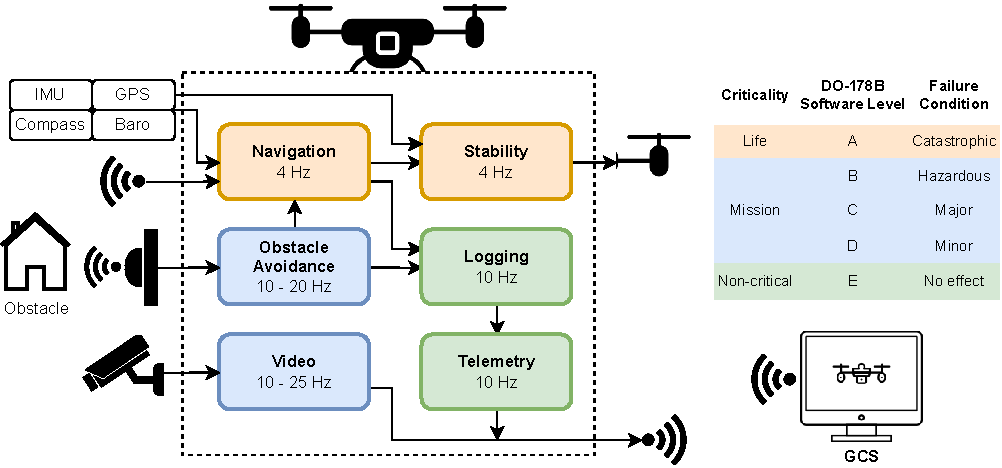
\includegraphics[width=1.0\textwidth]{./img/pdf/mcs-example}
  \caption[Mixed-criticality system example: UAV application]{Mixed-criticality system example: UAV application (adapted from~\cite{yip_relaxing_2014}).}%
  \label{fig:mcs-example}
\end{figure}

While \gls{mcs} principles apply broadly, \glspl{uav} face domain-specific
hurdles. They must meet extreme \gls{swap-c} limits: (1) every gram of weight
counts, especially in lower weight classes~\cite{alladi2022UAVBlockain}, affecting the \gls{uav}'s autonomy
and flight dynamics; (2) they operate in uncontrolled,
rapidly changing environments~\cite{faical_adaptive_2017}; (3) and must maintain critical functions during faults, since not every error can be
anticipated~\cite{mohsan2022towards}.
The
shift to mainstream multicore architectures further complicates resource
sharing~\cite{burns2022mixed}. Current approaches reveal a core trade-off: on
one hand, multi-board designs provide strong isolation but poor \gls{swap-c}
metrics; on the other, single-board designs improve \gls{swap-c} but weaken isolation.

Two major research branches stem from this dichotomy. A more \emph{theoretical}
line studies scheduling with criticality-dependent \glspl{wcet} to schedule
systems at each criticality level, but at the cost of higher processor utilization~\cite{lee_estimating_2023}. A more \emph{practical}
line focuses on safe partitioning with shared computational and communication
resources, at the cost of increased design complexity~\cite{cinque2022virtualizing}. Combining the two is
hard as flexible scheduling typically requires at least dynamic partitioning,
whereas certified systems favor complete separation or static
partitioning~\cite{burns2022mixed}. This gap is acute in \glspl{uav}, where both
efficiency and assurance are non-negotiable.

% Two major areas of research stem from this dichotomy: a more theorethical one,
% largely focused on using criticality-specific \glspl{wcet} to schedule systems
% at each criticality level, but at the expenses of high processor utilization; a
% more practical one, focused on the safe partitioning of a system with the
% sharing of computational and communication resources, but with increased
% complexity.
% Unfortunately, the combination of both areas is not easy: flexible scheduling
% requires, at least, dynamic partitioning, whereas certified systems require
% complete separation or, at least, static partitioning~\cite{burns2022mixed}.
% This gap is acute in \glspl{uav} where both efficiency and assurance are non-negotiable.

% Embedded platforms increasingly host many functions on the same hardware to
% reduce size, weight, power, and cost
% (\gls{swap-c})~\cite{burns2022mixed}. However, this poses some serious
% challenges, as not all functions are equally critical. For example, in
% safety-regulated domains, where safety is paramount, strong guarantees must be
% delivered that the consolidation process will not cause
% problems~\cite{burns2022mixed, davis_mixed_2018}.

% Standards such as ISO 26262~\cite{iso26262} or
% DO-178C~\cite{sc_167_software_1992}) were created to enforce these assurances,
% especially in the automotive and avionics industries.
% On one hand, we have the consolidation pressure to minimize the \gls{swap-c}
% metrics, while efficiently sharing the resources. On the other hand, we have the
% domain isolation requirement, ensuring well-behaved applications.
% The fundamental question underlying the \gls{mcs} is how to reconcile both
% conflicting requirements, ensuring well-behaved applications can efficiently
% share resources. This demands systems thinking to efficiently integrate the
% software and hardware into the same platform, and modelling, verification, and
% even certification of the \gls{mcs}~\cite{davis_mixed_2018,youn_software_2015}.

% A \gls{mcs} is, simply put, a system that comprises two or more criticality levels~\cite{davis_mixed_2018}.
% Consider a \gls{uav} executing a video-surveillance mission
% (Fig.~\ref{fig:mcs-example}). The tasks are color-coded by criticality according to
% the DO-178 safety standard~\cite{sc_167_software_1992,youn_software_2015}.
% %
% The navigation and stability functions are life-critical: the flight-control loops must meet
% their deadlines under all conditions, or a catastrophic failure may
% occur. Accordingly, sensor acquisition and communication handling, processing,
% and actuation must complete within predefined time bounds. Here,
% \emph{criticality} denotes the assurance level required to bound the probability
% of such failures~\cite{sc_167_software_1992,youn_software_2015}.
% %
% On the other hand, obstacle avoidance and video capture are mission-critical. They have soft
% real-time requirements, but their consequences differ: failing to detect an
% obstacle can endanger the aircraft, whereas dropping camera frames is generally
% acceptable.
% %
% Lastly, auxiliary tasks such as logging and telemetry are non-critical, because if soft
% deadlines are missed, no safety harm results.

% One consequence of applying the DO-178 safety standard is that all \gls{uav} functions would need to
% be developed to match the life-critical level of the navigation and stability tasks~\cite{youn_software_2015,davis_mixed_2018}.
% In our case, that would make ``missing a camera frame'' as unlikely -- and as
% costly to assure -- as ``missing an actuator output'', leading to substantial over-engineering of mission- and
% non-critical subsystems.
% The alternative is to demonstrate temporal and spatial isolation, i.e.,
% lower-assurance functions can neither delay nor corrupt higher-assurance
% functions, even under faults~\cite{cinque2022virtualizing,davis_mixed_2018}.

% \begin{figure}[!hbt]
%   \centering
%   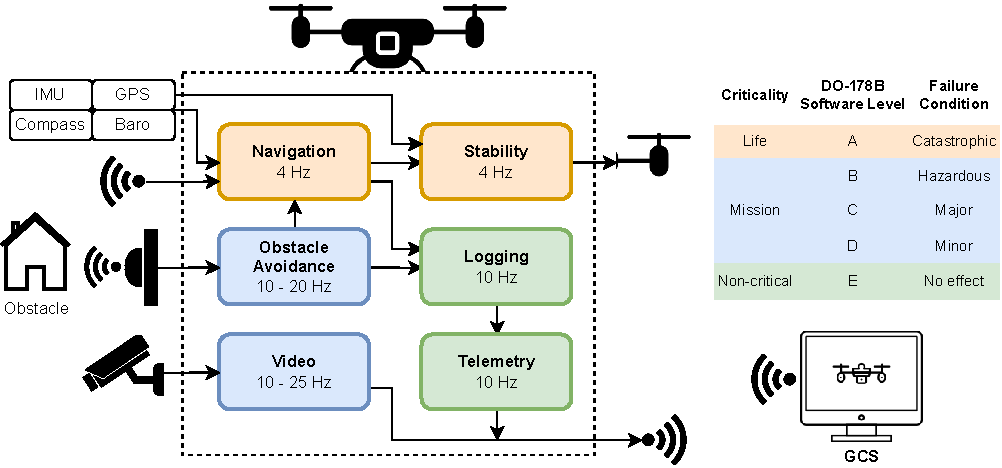
\includegraphics[width=1.0\textwidth]{./img/pdf/mcs-example} 
%   \caption[Mixed-criticality system example: UAV application]{Mixed-criticality
%     system example: UAV application (adapted from~\cite{yip_relaxing_2014}}%
%   \label{fig:mcs-example}
% \end{figure}

% % \subsection{UAV-Specific Integration Challenges}
% While \gls{mcs} principles apply across domains, \glspl{uav} face unique hurdles. They
% must meet
% extreme SWaP-C limits, where every gram needs to be justified,
% especially in the lower weight classes. \glspl{uav} fly in uncontrolled
% environments with fast changing dynamics. As it impossible to account for
% every erroneous occurrence, it must present fail-operational behavior , i.e. maintaining critical functions during faults. The
% migration to the mainstream multi-core architectures increases the complexity in
% resource sharing~\cite{burns2022mixed}.
% Current approaches force trade-offs: on one hand, multi-board provides high
% isolation but poor \gls{swap-c} metrics; on the other hand, single-board
% provides poor isolation but better \gls{swap-c}.

% % \subsection{Core Research Dichotomy}
% Two major areas of research stem from this dichotomy: a more theorethical one,
% largely focused on using criticality-specific \glspl{wcet} to schedule systems
% at each criticality level, but at the expenses of high processor utilization; a
% more practical one, focused on the safe partitioning of a system with the
% sharing of computational and communication resources, but with increased
% complexity.
% Unfortunately, the combination of both areas is not easy: flexible scheduling
% requires, at least, dynamic partitioning, whereas certified systems require
% complete separation or, at least, static partitioning~\cite{burns2022mixed}.
% This gap is acute in \glspl{uav} where both efficiency and assurance are non-negotiable.

% \subsection{Virtualization as Enabling Technology}
% \label{sec:virtualization}

\subsection{Virtualization}%
\label{sec:virtualization}
Mixed-criticality systems integrate software of disparate criticality on shared hardware.
As aforementioned,
the most promising approach is the safe partitioning of the system with shared
computation resources. This leads to concept of virtualization, a logic
abstraction of hardware resources with isolation guarantees, using different approaches such as
hypervisors, \gls{os}-level virtualization or unikernels~\cite{cinque2022virtualizing}.
%
Fig.~\ref{fig:virt-mindmap} maps the key concepts referenced in this section,
and Fig.~\ref{fig:virt-approaches-exs} illustrates representative virtualization
approaches~\cite{cinque2022virtualizing}. Starting on the left, the conventional
\gls{sw} stack runs an \gls{os} (with runtime and libraries) directly on
hardware and hosts applications. In this model, failures in any component can
propagate system-wide because no isolation layer intervenes.

\begin{figure}[!hbtp]
  \centering
  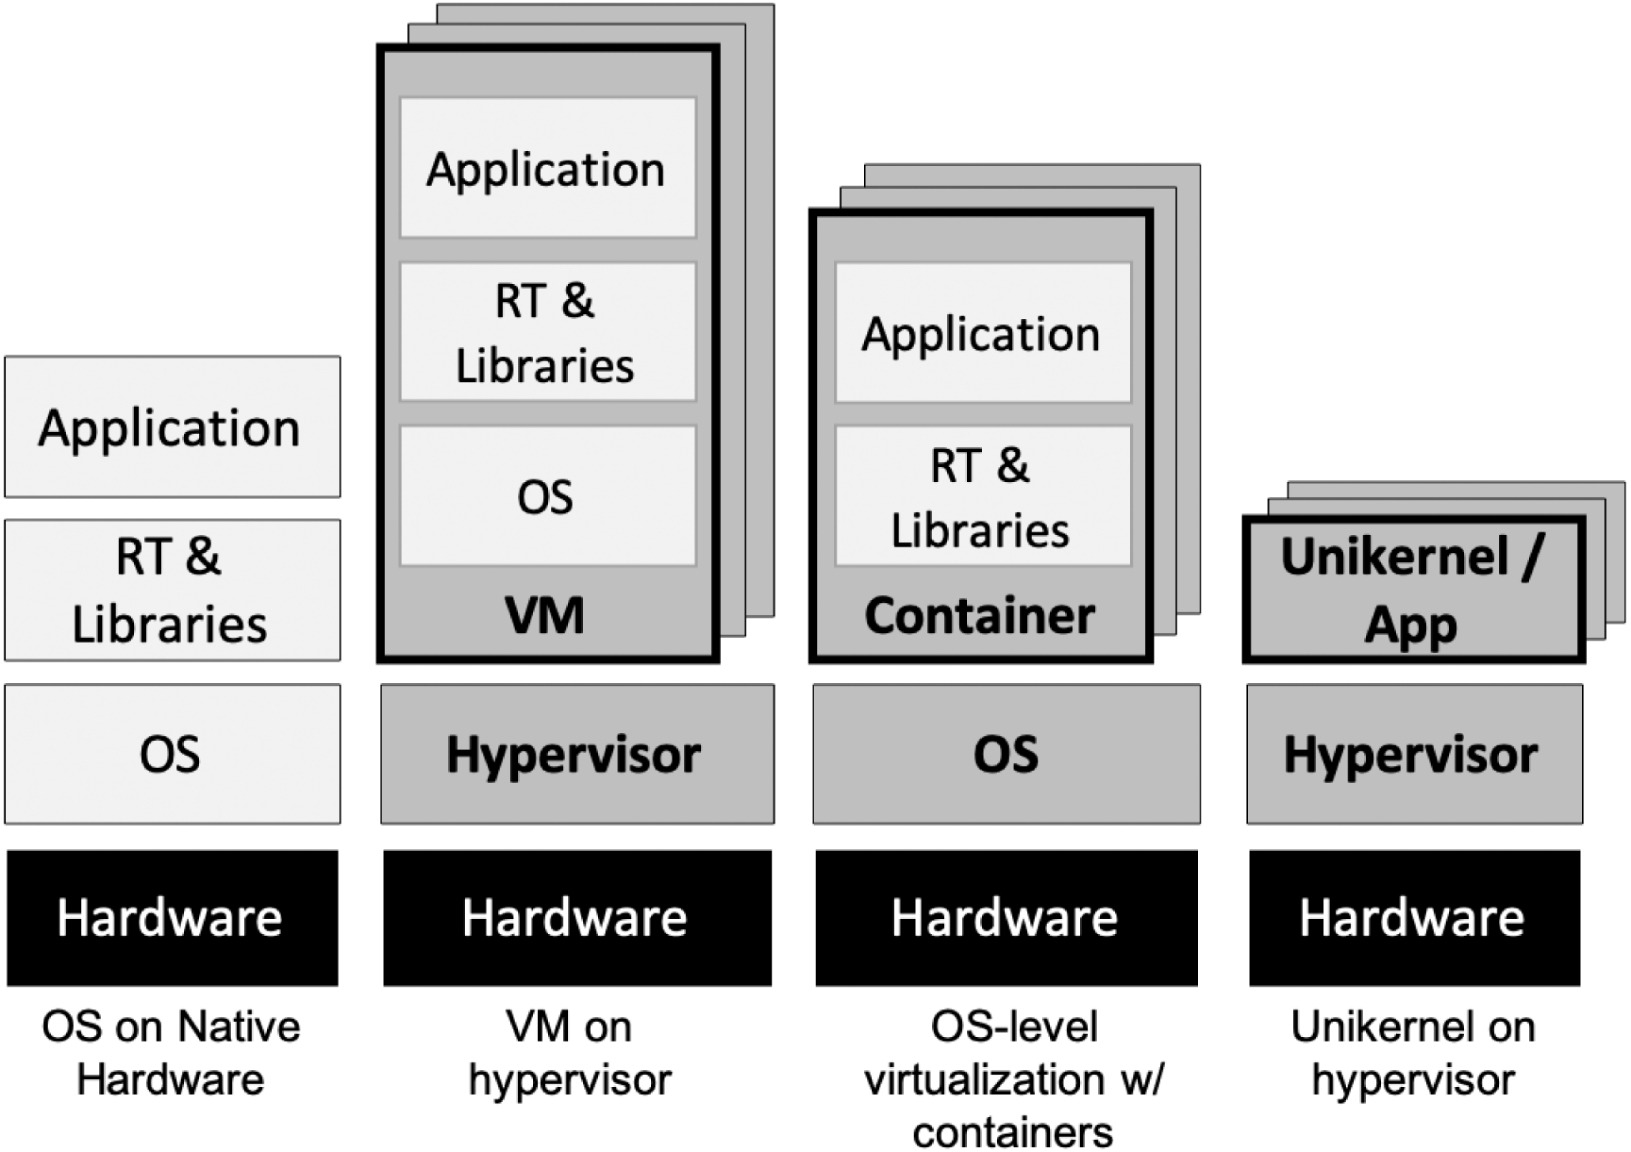
\includegraphics[width=0.6\textwidth]{./img/jpg/virt-approaches-exs} 
%  \includesvg[width=1.0\textwidth]{./img/virtualization.svg} 
  %\caption[Virtualization mind map]{Virtualization mind map}%
  \caption[Examples of virtualization approaches]{Examples of virtualization approaches~\cite{cinque2022virtualizing}\footnotemark}%
  \label{fig:virt-approaches-exs}
\end{figure}
%
\fnlicReq{Elsevier}{5457890117132}%
% \fnlicCCSA{foot:cc-lic}% CC licence

Next is hypervisor-level virtualization, which inserts a software layer that
abstracts hardware resources so multiple isolated application
environments -- \glspl{vm} or guests -- can run on the same
machine~\cite{cinque2022virtualizing}. Hypervisors are detailed in the next
section.

\gls{os}-level virtualization, or containerization, does not emulate
hardware. Popularized by
Docker~\cite{sollfrank_evaluating_2021,kumar_economically_2016}, it is widely
used in cloud settings to avoid replicating the \gls{os} stack and to increase
consolidation~\cite{cinque2022virtualizing}. A container is a process-like
domain atop the host \gls{os}, with isolated namespaces and managed resources
(\gls{cpu}, memory, filesystem, network)~\cite{cinque2022virtualizing}. Although
it lacks hardware emulation, containerization is gaining traction in \gls{rt}
contexts~\cite{xilinxRunX,struhar2020real} and in the \gls{uav} space to deploy
user-space applications on autopilots~\cite{auterion-sw-services}. Trade-offs
include sources of non-determinism (e.g., dynamic resource assignment), large
trusted code bases, and limited security hardening, which complicate testing,
assurance, and certification~\cite{cinque2022virtualizing}.

Finally, unikernel-based virtualization compiles the entire software stack
(minimal \gls{os} components, libraries, language runtime, and application) into
a single \gls{vm} image -- a unikernel or library \gls{os} -- that typically runs atop
a general-purpose hypervisor~\cite{cinque2022virtualizing}. Unikernels offer
fast boot, low memory footprint, high performance, and strong isolation (via the
host hypervisor), but they reduce flexibility: applications must target the
unikernel environment. Further work is needed for \glspl{mcs}, particularly
around certification and dependability support~\cite{cinque2022virtualizing}.

Cinque et al.~\cite{cinque2022virtualizing} relate hypervisor/guest-\gls{os}
pairings to typical use cases. General-purpose (non-\gls{rt}) hypervisors host
non-\gls{rt} guests for server consolidation, and can host \gls{rt} guests for
functional testing and prototyping (without hard guarantees). Real-time
hypervisors host non-\gls{rt} guests for \gls{qos}/performance studies and
\gls{rt} guests for safety-critical workloads. \glspl{mcs} sit in this latter
space: they require a real-time hypervisor capable of hosting both \gls{rt} and
non-\gls{rt} guests with strong isolation and bounded interference. We therefore
examine hypervisors next.

Before proceeding, we must briefly clarify a related trend in the
telecommunications domain often called ``softwarization'', which occasionally
appears in the literature under the umbrella of
virtualization~\cite{pathak_uav_2020,liu_deep_2022,nogales_adaptable_2018}.
Softwarization implements network functions that historically resided in
hardware appliances (routers, firewalls, etc.) as software running on
general-purpose servers under \glspl{vm} or
containers~\cite{kumari_taxonomy_2020}. These software instances are termed
virtual network functions (e.g., virtual firewalls, virtual
routers)~\cite{cotroneo_nfv-bench_2017}.
%
\emph{Softwarization} is also gaining traction in the \gls{uav}
field~\cite{sara_softwarization_2016,pathak_uav_2020,siddiki_abir_software-defined_2023,oubbati2020softwarization},
supporting network-centric architectures, service deployment, and communication
management, specially as systems evolve toward multi-\gls{uav}
coordination~\cite{li_distributed_2024,azari_uav--uav_2020}. However, this
approach targets the non-critical networking stacks, and therefore, falls outside the scope of our analysis.

% \begin{figure}[!hbt]
%   \centering
%   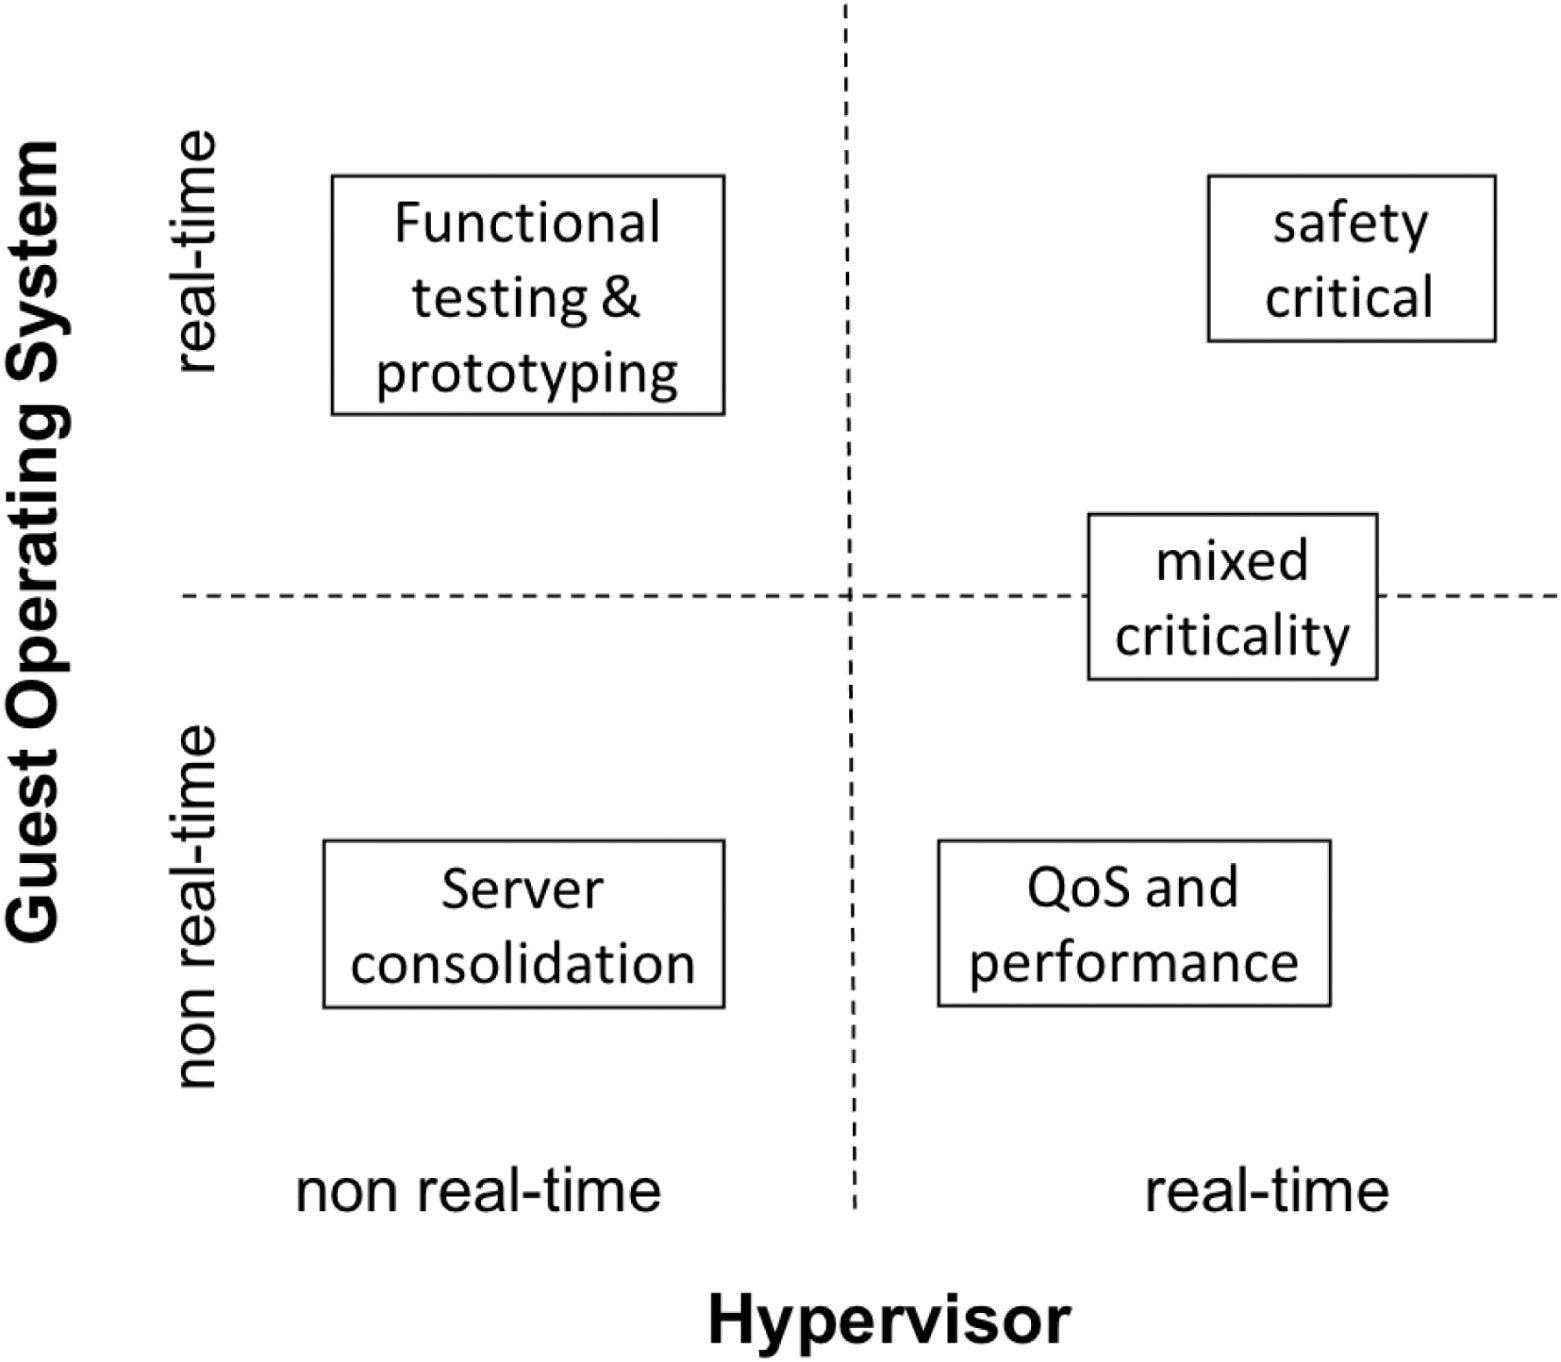
\includegraphics[width=0.6\textwidth]{./img/jpg/virt-combos} 
% %  \includesvg[width=1.0\textwidth]{./img/virtualization.svg} 
%   %\caption[Virtualization mind map]{Virtualization mind map}%
%   \caption[Hypervisor and OS combinations with related applications]{Hypervisor
%     and OS combinations with related applications~\cite{cinque2022virtualizing}\footnotemark}%
%   \label{fig:virt-combos}
% \end{figure}
% %
% \fnlicReq{Elsevier}{5457890117132}%
% % \fnlicCCSA{foot:cc-lic}% CC licence

\subsection{Hypervisors}%
\label{sec:superv--hyperv}
A hypervisor is a \glsxtrfull{vmm}: a software layer that abstracts hardware so
multiple isolated application environments -- \glspl{vm} or guests -- can run on
the same machine (see Fig.~\ref{fig:virt-approaches-exs}). Each \gls{vm}
typically includes a guest \gls{os} and its applications. To be useful in
mixed-criticality settings, the hypervisor must enforce temporal, spatial, and
fault-containment isolation~\cite{cinque2022virtualizing}. Temporal isolation means a task in one
virtual domain must not cause harmful delays to tasks in another. Spatial (memory)
isolation refers to separating code, data, and device access between domains,
generally using hardware protection (e.g., \gls{mmu}, \gls{iommu}). Fault
containment ensures that errors do not propagate to block or crash the entire
system.

Hypervisors are commonly classified by where they run, how guests interact with
them, and whether they provide explicit real-time support. Bare-metal (type~I)
hypervisors run directly on hardware and control resources themselves (e.g.,
Jailhouse~\cite{jailhouse}, Bao~\cite{martins_et_al:OASIcs:2020:11779},
CLARE~\cite{clare-home}, Xen~\cite{xen-home}).%
\footnote{Xen is typically classified as type~I (bare-metal).~\cite{cinque2022virtualizing}}
Hosted (type~II) hypervisors run atop a host \gls{os} and manage resources
indirectly (e.g., KVM~\cite{kivity2007kvm}). In fully virtualized setups the
guest runs unmodified while the hypervisor emulates privileged operations (e.g.,
KVM, Hyper-V~\cite{microsoftHyperV}); in paravirtualization the guest
cooperates with the hypervisor via hypercalls (e.g., Xen~\cite{barham2003xen}).
Real-time hypervisors add mechanisms to allocate and police time budgets so \glspl{vm}
meet timing constraints~\cite{cinque2022virtualizing}. These can be dynamic
(resources assigned at run time; e.g., KVM~\cite{kivity2007kvm}, Xen~\cite{barham2003xen})
or static (resources fixed at instantiation; e.g., Jailhouse~\cite{jailhouse}, Bao~\cite{martins_et_al:OASIcs:2020:11779}),
with static designs often preferred for \glspl{mcs} due to lower overhead, smaller
code bases, and simpler testing/certification~\cite{cinque2022virtualizing}. Hypervisors also vary by
application scope, from embedded/mission-specific to general-purpose~\cite{heiser2008role}.

Solution families reflect these choices~\cite{cinque2022virtualizing}. \emph{Separation-kernel}
hypervisors implement a small bare-metal partitioning layer that defines fixed
\glspl{vm} and information flows, delegating rich \gls{os} services and drivers to
guests (e.g., PikeOS~\cite{pikeOS}, Xtratum~\cite{masmano2009xtratum}, Jailhouse~\cite{jailhouse},
Bao~\cite{martins_et_al:OASIcs:2020:11779}). \emph{Microkernels} implement only minimal abstractions and
operations in supervisor mode (e.g., memory and thread management, \gls{ipc}), placing
drivers and higher-level services in user mode; some can serve as a hypervisor
with a user-level \gls{vmm} (e.g., seL4 with CAmkES \gls{vmm}~\cite{klein_sel4_2009,matos_sel4_2022}).
These two approaches differ in implementation focus: microkernels structure an
OS from small, user-mode components atop a minimal kernel; separation kernels
focus on static partitioning and isolation, often leveraging hardware
virtualization, and rely on guests for \gls{os}-like functionality~\cite{cinque2022virtualizing}.%

General-purpose hypervisors (e.g., KVM, Xen) can be extended with real-time
features. Some approaches leverage security \gls{cpu} extensions (e.g., Arm
TrustZone, Intel SGX) to strengthen isolation, albeit with platform dependence
(e.g., LTZVisor/RTZVisor~\cite{pinto2016towards,rtzvisor}, VOSYSMonitor~\cite{lucas2017vosysmonitor,lucas_vosysmonitor_2018}).
Unikernel solutions package a single application with minimal \gls{os} services
to run atop a hypervisor (e.g., ClickOS~\cite{martins2014clickos},
HermitCore~\cite{lankes2016hermitcore}), trading flexibility for fast boot, small footprint, and performance.

In practice, selection is guided by footprint, alignment with safety standards,
licensing, fault tolerance, security,
and hardware coverage~\cite{cinque2022virtualizing}. Cinque
et~al.~\cite{cinque2022virtualizing} provide a
broad survey of such solutions in the context of \glspl{mcs} and industrial
requirements.

% ---- Virtualization Solutions Table (no refs) ----
% Required once in your preamble:
% \usepackage{booktabs}
% \usepackage{tabularx}
% \usepackage{array}

% Required once in your preamble:
% \usepackage{booktabs}
% \usepackage{tabularx}
% \usepackage{array}

% Required once in your preamble:
% \usepackage{booktabs}
% \usepackage{tabularx}
% \usepackage{array}

% \begin{table}[!htbp]
%   \centering
%   \caption{Comparison of virtualization solutions by category, style, openness, domains, and traits}
%   \label{tab:virt-comparison}

%   \begingroup
%   \scriptsize
%   \setlength{\tabcolsep}{3pt}
%   \renewcommand{\arraystretch}{1.08}
%   \sloppy % local: avoid overfull lines inside this group

%   % Columns now: Solution | Category | Type/Style | Openness | Typical domains | Notable traits
%   \begin{tabularx}{\textwidth}{@{}
%     >{\raggedright\arraybackslash}p{0.12\textwidth}  % Solution
%     >{\raggedright\arraybackslash}p{0.12\textwidth}  % Category
%     >{\raggedright\arraybackslash}p{0.12\textwidth}  % Type / Style
%     >{\raggedright\arraybackslash}p{0.11\textwidth}  % Openness
%     >{\raggedright\arraybackslash}p{0.18\textwidth}  % Typical domains
%     >{\raggedright\arraybackslash}X                  % Notable traits (flex)
%   @{}}
%     \toprule
%     \textbf{Solution} & \textbf{Category} & \textbf{Type / Style} &
%     \textbf{Openness} & \textbf{Typical domains} &
%     \textbf{Notable traits} \\
%     \midrule

%     VxWorks MILS & Separation-kernel & Type-1, static partitioning & Commercial &
%     Avionics, safety-critical embedded &
%     Strong spatial/temporal separation; info-flow policy; minimal TCB focus \\

%     PikeOS & Microkernel (L4-based) & Type-1; mixed scheduling & Commercial &
%     Avionics &
%     ARINC653-compliance; diverse guest OSes (Android, RT-POSIX, etc.) \\

%     Xtratum & Separation-kernel / partitioning & Type-1, static, paravirtual & Dual: OSS \& commercial &
%     Avionics/space, automotive &
%     \textasciitilde9 KLOC;  not ARINC-653 complient;
%                                  multi-arch, but no ArmV8-A; runs LithOS by default \\

%     Jailhouse & Partitioning hypervisor & Type 2; Static & Open-source &
%     Embedded/industrial (ARM/x86) &
%     ``Cells'' split HW; ivshmem; small codebase; no overcommit \\

%     NOVA & Micro-hypervisor & Type-1 with tiny micro-VMM & Open-source &
%     Security-focused embedded (x86/ARMv8) &
%     \textasciitilde36 KLOC; nested paging; very low overhead in memory-bound cases \\

%     seL4 (with VMM) & Microkernel as hypervisor base & Type-1 kernel + user-space VMM & Open-source &
%     High-assurance embedded, mixed-criticality &
%     Scheduling contexts; capability model; virtualization via components \\

%     Xen (RTDS/RT-Xen) & General-purpose adapted & Type-1 (PV/PVH/HW virt) & Open-source &
%     Embedded/automotive; also cloud &
%     Real-time schedulers; dedicate pCPUs; tuned latencies in 100--200\,$\mu$s
%                                       range using PV or PVH modes\\

%     KVM (+ PREEMPT\_RT) & General-purpose adapted & Type-2 on Linux (quasi Type-1) & Open-source &
%     Automotive/industrial; cloud-edge &
%     With PREEMPT\_RT and pinning, sub-ms worst-case latencies; cgroups integration \\

%     LTZvisor / $\mu$RTZVisor & TrustZone-assisted & Monitor-mode partitioning &  Open-Source &
%     Mixed-criticality on ARM SoCs &
%     Secure/normal world split; $\mu$s-level switches; multi-guest scheduling \\

%     VOSYSmonitor & TrustZone-assisted & Monitor safety layer + GP hypervisor & Commercial &
%     Automotive (ISO 26262) &
%     Prioritized secure-world RTOS; works with Xen/KVM in normal world \\

%     ClickOS (on Xen) & Unikernel & Library-OS VMs on Type-1 & Open-source &
%     NFV / middleboxes &
%     Fast boot; tiny footprint; optimized I/O path for high throughput \\

%     HermitCore / HermiTux & Unikernel & Library-OS; bare-metal or as VM & Open-source &
%     HPC / predictable execution &
%     Low noise/latency; Linux-ABI emulation (HermiTux) for easier porting \\
%     \bottomrule
%   \end{tabularx}
%   \endgroup
% \end{table}


%\subsubsection{Bao}%
%\label{sec:bao}
%Bao (from Mandarin Chinese ``bǎohù'', meaning ``to protect'') is a security and
%safety-oriented, lightweight bare-metal hypervisor, developed by the ESRGv3 team
%at University of Minho, targeting the embedded real-time domain and especially
%the \glspl{mcs} for Armv8 and RISC-V platforms. It follows the pioneer static partioning architecture of
%\emph{Jailhouse}~\cite{jailhouse}, and improves it by discarding the need of the
%Linux Kernel to boot and manage its \glspl{vm}. From a security and
%safety perspective, this dependency compromises the system by bloating the
%system \gls{tcb} and intercepting the chain of trust in secure boot
%mechanisms~\cite{martins_et_al:OASIcs:2020:11779}. The \glspl{mcs} certification
%process is also hindered by the size of and monolithic architecture of such \glspl{os}.
%
%\emph{Jailhouse}'s breakthrough consists in a minimal software layer that
%leverages hardware-assisted virtualization technology to
%statically partition all platform resources and assign each one exclusively to a
%single \gls{vm} instance at instantiation time. The scheduler can then be
%discarded as each virtual core is statically associated to a single physical
%CPU, and the complex semantic services are relegated for the \glspl{vm}, further
%decreasing the size and complexity. It provides strong isolation and real-time
%guarantees but at the expense of efficient resource usage requirement. However,
%the Linux dependency is a liability for safety/security and performance too.
%
%Furthermore, the static partioning approach is not enough \emph{per se}, due to
%hardware resources sharing across partitions such as \glspl{llc}, interconnects,
%and memory controllers, which breach temporal isolation, hurting performance and
%determinism~\cite{bansal2018evaluating,barham2003xen}. A malicious \gls{vm} can exploit this by increasing their
%usage of a share resource (\gls{dos} attack) or by indirectly accessing other
%gls{vm}'s data thorugh the implicit timing side-channels~\cite{ge2018survey}. To tackle this
%issue, some techniques were implemented at both the OS and hypervisor level such
%as cache partioning (via locking or coloring), and memory bandwidth
%reservations~\cite{martins_et_al:OASIcs:2020:11779}.
%
%Taking this into account Bao was implemented as clean-slate
%hypervisor (see Fig.~\ref{fig:bao-arch}), comprising only a minimal thin layer of privileged software
%leveraging \gls{isa} virtualization support to implement static partioning of
%hardware resources. Its most relevant features are: memory is statically
%assigned using 2-stage translation; \gls{io} is pass-through only; 1:1 mapping
%of virtual to physical \glspl{cpu} (no scheduler required); no external
%dependencies (except for standard platform management software); provides a
%basic mecanism for inter-\gls{vm} communication; \gls{tee} support for increased
%security~\cite{martins_et_al:OASIcs:2020:11779,baoEmbeddedWorld2020}.
%
%Guest isolation is critical for a \gls{mcs}. Bao achieves complete logical
%temporal isolation due to the exclusive CPU mapping, discarding the scheduler,
%and the availability of per-\gls{cpu} architectural timers directly managed by
%the guests. Spatial isolation is provided by the 2-stage hardware virtualization
%support for the logical address space isolation. The translation overhead, page
%table and \gls{tlb} pressure is minimized using superpages, whenever
%possible, faciliting speculative fetch for potential guest performance
%improvement. A page coloring mechanism was implemented to enable \gls{llc}
%cache partioning independently for each \gls{vm}, but at the expenses of memory
%waste and fragmentation, and increased boot time~\cite{martins_et_al:OASIcs:2020:11779}.
%
%The \gls{io} are directly assigned to guests in a pass-through only
%configuration. For the memory-mapped IO architectures, as the ones supported, it
%uses the existing memory mechanism and 2-stage translation provided by the
%virtualization support to implement this for free. A peripheric can be shared
%among guests, as exclusive assignment is not checked~\cite{martins_et_al:OASIcs:2020:11779}.
%
%The interrupt virtualization support is restricted to the Arm \gls{gic}v2 and
%Arm \gls{gic}v3, which does not support direct interrupt delivery to guest
%partitions. Instead, all interrupts
%are dispatched to the hypervisor, which then must re-inject them into the guest \gls{vm} using
%a limited set of pending registers, leading to unavoidable increase in both
%interrupt latency and the complexity of interrupt management code~\cite{martins_et_al:OASIcs:2020:11779}. This was
%fixed in the newest version of the specification~\gls{gic}v4 which bypasses the hypervisor for guest interrupt delivery~\cite{dall2018design}.
%
%It is also noteworthy to mention that Xen has recently introduced
%\emph{Dom0-less}, eliminating the Linux dependency to boot and execute its
%hypervisor and \glspl{vm}. Nonetheless, Bao currently provides the same
%features but with a smaller \gls{tcb} and with clean security
%features. Moreover, and although being in its infancy, preliminary evaluation
%demonstrate only minimal virtualization overhead~\cite{martins_et_al:OASIcs:2020:11779}.
%Lastly, Bao is open-source~\cite{baoRepo} due to the developing team's strong
%belief that security requires transparency. For all the aforementioned reasons,
%Bao is the hypervisor of choice to use in this work. Tab.~\ref{tab:bao-summary}
%provides a summary of the Bao hypervisor.
%
%\emph{Bao} (from Mandarin “bǎohù,” “to protect”) is a lightweight, security- and safety-oriented bare-metal hypervisor targeting embedded real-time \glspl{mcs} on Armv8 and RISC-V. It adopts Jailhouse’s static partitioning model—exclusively assigning platform resources to guests at instantiation—while removing Jailhouse’s dependency on a Linux host, thereby shrinking the system \gls{tcb} and avoiding breaks in the secure-boot chain~\cite{jailhouse,martins_et_al:OASIcs:2020:11779}. The resulting design favors certification by minimizing code size and complexity.
%
%Bao provides strong isolation via simple, fixed resource mapping. Memory is statically assigned and enforced by two-stage translation; \gls{io} is primarily pass-through; virtual and physical \glspl{cpu} are mapped 1:1, so no scheduler is required; guests manage per-\gls{cpu} architectural timers directly. Spatial isolation leverages hardware virtualization (\gls{mmu}/\gls{iommu}); temporal isolation follows from exclusive \gls{cpu} assignment and bounded sharing. To mitigate shared-resource interference, Bao supports last-level cache partitioning via page coloring, trading some memory waste/fragmentation and longer boot time for tighter \gls{llc} control~\cite{martins_et_al:OASIcs:2020:11779}. A basic inter-\gls{vm} communication mechanism and optional \gls{tee} support complement the core.
%
%Interrupt virtualization on Arm currently relies on \gls{gic}v2/v3, which route interrupts to the hypervisor for re-injection, increasing latency and code complexity; \gls{gic}v4 addresses this by enabling direct delivery to guests~\cite{martins_et_al:OASIcs:2020:11779,dall2018design}. For \gls{io}, Bao favors direct device assignment; for memory-mapped devices, enforcement reuses the same two-stage translation. Paravirtualized I/O via \emph{VirtIO} is available for selected devices to enable efficient sharing while preserving isolation (used alongside pass-through where appropriate).
%
%Compared to contemporary options (e.g., Xen’s recent Dom0-less mode), Bao offers
%a similar static-partitioning capability with a smaller \gls{tcb} and a clean
%security posture; preliminary evaluations report minimal virtualization
%overhead~\cite{martins_et_al:OASIcs:2020:11779}. Bao is
%open-source~\cite{baoRepo}. A concise feature summary appears in
%Tab.~\ref{tab:bao-summary}.
%
%\begin{figure}[!hbt]
%  \centering
%  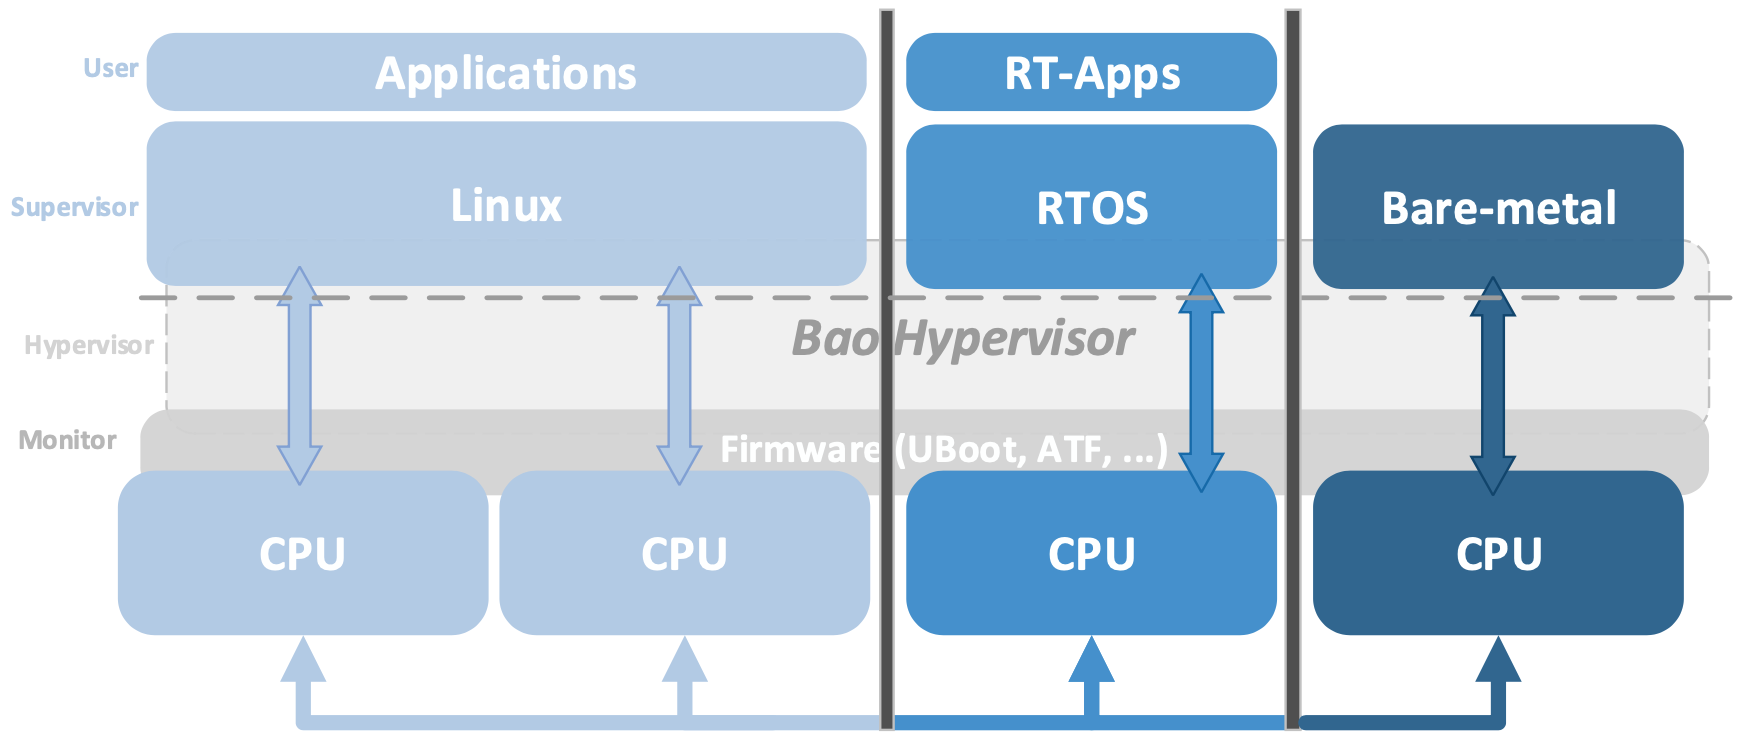
\includegraphics[width=0.7\textwidth]{./img/png/bao-arch} 
%  \caption[Hypervisor Bao architecture]{Hypervisor Bao architecture~\cite{martins_et_al:OASIcs:2020:11779}\footnotemark}%
%  \label{fig:bao-arch}
%\end{figure}
%
%\fnlicCC{foot:bao-embedded-world-lic1}%

% \subsubsection{Bao}%
% \label{sec:bao}
% \emph{Bao} (Mandarin “bǎohù,” “to protect”) is an open-source (Apache 2.0)
% lightweight, security- and safety-oriented bare-metal hypervisor for embedded real-time \glspl{mcs}, developed by the ESRGv3 team at the University of Minho~\cite{martins_et_al:OASIcs:2020:11779,baoRepo}. It
% follows the static, type-I partitioning model pioneered by
% \emph{Jailhouse}~\cite{jailhouse} but removes the Linux host dependency,
% reducing the system \gls{tcb} -- currently around 8 kLOC C + 500 ASM --  and
% easing the path towards certification~\cite{martins_et_al:OASIcs:2020:11779}.
% It supports the Armv7/8-A and -R, the RISCV RV32 and R64
% platforms. Additionally, an ongoing effort is providing support for the Infineon
% Tricore 1.8 and Renesas RH850. A concise summary appears
% in Table~\ref{tab:bao-summary}.

% Bao is a clean-slate design (Fig.~\ref{fig:bao-arch}) comprising a thin
% privileged layer that leverages \gls{isa} virtualization for static
% partitioning~\cite{martins_et_al:OASIcs:2020:11779}.
% It has no scheduler and does not rely on external libraries or privileged
% \gls{vm} (e.g.,~Linux), as Jailhouse does~\cite{jailhouse}, depending only on the standard
% platform-management firmware to initialize the system~\cite{martins_et_al:OASIcs:2020:11779} and
% perform platform-specific tasks. By removing the Linux dependency, it improves
% the safety/security guarantees and real-time performance~\cite{martins_et_al:OASIcs:2020:11779}.

% Bao is specifically targetted for safety-critical applications, such as a
% \gls{mcs}, by providing temporal, spatial, and fault containment isolation.
% Temporal isolation is achieved by precluding the scheduler, enforcing exclusive 
% 1:1 mapping between virtual and physical \glspl{cpu} at \gls{vm} instantiation
% time, and by enabling guest access and management to per-\gls{cpu} architectural
% timers.
% Memory is statically assigned and enforced via two-stage
% translation, and superpages are used when possible to reduce translation and
% \gls{tlb} pressure and aid speculative fetch, providing spatial isolation.
% %
% While this yields strong isolation and
% real-time guarantees, shared hardware (e.g., \glspl{llc}, interconnects, memory
% controllers) can still create temporal interference and exposure to \gls{dos}
% and timing side
% channels~\cite{bansal2018evaluating,barham2003xen,ge2018survey}. Accordingly,
% Bao employs cache partitioning coloring and memory-bandwidth to mitigate this issue.

% For devices, Bao favors direct assignment (pass-through). For memory-mapped
% \gls{io}, the same two-stage translation used for memory protection applies;
% exclusivity is not enforced automatically, so deployments must avoid unintended
% sharing~\cite{martins_et_al:OASIcs:2020:11779}. Paravirtualized I/O via
% \emph{VirtIO} is available for selected
% devices~\cite{costa2022virtio,ribeiro2023virtio,rocha_mitigating_2023,peixoto-virtio-2024,baoRepo},
% enabling efficient sharing while preserving isolation and complementing
% pass-through where appropriate.
% Also on the topic of sharing, Bao offers a basic inter-\gls{vm} communication
% mechanism, using shared memory~\cite{martins_et_al:OASIcs:2020:11779,baoEmbeddedWorld2020}.

% Interrupt virtualization currently targets Arm \gls{gic}v2/v3,
% which route interrupts to the hypervisor for re-injection, which adds latency
% and code complexity~\cite{martins_et_al:OASIcs:2020:11779}. \gls{gic}v4 solves
% this problem by enabling direct guest delivery~\cite{dall2018design}, but its prevalence is still reduced, so this problem is expected to be addressed as it gains more market adoption. On the open standard RISC-V, Bao supports both
% \gls{plic} and the more recent \gls{aia}~\cite{marques_interrupting_2024,baoRepo}.

% Compared with contemporaries (e.g., Xen’s Dom0-less mode), Bao offers similar
% static partitioning with a smaller \gls{tcb} and a clean security posture, with minimal virtualization
% overhead~\cite{martins_et_al:OASIcs:2020:11779}.
% Lastly, Bao has been extensively benchmarked using the standard MiBench
% \gls{aics} suite, targeted for real-time embedded applications such as
% automotive and industrial. The results indicate minimal virtualization
% overhead and that cache coloring, although not
% optimal, can effectively mitigate the inter-\gls{vm}
% interference~\cite{martins2023shedding}.

% The Bao hypervisor presents itself as a perfect solution to build a trustworthy
% open-source reference software stack for \gls{uav} applications due to its
% open-source nature, strict domain isolation with efficient resource sharing, and
% extensive benchmarking, paving the way for the consolidation of the
% mixed-criticality software stacks into a single hardware platform, while
% minimizing the \gls{swap-c} metrics.

% \begin{figure}[!hbt]
%   \centering
%   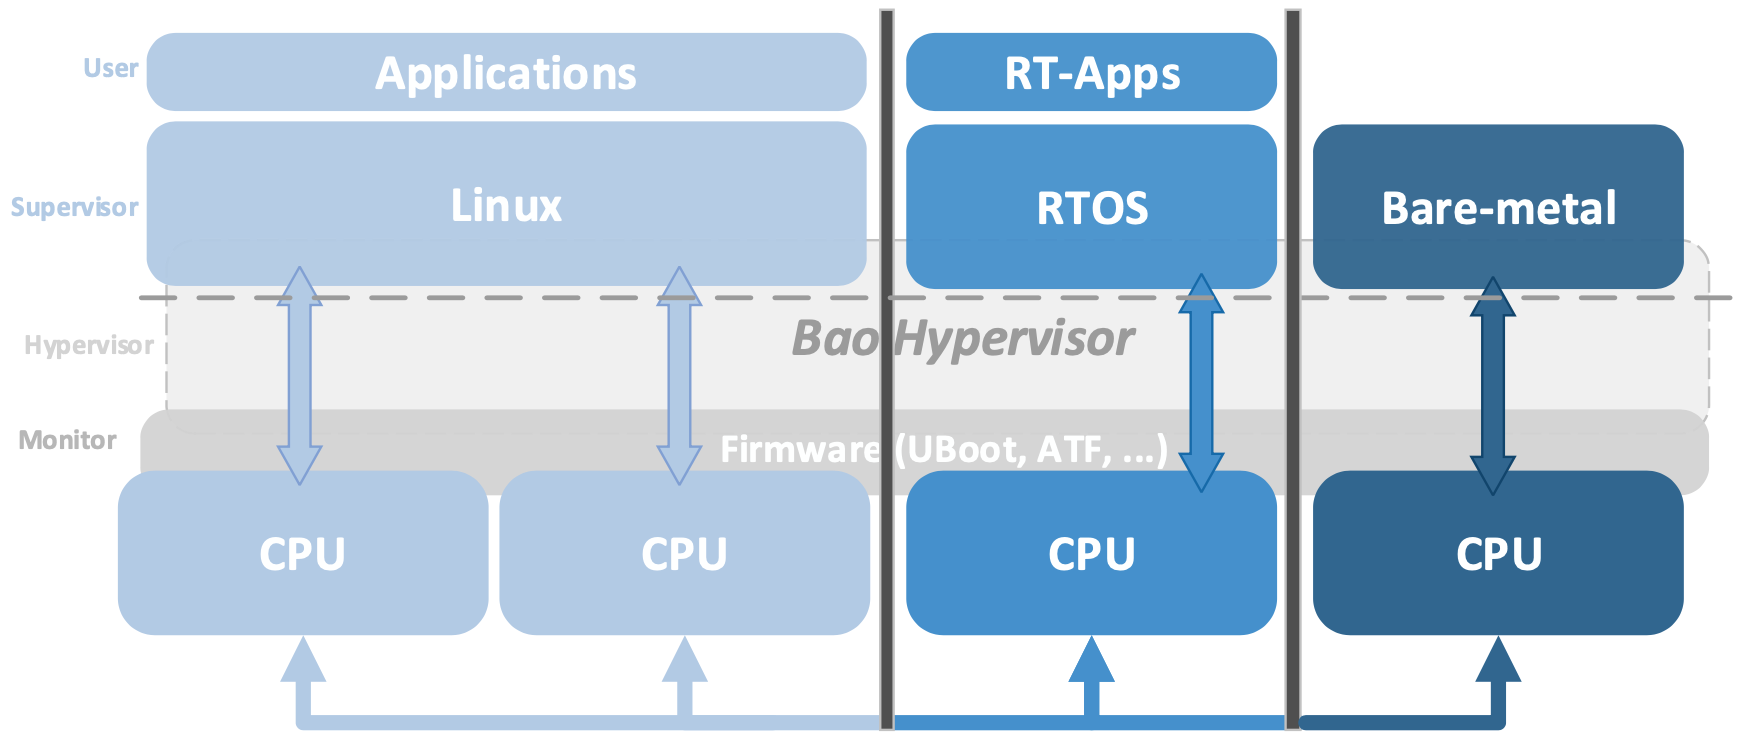
\includegraphics[width=0.7\textwidth]{./img/png/bao-arch}
%   \caption[Hypervisor Bao architecture]{Hypervisor Bao architecture~\cite{martins_et_al:OASIcs:2020:11779}\footnotemark}%
%   \label{fig:bao-arch}
% \end{figure}
% \fnlicCC{foot:bao-embedded-world-lic1}%

\subsubsection{Bao}%
\label{sec:bao}
\emph{Bao} (Mandarin “bǎohù,” “to protect”) is an open-source, lightweight,
security- and safety-oriented bare-metal hypervisor for embedded real-time
\glspl{mcs}, developed by the ESRGv3 team at the University of
Minho~\cite{martins_et_al:OASIcs:2020:11779,baoRepo}. It follows the static,
type-I partitioning model pioneered by \emph{Jailhouse}~\cite{jailhouse} but
removes the Linux host dependency, thereby reducing the system
\gls{tcb}—currently around $\sim$8\,kLOC of C plus $\sim$500\,LOC of
assembly—and easing the path toward
certification~\cite{martins_et_al:OASIcs:2020:11779}. Bao supports Armv7/8-A and
-R and RISC-V (RV32 and RV64), with ongoing work toward Infineon TriCore~1.8 and
Renesas RH850.

Bao is a clean-slate design (Fig.~\ref{fig:bao-arch}) comprising a thin
privileged layer that leverages \gls{isa} virtualization for static
partitioning~\cite{martins_et_al:OASIcs:2020:11779}. It has no scheduler and
does not rely on external libraries or a privileged \gls{vm} (e.g., Linux), in
contrast to Jailhouse~\cite{jailhouse}, depending only on standard
platform-management firmware to initialize the system and perform
platform-specific tasks~\cite{martins_et_al:OASIcs:2020:11779}. Removing the
Linux dependency improves safety/security guarantees and real-time
performance~\cite{martins_et_al:OASIcs:2020:11779}.

\begin{figure}[!hbtp]
  \centering
  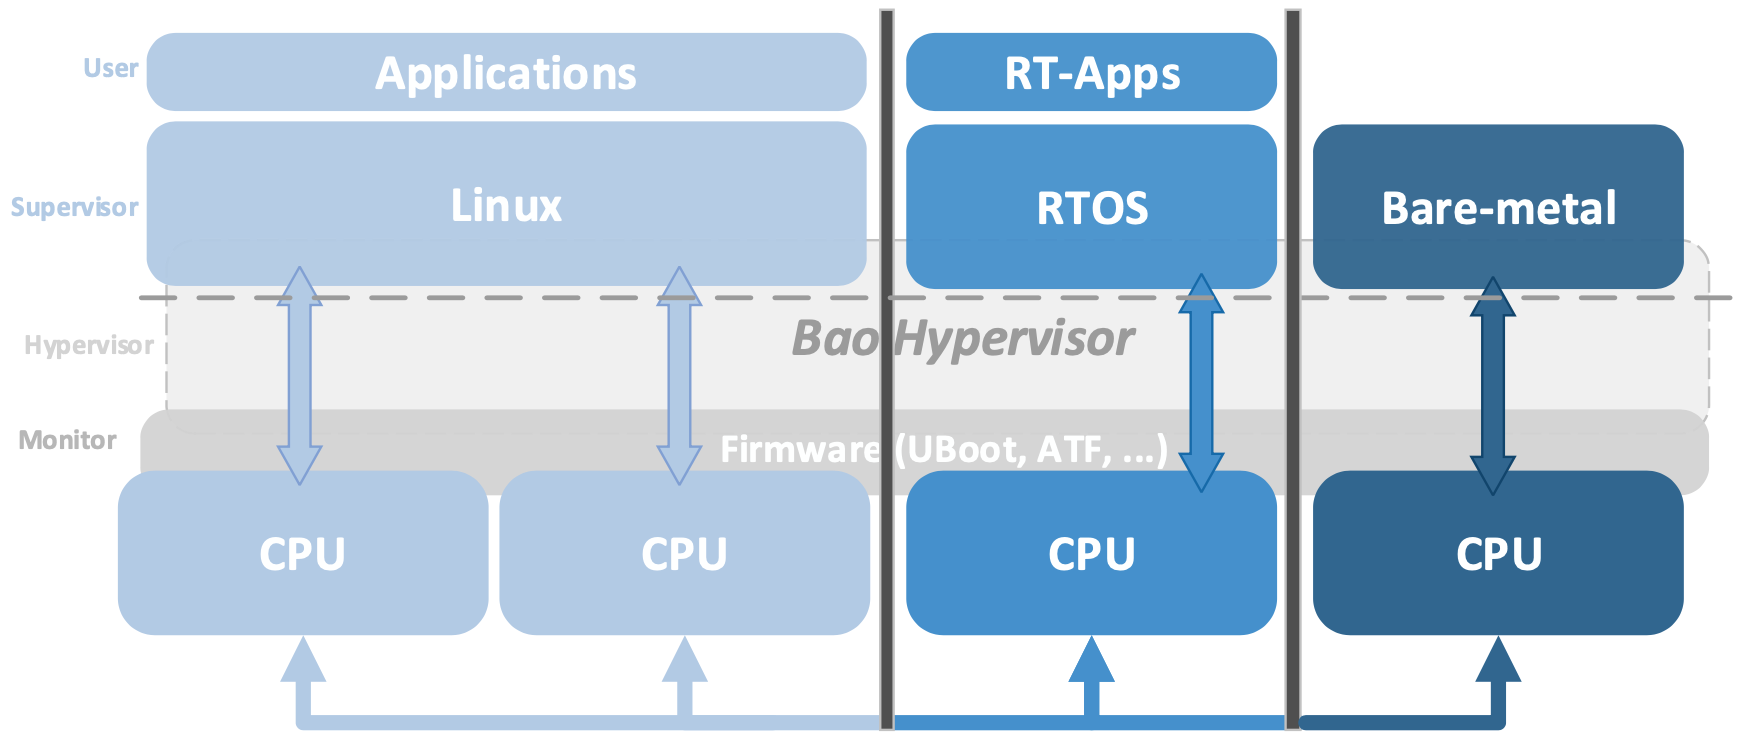
\includegraphics[width=0.7\textwidth]{./img/png/bao-arch}
  \caption[Hypervisor Bao architecture]{Hypervisor Bao architecture~\cite{martins_et_al:OASIcs:2020:11779}\footnotemark}%
  \label{fig:bao-arch}
\end{figure}
\fnlicCC{foot:bao-embedded-world-lic1}%

Bao targets safety-critical systems, such as \glspl{mcs}, by providing
temporal, spatial, and fault-containment isolation~\cite{martins_et_al:OASIcs:2020:11779}. Temporal isolation follows
from the absence of a scheduler and the exclusive 1:1 mapping between virtual
and physical \glspl{cpu} at \gls{vm} instantiation time, together with guest
access and management of per-\gls{cpu} architectural timers~\cite{martins_et_al:OASIcs:2020:11779}. Spatial isolation is ensured by
statically assigned memory enforced via two-stage translation, using superpages
when possible to reduce translation and \gls{tlb} pressure and to aid
speculative fetch~\cite{martins_et_al:OASIcs:2020:11779}. While these mechanisms provide strong isolation and real-time
behavior, shared hardware resources (e.g., \glspl{llc}, interconnects, memory
controllers) can still induce temporal interference and expose \glspl{vm} to
\gls{dos} and timing side
channels~\cite{bansal2018evaluating,barham2003xen,ge2018survey}. To mitigate
these effects, Bao employs cache coloring for \gls{llc} partitioning and
memory-bandwidth regulation~\cite{martins_et_al:OASIcs:2020:11779}.

For devices, Bao favors direct assignment (pass-through). For memory-mapped
\gls{io}, the same two-stage translation used for memory protection applies;
exclusivity is not enforced automatically, so deployments must avoid unintended
sharing~\cite{martins_et_al:OASIcs:2020:11779}. Paravirtualized I/O via
\emph{VirtIO} is available for selected
devices~\cite{costa2022virtio,ribeiro2023virtio,rocha_mitigating_2023,peixoto-virtio-2024,baoRepo},
enabling efficient sharing while preserving isolation and complementing
pass-through where appropriate. Bao also offers a basic inter-\gls{vm}
communication mechanism via shared
memory~\cite{martins_et_al:OASIcs:2020:11779,baoEmbeddedWorld2020}.
%
Interrupt virtualization currently targets Arm \gls{gic}v2/v3, which route
interrupts to the hypervisor for re-injection, adding latency and code
complexity~\cite{martins_et_al:OASIcs:2020:11779}. Arm \gls{gic}v4 addresses
this with direct guest delivery~\cite{arm-gicv4,dall2018design}, though adoption
is still limited. On
RISC-V, Bao supports both the legacy \gls{plic} and the more recent
\gls{aia}~\cite{marques_interrupting_2024,baoRepo}.

Relative to the alternatives (e.g., Xen’s Dom0-less mode), Bao offers a similar
static-partitioning model with a smaller \gls{tcb} and a clean security posture,
with minimal virtualization
overhead~\cite{martins_et_al:OASIcs:2020:11779}. Furthermore, Bao
has been extensively benchmarked with the MiBench \gls{aics} suite for real-time
embedded domains (e.g., automotive and industrial), showing minimal overhead and
demonstrating that cache coloring, although not optimal, can effectively
mitigate inter-\gls{vm} interference~\cite{martins2023shedding}.

Overall, Bao is a suitable foundation for a trustworthy open-source reference
software stack for \gls{uav} applications: it is open-source, enforces strict
domain isolation with efficient resource sharing, and has undergone extensive
benchmarking, enabling consolidation of mixed-criticality software on a single
hardware platform while minimizing \gls{swap-c}.
Table~\ref{tab:bao-summary} presents a concise summary on the Bao hypervisor.


% \begin{table}[!hbtp]
%   \caption[Bao hypervisor summary]{Bao hypervisor summary~\cite{baoRepo}}

% Please add the following required packages to your document preamble:
% \usepackage{multirow}
% \usepackage{graphicx}
% \usepackage[table,xcdraw]{xcolor}
% Beamer presentation requires \usepackage{colortbl} instead of \usepackage[table,xcdraw]{xcolor}
% Please add the following required packages to your document preamble:
% \usepackage{multirow}
% \usepackage{graphicx}
% \usepackage[table,xcdraw]{xcolor}
% Beamer presentation requires \usepackage{colortbl} instead of \usepackage[table,xcdraw]{xcolor}
\begin{table}[!hbtp]
\caption[Bao hypervisor summary]{Bao hypervisor summary~\cite{baoRepo}}
\label{tab:bao-summary}
\resizebox{\columnwidth}{!}{%
\begin{tabular}{lllll}
\hline
{\color[HTML]{000000} \textbf{Architecture}} &
  {\color[HTML]{000000} \textbf{Supported platforms}} &
  {\color[HTML]{000000} \textbf{Size}} &
  {\color[HTML]{000000} \textbf{License}} &
  {\color[HTML]{000000} \textbf{Version}} \\ \hline
{\color[HTML]{000000} \begin{tabular}[c]{@{}l@{}}Type I,\\ Static\end{tabular}} &
  {\color[HTML]{000000} \begin{tabular}[c]{@{}l@{}}Armv7/8-A, Armv7/8-R\\ RISC-V RV32 and RV64\\ Infineon Tricore 1.8 (WIP)\\ Renesas RH850 (WIP)\end{tabular}} &
  {\color[HTML]{000000} \begin{tabular}[c]{@{}l@{}}Small \\ $\sim$8 kLOC C +\\ $\sim$500 LOC ASM\end{tabular}} &
  {\color[HTML]{000000} Apache 2.0} &
  {\color[HTML]{000000} 1.0} \\ \hline
{\color[HTML]{000000} \textbf{Features}} &
  \multicolumn{4}{c}{{\color[HTML]{000000} \textbf{Isolation}}} \\ \hline
{\color[HTML]{000000} Static partioning} &
  \multicolumn{2}{l}{{\color[HTML]{000000} \textbf{Spatial}}} &
  \multicolumn{2}{l}{{\color[HTML]{000000} \textbf{Temporal}}} \\ \cline{2-5} 
{\color[HTML]{000000} IO pass-through and VirtIO support} &
  \multicolumn{2}{l}{{\color[HTML]{000000} }} &
  \multicolumn{2}{l}{{\color[HTML]{000000} }} \\
{\color[HTML]{000000} \begin{tabular}[c]{@{}l@{}}1:1 mapping of virtual to physical CPUs \\ (no scheduler required)\end{tabular}} &
  \multicolumn{2}{l}{\multirow{-2}{*}{{\color[HTML]{000000} \begin{tabular}[c]{@{}l@{}}Provided by a 2-stage translation \\ HW virtualization support\end{tabular}}}} &
  \multicolumn{2}{l}{\multirow{-2}{*}{{\color[HTML]{000000} \begin{tabular}[c]{@{}l@{}}Exclusive CPU assignment \\ discards the scheduler\end{tabular}}}} \\
{\color[HTML]{000000} \begin{tabular}[c]{@{}l@{}}Virtual interrupts directly mapped \\ to physical ones\end{tabular}} &
  \multicolumn{2}{l}{{\color[HTML]{000000} }} &
  \multicolumn{2}{l}{{\color[HTML]{000000} }} \\
 &
  \multicolumn{2}{l}{{\color[HTML]{000000} }} &
  \multicolumn{2}{l}{{\color[HTML]{000000} }} \\
 &
  \multicolumn{2}{l}{{\color[HTML]{000000} }} &
  \multicolumn{2}{l}{{\color[HTML]{000000} }} \\
\multirow{-3}{*}{\begin{tabular}[c]{@{}l@{}}No external dependencies (except for \\ standard platform management firmware)\end{tabular}} &
  \multicolumn{2}{l}{\multirow{-5}{*}{{\color[HTML]{000000} \begin{tabular}[c]{@{}l@{}}Translation overhead is minimized using \\ superpages whenever possible, faciliting \\ speculative fetch for potential guest \\ performance improvement\end{tabular}}}} &
  \multicolumn{2}{l}{{\color[HTML]{000000} }} \\
{\color[HTML]{000000} } &
  \multicolumn{2}{l}{{\color[HTML]{000000} }} &
  \multicolumn{2}{l}{{\color[HTML]{000000} }} \\
\multirow{-2}{*}{{\color[HTML]{000000} \begin{tabular}[c]{@{}l@{}}Provides a basic mecanism for inter-VM \\ communication\end{tabular}}} &
  \multicolumn{2}{l}{{\color[HTML]{000000} }} &
  \multicolumn{2}{l}{{\color[HTML]{000000} }} \\
{\color[HTML]{000000} } &
  \multicolumn{2}{l}{{\color[HTML]{000000} }} &
  \multicolumn{2}{l}{{\color[HTML]{000000} }} \\
\multirow{-2}{*}{{\color[HTML]{000000} \begin{tabular}[c]{@{}l@{}}State-of the art partioning mechanisms to \\ be implemented (e.g., memory throttling)\end{tabular}}} &
  \multicolumn{2}{l}{\multirow{-4}{*}{{\color[HTML]{000000} \begin{tabular}[c]{@{}l@{}}It uses cache coloring to enable LLC cache \\ partioning independently for each VM, but \\ at the expenses of memory waste and \\ fragmentation and increased boot time\end{tabular}}}} &
  \multicolumn{2}{l}{\multirow{-8}{*}{{\color[HTML]{000000} \begin{tabular}[c]{@{}l@{}}Per-CPU architecture timers \\ are available to and directly \\ managed by the guests\end{tabular}}}} \\ \hline
{\color[HTML]{000000} \textbf{IO}} &
  \multicolumn{2}{l}{{\color[HTML]{000000} \textbf{Interrupts}}} &
  \multicolumn{2}{l}{{\color[HTML]{000000} \textbf{Related Work}}} \\ \hline
{\color[HTML]{000000} } &
  \multicolumn{2}{l}{{\color[HTML]{000000} }} &
  \multicolumn{2}{l}{{\color[HTML]{000000} }} \\
{\color[HTML]{000000} } &
  \multicolumn{2}{l}{{\color[HTML]{000000} }} &
  \multicolumn{2}{l}{{\color[HTML]{000000} }} \\
\multirow{-3}{*}{{\color[HTML]{000000} \begin{tabular}[c]{@{}l@{}}Directly assigned to guest in a \\ pass-through only IO configuration\end{tabular}}} &
  \multicolumn{2}{l}{\multirow{-3}{*}{{\color[HTML]{000000} \begin{tabular}[c]{@{}l@{}}Supports Arm GICv2 and GICv3\\ Supports RISC-V PLIC and AIA\end{tabular}}}} &
  \multicolumn{2}{l}{\multirow{-3}{*}{{\color[HTML]{000000} \begin{tabular}[c]{@{}l@{}}Jailhouse: pioneer in the static \\ partioning adopted by Bao but \\ requires the Linux Kernel to boot\end{tabular}}}} \\
{\color[HTML]{000000} } &
  \multicolumn{2}{l}{{\color[HTML]{000000} }} &
  \multicolumn{2}{l}{{\color[HTML]{000000} }} \\
{\color[HTML]{000000} } &
  \multicolumn{2}{l}{{\color[HTML]{000000} }} &
  \multicolumn{2}{l}{{\color[HTML]{000000} }} \\
{\color[HTML]{000000} } &
  \multicolumn{2}{l}{{\color[HTML]{000000} }} &
  \multicolumn{2}{l}{{\color[HTML]{000000} }} \\
{\color[HTML]{000000} } &
  \multicolumn{2}{l}{{\color[HTML]{000000} }} &
  \multicolumn{2}{l}{{\color[HTML]{000000} }} \\
\multirow{-5}{*}{{\color[HTML]{000000} \begin{tabular}[c]{@{}l@{}}For memory-mapped IO it uses the existing \\ memory mechanism and 2-stage translation \\ provided by the virtualization support\end{tabular}}} &
  \multicolumn{2}{l}{\multirow{-5}{*}{{\color[HTML]{000000} \begin{tabular}[c]{@{}l@{}}Interrupts are forwarded to the hypervisor \\ which must re-inject them in the VM using \\ a limited set of pending registers\end{tabular}}}} &
  \multicolumn{2}{l}{\multirow{-5}{*}{{\color[HTML]{000000} \begin{tabular}[c]{@{}l@{}}Xen Dom0-less: eliminates the \\ Linux dependency to boot and \\ execute\end{tabular}}}} \\
{\color[HTML]{000000} } &
  \multicolumn{2}{l}{{\color[HTML]{000000} }} &
  \multicolumn{2}{l}{{\color[HTML]{000000} }} \\
{\color[HTML]{000000} } &
  \multicolumn{2}{l}{{\color[HTML]{000000} }} &
  \multicolumn{2}{l}{{\color[HTML]{000000} }} \\
{\color[HTML]{000000} } &
  \multicolumn{2}{l}{{\color[HTML]{000000} }} &
  \multicolumn{2}{l}{{\color[HTML]{000000} }} \\
{\color[HTML]{000000} } &
  \multicolumn{2}{l}{{\color[HTML]{000000} }} &
  \multicolumn{2}{l}{{\color[HTML]{000000} }} \\
\multirow{-5}{*}{{\color[HTML]{000000} \begin{tabular}[c]{@{}l@{}}Paravirtualized I/O via VirtIO is supported \\ for selected devices, enabling efficient \\ sharing with isolation\end{tabular}}} &
  \multicolumn{2}{l}{\multirow{-5}{*}{{\color[HTML]{000000} }}} &
  \multicolumn{2}{l}{\multirow{-5}{*}{{\color[HTML]{000000} \begin{tabular}[c]{@{}l@{}}Bao provides basically the same \\ features from the previous ones, \\ but has a smaller TCB and \\ implements clean security features\end{tabular}}}} \\ \hline
\end{tabular}%
}
\end{table}

\section{Unmanned Aerial Vehicles}%
\label{sec:unmann-aeri-vehicl}
\glsxtrfull{uav}s, \glsxtrfull{uas}, or more commonly drones, are a class of
unmanned robotic vehicles that can execute flying missions and carry payloads,
guided either by remote control stations or in an autonomous
way~\cite{alladi2022UAVBlockain,glossner2021overview}.
They belong to a broader class of \glspl{uv}, alongside with \glspl{ugv}, \glspl{usv}
(e.g., boats) and \glspl{uuv}~\cite{glossner2021overview}.

\glspl{uav} date back to as far as the 18\textsuperscript{th} century. In 1783,
France, the first uncrewed aircraft -- a hot air balloon --
was publicly displayed~\cite{uavHistory}. In 1896, Alfred Nobel created the first camera-based \gls{uav}
(rocket) and launched it. In 1935, U.K., the first modern \gls{uav} was
developed, a low cost radio controlled aircraft. The term \emph{drone} was
presumably coined by Lieutenant Commander Fahrney, who as in charge of U.S. Navy
program \emph{Radio Controlled Aircraft}~\cite{uavHistory}. The first \gls{uav} designed for
surveillance and scouting was developed in 1973 in Israel, and the \emph{Gulf
  War} was the first conflict utilizing \glspl{uav}. Starting from 2003,
the \gls{uav} commercial market started to emerge with the release of the
\emph{Amazon Prime}~\cite{alladi2022UAVBlockain}.
However, it was until 2006 that the \glspl{uav} were first
permitted in the U.S. civilian space. More recently, in 2010, the first
smartphone controlled quadcopter was developed, and in 2013 camera equipped
\glspl{uav} entered the consumer market~\cite{uavHistory}.

From then on, the selling price dropped significantly, alongside with the
emergence of some of the first open-source projects on \gls{uav} control --
Paparazzi UAS in 2003~\cite{paparazzi-home}, ArduPilot in
2008~\cite{arduPilotHistory} and Dronecode~\cite{px4History} (now PX4) in 2011
-- led to a boom in the commercial \gls{uav} market. In 2017 the North America
market had a revenue of 737 million USD dollars and a eight-fold increase is
expected for 2026 with a staggering 6.7 billion USD dollars, with strong
contributions from the sectors of agriculture and farming, and security and law enforcement~\cite{mohsan2022towards}.

The versatility and utility of \glspl{uav} are well displayed is by its wide
range of applications, performing tasks with high added value and that would be
somewhat hard or impossible for a person to achieve~\cite{silvagni_multipurpose_2017,lammers_airborne_2023}: rescue operations and
saving lifes~\cite{silvagni_multipurpose_2017}, agriculture~\cite{tsouros_review_2019}, pipeline
inspections~\cite{yu_uav-based_2022}, delivering goods and medical supplies~\cite{lammers_airborne_2023}, video capturing and
surveillance~\cite{dilshad_applications_2020}, cartography~\cite{caroti_uav-borne_2017},
among others.

However, only recently regulations have been explicitly enforced on \glspl{uav},
with many countries allowing drones to fly over populated areas (at altitudes
lower than 150 m)~\cite{nassi2021sok}. For example, in 2019, the E.U.~stated that all drones under
25 kgs are able to fly without prior authorization under some constraints. On
the other hand, it imposed that all drones must register in their respective
states, and that each state must define no-fly zones where drones are
forbidden to enter~\cite{Ullah2020UAV5gEULegisl}.
%
Yet, global standardization remains absent. In 2020, the \gls{faa}, together with \gls{nasa} and other agencies, released \gls{utm}~2.0, which describes protocols to enable multiple \gls{bvlos} operations within shared airspace~\cite{glossner2021overview}.

Broadly, five categories frame \gls{uav}
regulation~\cite{fotouhi2019UAVCellularCommSurvey,stocker2017UAVRegulationsReview}. First,
\emph{applicability} defines the scope of the rules—typically by vehicle type, weight,
and intended role. Second, \emph{operational limitations} constrain where and how
\glspl{uav} may fly (e.g., airspace classes, altitude limits, proximity to
people or infrastructure). Third, \emph{administrative and legal requirements}
establish oversight mechanisms such as registration, licensing, and
record-keeping. Fourth, \emph{technology specifications and requirements} address
mechanical integrity and the communications/control capabilities needed for safe
operation (e.g., command-and-control links, geofencing, fail-safes). Finally,
\emph{moral and ethics} considerations focus on privacy and the broader security
of people and communities.

%\enlargethispage{\baselineskip}
% \clearpage % or \newpage


\subsection{Classification}%
\label{sec:classification}
An \gls{uav} can be classified in multiple ways:
\begin{itemize}
\item \textbf{Flight principles}: \glspl{uav} can be lighter
  than air, e.g., a balloon or a blimp, such as the EBlimp Atom~\cite{eblimp-atom}, if it uses a motorized propulsion
  system. On the other hand, if they are heavier than air, they are named
  gliders~\cite{px4-glider}, rotor-crafts~\cite{energyorDrone}, and birds~\cite{drone-bird}.
 % 
\item \textbf{Airframe}: The most visible external feature of a \gls{uav} is its
  airframe, classified as fixed-wing, fixed-wing hybrid, single rotor, and
  multirotor~\cite{mohsan2022towards}.
  Fixed-wing
  platforms are the fastest and are typically used in power-line inspection and
  They carry heavier payloads, and offer longer endurance, but they require
  runway takeoff and landing~\cite{mohsan2022towards}.
The hybrid variant addresses the runway limitation by enabling \gls{vtol} like a
rotorcraft while cruising like a fixed-wing.
  They have a larger autonomy, but are slower~\cite{mohsan2022towards}.
  Rotor-crafts -- single-rotor and multirotor -- can hover and perform
  \gls{vtol}. They offer good endurance but are expensive,
  require skilled operators, and are mechanically complex and
  vibration-prone~\cite{mohsan2022towards}. Multirotors (e.g., tricopters,
  quadcopters, hexacopters and octocopters)
  are the most affordable and widely
  produced, but they usually have shorter autonomy due to higher power
  consumption~\cite{mohsan2022towards}.
 % 
\item \textbf{Altitude}: Broadly, \glspl{uav} are divided into \glspl{lap} and
  \glspl{hap}. A \gls{lap} maximum altitude ranges from 3 to 9 kms and is
  typically used to support cellular communications. \glspl{hap}, on the other
  hand, are deployed above the 9 km altitude and are used to support cellular
  communication but with wider coverage, endorsed by companies such as Google
  and Facebook~\cite{mohsan2022towards}.
%  
\item \textbf{Overall weight}: \glspl{uav} can have few grams of weight or
  hundreds of kilograms. For example, Australia labels them as \emph{micro}
  (below 100 g),
  \emph{very small} (from 100 g to 2 kg), \emph{small} (from 2 to 25 kgs),
  \emph{medium} (from 25 to 150 kgs), and \emph{large} (over
  150 kgs)~\cite{alladi2022UAVBlockain}.
%  
\item \textbf{Power source}: \glspl{uav} can be powered using electricity,
  fuel, or a hybrid solution. Except for the fuel-only powered ones (e.g., Nitro
  Stingray, and Goliath Quadcopter~\cite{gasPoweredDrone}), all the
  others use electric motors. These motors can be powered through batteries
  (e.g., Parrot\cite{parrotDrone}, Dji Mavic 3~\cite{djiMavic3Drone}),
  typically \gls{lipo}, \glspl{hfc} (e.g., Energyor H2Quad 1000~\cite{energyorDrone}), and solar power. The
  hybrid solutions use fuel + batteries (e.g., Flaperon MX8~\cite{flaperonDrone}) or \gls{hfc} + batteries, and are a compromise between the
  two power sources. Batteries typically have the shortest autonomy and are
  heavy and bulky, while fuel, although not a clean power source, has the
  highest power density, leading to higher autonomy. The hydrogen fuel cells are
  a intermediate solution, but are typically more expensive than batteries and
  have more complex power management.
%  
\item \textbf{Target audience}: \glspl{uav} are developed with a specific target
  audience in mind, namely the recreational/hobbyist~\cite{hobbykingKK2}, the commercial~\cite{skynodeXWebsite}, and
  military one~\cite{vxWorks-uav-northrop,skynodeS-noJamming-2,theDriveUAVAccident2019}.
  %
  \item \textbf{User-modifiable}: In 2021, about 26\% of commercial drones sold
    were open-source (e.g., Parrot)~\cite{droneAnalyst2021}. Open-source
    adoption is rising due to transparency, extensibility, and the ability for
    users to build on an existing ecosystem (e.g., mature flight-control
    algorithms). At the other end of the spectrum are proprietary systems (e.g.,
    Dji), which hold the largest market share. However, transparency is limited
    and extensibility is typically constrained to a vendor
    \gls{sdk}~\cite{djiSDK}.
\end{itemize}

Fig.~\ref{fig:uav-types} illustrates the several types of \glspl{uav}, focusing
on airframe and power source. 
The most prominent \gls{uav}'s characteristics are speed, autonomy, payload,
range, and altitude. The speed depends mainly on the propulsion system,
aerodynamics, weather conditions and power usage. Typically, a small
\gls{uav} can reach speeds up to 50 km/h, while a large one can reach speeds up
to 360 km/h\cite{mohsan2022towards}.

% UAV TYPES
\begin{figure}[htb!]
  \centering
  %%%%%%%%%%%%%%%%%%%%%%%%%%%%%%%%%%%%%%%%%%%%%%%%%%%%%%%%%%%%%
  % Tip: keep all subfigures the SAME width (e.g., .32\textwidth)
  % Use \hfill between columns, and insert a blank line or \par to break rows.
  %%%%%%%%%%%%%%%%%%%%%%%%%%%%%%%%%%%%%%%%%%%%%%%%%%%%%%%%%%%%%

  %--------------------------- Row 1 ---------------------------%
  \begin{subfigure}[t]{.32\textwidth}\centering
    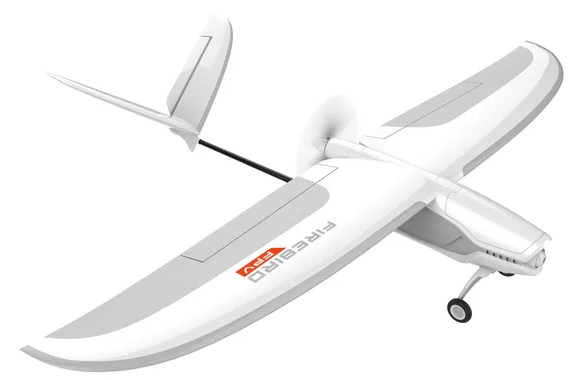
\includegraphics[width=\linewidth]{./img/png/uav-FirebirdFPV-FixedWing.png}
    \caption{Firebird: Fixed-wing~\cite{firebirdDrone}}
    \label{fig:uav-fixed-wing}
  \end{subfigure}\hfill
  \begin{subfigure}[t]{.32\textwidth}\centering
    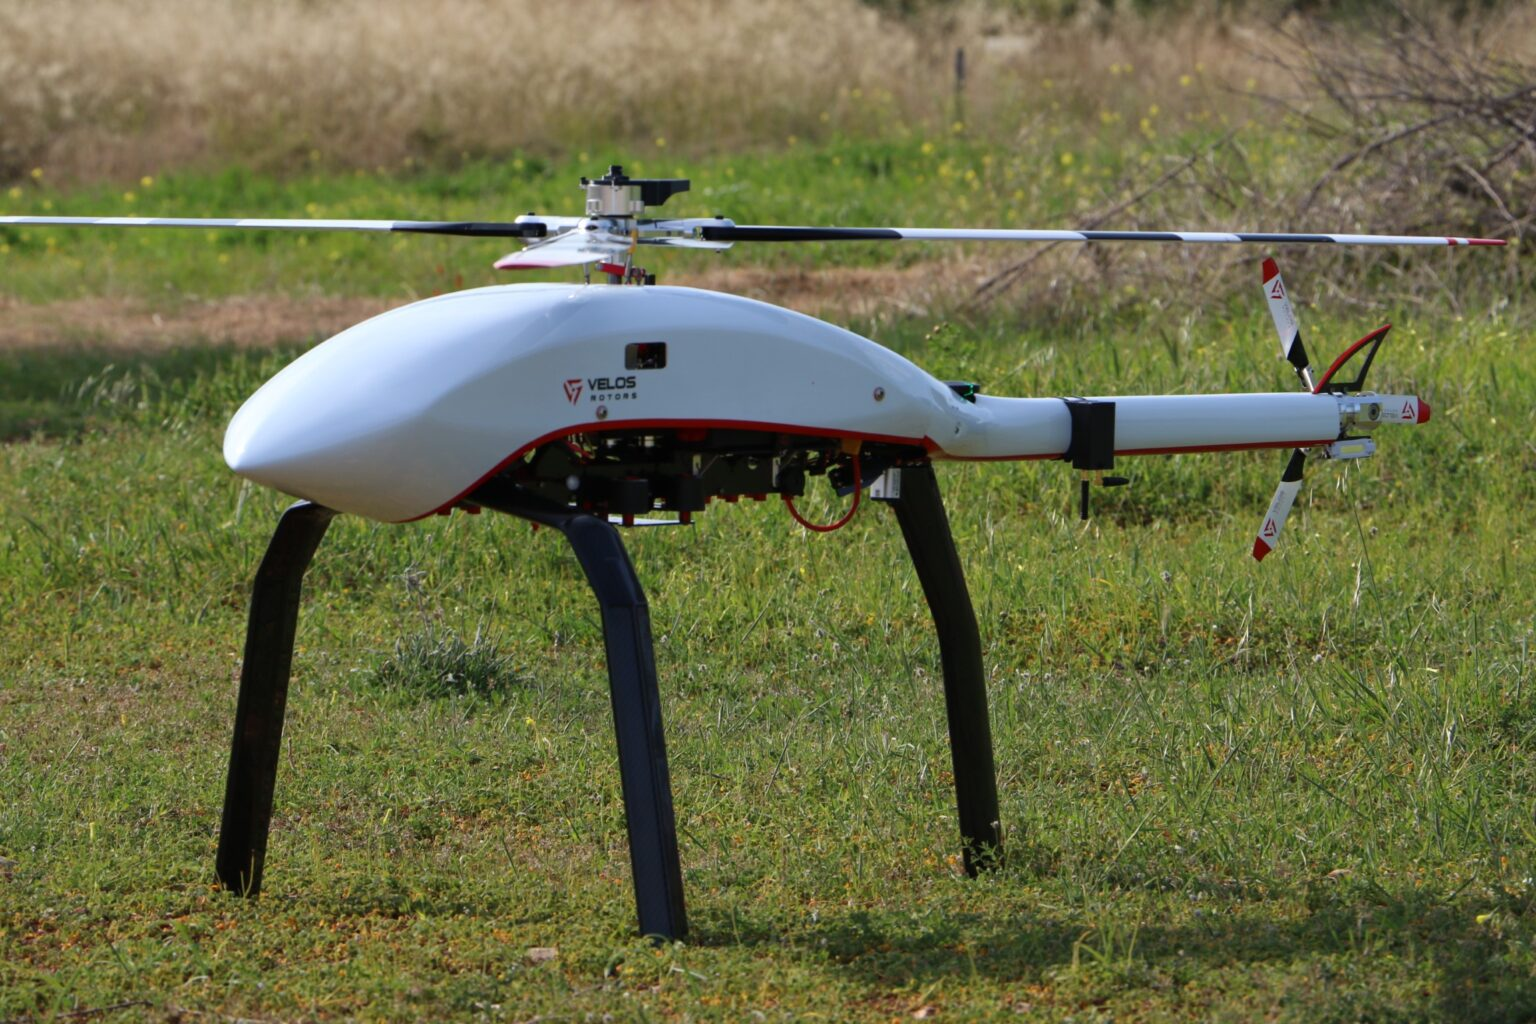
\includegraphics[width=\linewidth]{./img/jpg/uav-velos-singleRotor.jpg}
    \caption{Velos: single-rotor~\cite{velosDrone}}
    \label{fig:uav-single-rotor}
  \end{subfigure}\hfill
  \begin{subfigure}[t]{.32\textwidth}\centering
    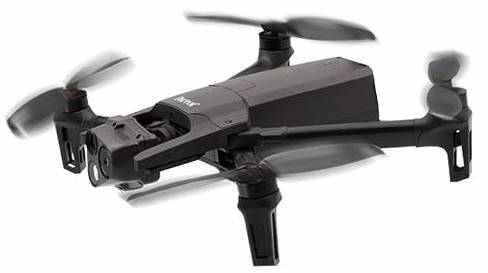
\includegraphics[width=\linewidth]{./img/jpg/uav-parrot-multirotor.jpg}
    \caption{Parrot: multirotor~\cite{parrotDrone}}
    \label{fig:uav-multirotor}
  \end{subfigure}

  \medskip % vertical space between rows

  %--------------------------- Row 2 ---------------------------%
  \begin{subfigure}[t]{.32\textwidth}\centering
    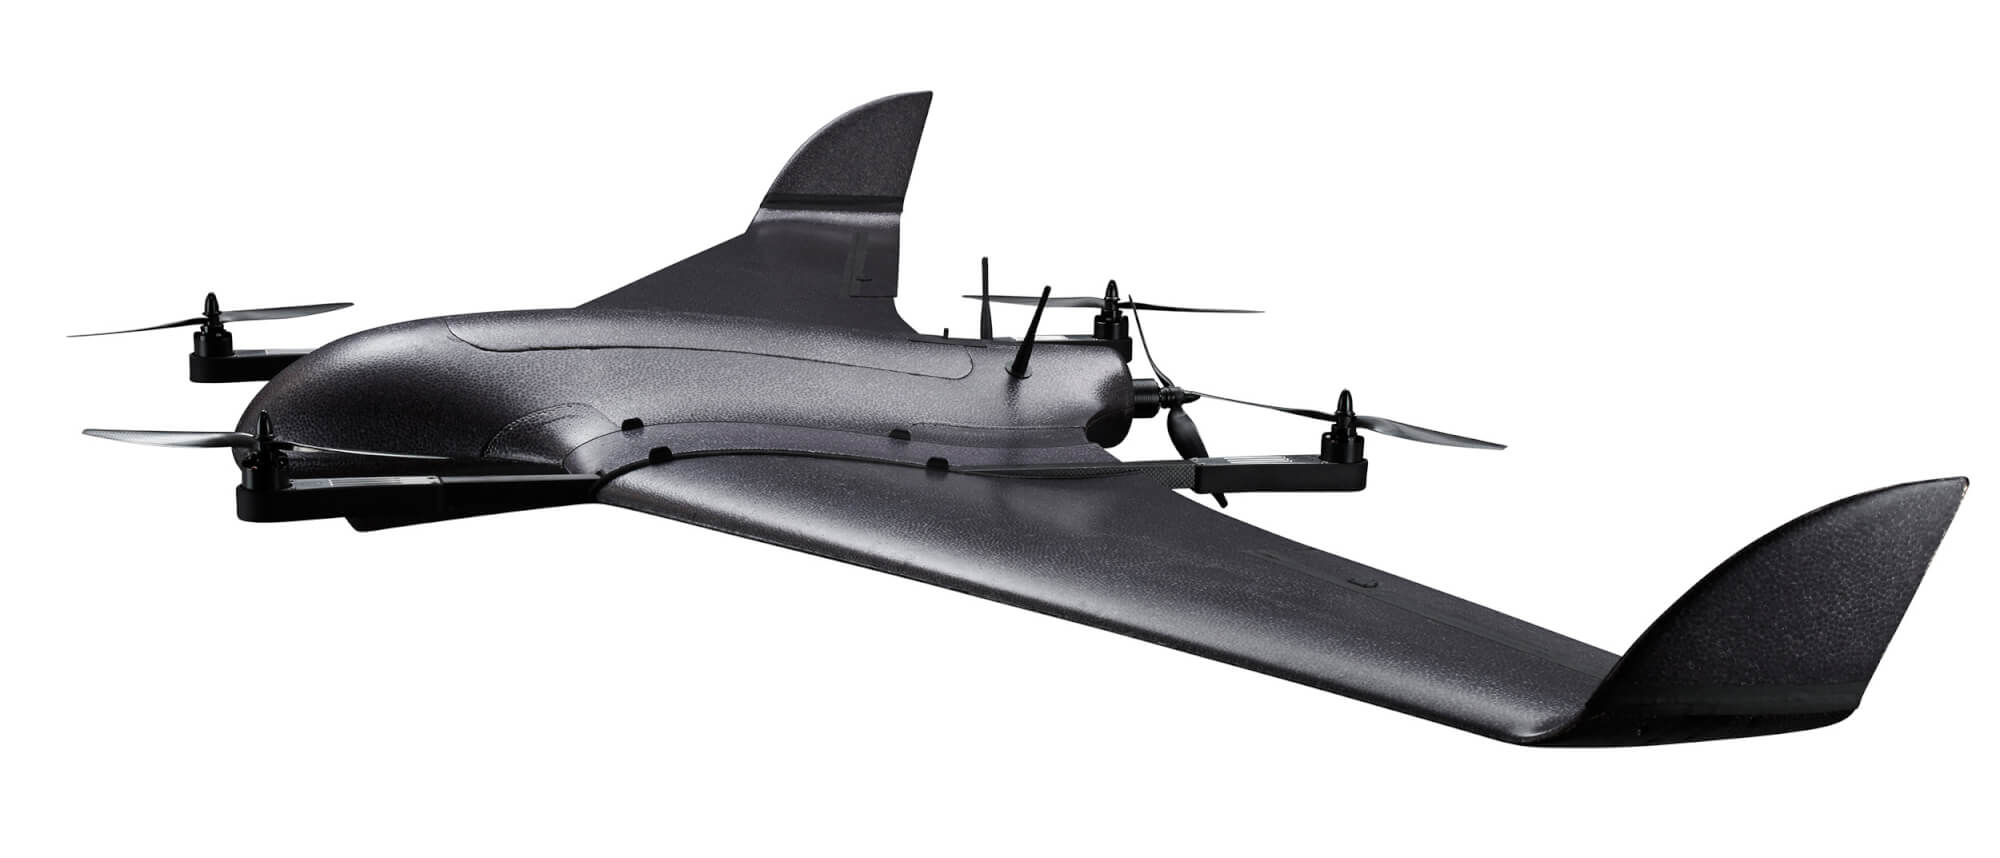
\includegraphics[width=\linewidth]{./img/jpg/uav-deltaQuadPro-hybrid.jpg}
    \caption{DeltaQuad Pro: fixed-wing hybrid~\cite{deltaQuadDrone}}
    \label{fig:uav-fixed-wing-hybrid}
  \end{subfigure}\hfill
  \begin{subfigure}[t]{.32\textwidth}\centering
    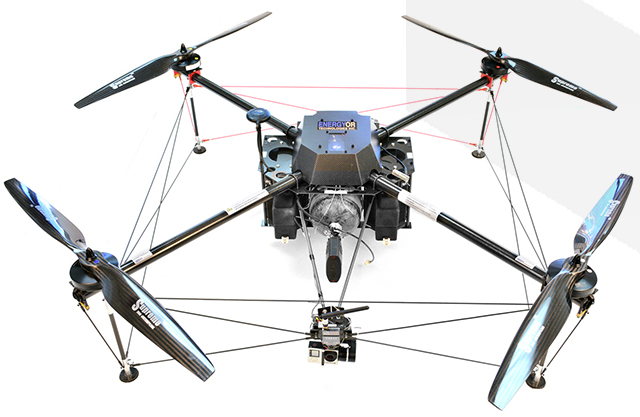
\includegraphics[width=\linewidth]{./img/jpg/uav-energyorQuad1000-hfc.jpg}
    \caption{Energyor Quad 1000: hybrid (HFC + batteries)~\cite{energyorDrone}}
    \label{fig:uav-energyor-hfc}
  \end{subfigure}\hfill
  \begin{subfigure}[t]{.32\textwidth}\centering
    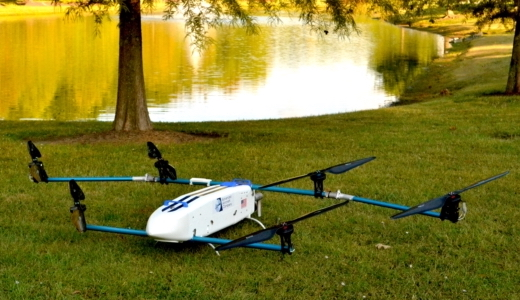
\includegraphics[width=\linewidth]{./img/jpg/uav-HAMR-FuelElectric.jpg}
    \caption{HAMR: hybrid (fuel+batteries)~\cite{hamrDrone}}
    \label{fig:uav-hamr-fuel}
  \end{subfigure}

  \medskip % vertical space between rows

  %--------------------------- Row 3 (centered single) ---------%
  % \makebox centers the single subfigure so the row is "3 x 3 x 1"
  \makebox[\textwidth][c]{%
    \begin{subfigure}[t]{.32\textwidth}\centering
      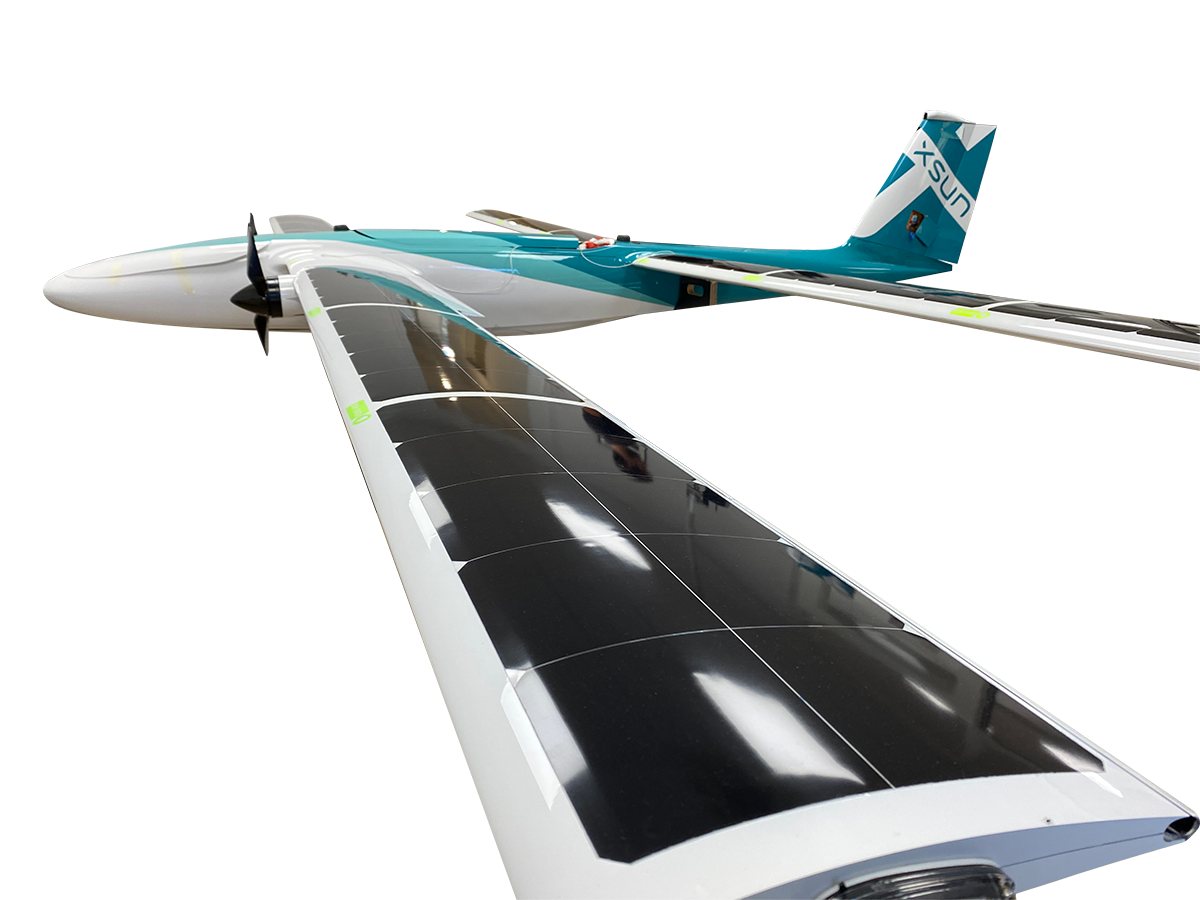
\includegraphics[width=\linewidth]{./img/png/uav-solarXOne.png}
      \caption{Solar X One: solar powered~\cite{solarXOneDrone}}
      \label{fig:uav-solarX}
    \end{subfigure}
  }

  \caption{UAV types examples}
  \label{fig:uav-types}
\end{figure}
%

The autonomy or endurance, refers to the maximum flight time with a
single charge (battery, fuel, or both), varying from a 20 or 30 minutes (small \glspl{uav}) to several
hours (large \glspl{uav}). Size, weight and weather conditions have a strong
impact on the autonomy. Some technologies are currently being developed to
support in-flight recharging through renewalable sources (\gls{pv} cells) or
wireless power techniques (e.g., laser emission)\cite{mohsan2022towards,mohsan_comprehensive_2022}.
Payload is the \gls{uav} lifting capacity,
varying from a few grams (small \glspl{uav}) to hundreds of kilograms (large
\glspl{uav}). Most common payloads are sensors and video
cameras~\cite{mohsan2022towards}.
Range is the maximum control distance and depends on the communication technology, network, and environmental conditions~\cite{mohsan2022towards}.
The altitude is the height a drone can fly, weather by
technological constraints or by legal ones~\cite{mohsan2022towards}.
%
Fig.~\ref{fig:uav-mindmap} depicts the \gls{uav}'s
generic overview, summarizing its main concepts.
%
%
\subsection{System overview}%
\label{sec:system-overview}
Fig.~\ref{fig:uav-sysOverv} shows an overview of the \gls{uav} system and its
ecosystem.
Positioned at the center of the figure (1) are the \gls{uav} and its associated flight control hardware and software.
Its main tasks are path planning, communication
management, data acquisition, and mission~\cite{aggarwal2020UAVPathPlanning}.

\begin{figure}[!hbt]
  \centering
  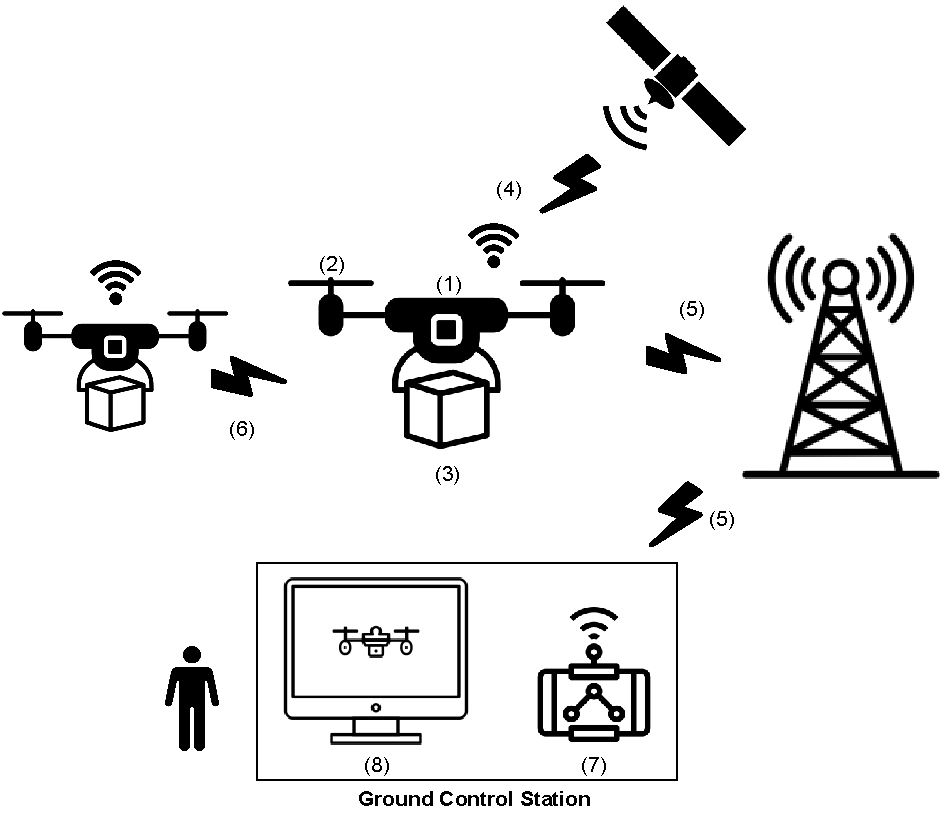
\includegraphics[width=0.7\textwidth]{./img/pdf/uav-sys-overv.pdf} 
%  \includesvg[width=1.0\textwidth]{./img/virtualization.svg} 
  %\caption[Virtualization mind map]{Virtualization mind map}%
  \caption[UAV system overview]{UAV system overview (adapted from~\cite{mohsan2022towards,aggarwal2020UAVPathPlanning})}%
  \label{fig:uav-sysOverv}
\end{figure}

The path planning works in
combination with the \gls{gcs} to assist in the navigation, finding the optimal
path, while providing environmental awareness through weather and climate
monitoring, and controlling the motion and speed for obstacle avoidance~\cite{aggarwal2020UAVPathPlanning}. To
achieve this, the
on-board flight controller collects data from multiple sensors
(e.g., \gls{imu}, barometer, \gls{gps} module, etc.) and,
together with the commands received from the \gls{gcs}, implements attitude
estimation and the control law (e.g., Kalman filter) to drive the propulsion
system (motors) (2)~\cite{px4-sysArch}.

The flight controller also manages three communication links~\cite{aggarwal2020UAVPathPlanning}: \gls{uav}\textendash\gls{gcs} (5), used for telemetry (e.g., audio/video) and human remote control (7, 8); \gls{uav}\textendash satellite (4), which provides weather, climate, and \gls{gps} data for accurate navigation~\cite{liang_toward_2024,alvarez-vanhard_uav_2021}; and \gls{uav}\textendash\gls{uav} (6), supporting cooperative missions and environmental awareness (e.g., danger signaling)~\cite{li_distributed_2024,azari_uav--uav_2020}.
%
The mission defines the flight objective, e.g., video capture or topographic
mapping~\cite{caroti_uav-borne_2017}, and directly determines the payload (3), such as a camera or \gls{lidar}~\cite{cai_branch_2024}.

Sensors can be typically grouped into obstacle-avoidance, payload, and
navigation~\cite{VogeltanzFreeSWUAVSurvey2016}. Ultrasonic and infrared sensors are generally used to avoid
collisions with obstacles, but \gls{tof} sensors like \gls{lidar} can also be
used, although more expensive and more complex.
Navigation relies on an \gls{imu} to estimate orientation and heading of the
vehicle, a barometer to used to estimate altitude with a precision of few
centimeters, and the \gls{gnss}/\gls{gps} module to estimate the
\gls{uav}'s geolocation for navigation and autonomous flight.
However, the geolocation has a precision of up to 5 meters, thus requiring
fusing the \gls{imu} and barometer data to improve accuracy~\cite{ebeidUAVPlatformsSurvey2017}.

Actuation depends on the propulsion system, but electronic drives are
ubiquitous. In a typical multirotor \gls{uav}, \glspl{bldc} motors drive the
rotors, controlled by an \gls{esc} -- a high-frequency inverter that converts
\gls{dc} supply to three-phase \gls{ac} and modulates motor speed~\cite{malyshev_research_2024}.
Fixed-wing hybrids additionally use servomotors for flaps~\cite{gabrielBLDCFixedWingUAV2011}.
%
Fig.~\ref{fig:uav-sysOverv-tasks-mindmap} depicts the concept map of \gls{uav}'s
tasks and components.
%

The \gls{uav} ecosystem can be outlined as a top-down view offive
layers~\cite{glossner2021overview} (Fig.~\ref{fig:uav-sysOverv-hierarc-mindmap}): (1) Flight
supervision, (2) Command and control, (3) System simulation, (4) operating
systems, and (5) physical hardware.
\emph{Flight supervision} covers flight management, safety/authorization, and remote
identification: commands flow from the \gls{gcs} to the \gls{fcs}; tools like
\lstinline{QGroundControl} provide path planning, mapping, and live telemetry;
fail-safes (e.g., geofencing, low-battery, loss of \gls{rc}/data link) must be
enforced by the pilot; airspace authorization can be obtained via services such
as \lstinline{LAANC} or \lstinline{Google Wing OpenSky}; and since 2023, remote
ID requires broadcasting a unique electronic identifier.
%
\emph{Command and Control} ensures safe flight via human-issued or
autopilot-generated commands over proprietary links or open \glspl{api} (e.g.,
MAVLink \gls{sdk}, Parrot \gls{sdk}).
Some notable open-source autopilots include \lstinline{PX4},
\lstinline{ArduPilot}, and \lstinline{Paparazzi UAS}.
%
\emph{System simulation} analyzes \gls{uav} behavior under varied conditions via
flight, traffic, and network-communication models. Simulators typically target a
specific domain~\cite{dimmig_survey_2025}: \gls{sitl}/\gls{hitl} environments
(e.g., Gazebo~\cite{garcia_simulation_2022} with PX4~\cite{px4-sim} and
ArduPilot-specific variants~\cite{arduPilot-sim}, or CoppeliaSim), and full
flight simulators such as FlightGear.
%
\emph{Operating systems} provide the hardware abstraction, ranging from
open-source \glspl{rtos} (\lstinline{NuttX}~\cite{px4-home},
\lstinline{ChibiOS}~\cite{arduPilot-home},
\lstinline{FreeRTOS}~\cite{librePilot-arch}) and \glspl{gpos}
(\lstinline{Linux}~\cite{px4-pilotpi}) to proprietary options
(\lstinline{VxWorks}~\cite{vxWorks-uav-aribus-helionic}). However, some
flight-control stacks run natively on the flight controller without a full
\gls{os} (e.g., \lstinline{Paparazzi UAS}~\cite{paparazzi-github},
\lstinline{iNAV}~\cite{inav-github}).
%
Finally, \emph{physical hardware} encompasses the
electronic platform, namely sensors, motors/actuators, and communication subsystems.


\subsection{Security and Safety}%
\label{sec:security-safety}
Another very important feature, often overlooked, is the \gls{uav}'s ecosystem
security, and alongside with it safety of people and goods~\cite{leccadito2018survey}. Security is often
not embedded in the system's design, posing all sorts of problems. For example,
\glspl{uav} often include onboard wireless communication modules that use open,
unencrypted, and unauthenticated channels, exposing them to a variety of
cyber-attacks~\cite{kishnaCyberVulnerUAVReview2017,mansfieldUAVCyberThreats2013}.
The problem is not restricted to
commercial applications, with the U.S. army banning Dji drones --- the most
widely used ones by the army --- for cybersecurity
concerns in 2017~\cite{suasNewsDjiDronesBanned2017}. Hacking of drones is
another major concern, exposing sensitive information and control of the
\gls{uav}. In fact, several incidents have been reported in the media where
drones were weaponized~\cite{spiegelUAVAccident2015,nytimesUAVAccident2018,theDriveUAVAccident2019}, and the volume and risk of such incidents are
likely to increase significantly with the expected drone market growth in the
foreseable future~\cite{mohsan2022towards} and the new regulations adopted by many countries which allow
drones to fly over populated areas~\cite{stocker2017UAVRegulationsReview}.

The most common attacks to the  \gls{uav} are \gls{dos} and \gls{ddos}, causing
resource availability challenges which can be exploited to drain the batteries,
overload the processing units, and flood the communications link, leading to
huge services' interruption~\cite{mohsan2022towards}. But more sophisticated attacks are used too, like
\gls{gps} spoofing -- impersonating as a valid \gls{gps} satellite to provide
false data, \gls{gps} jamming, instrument spoofing (gyroscope, compass), or even
killing the main process~\cite{nassi2021sok}. Ground control stations are a target too, since the
attacker can indirectly obtain access to the \gls{uav}, usually through key
loggers, viruses, and malwares,  and steal all of its data or send malicious
and erroneous commands to the \gls{uav}~\cite{mohsan2022towards}.

Nassi et al.~\cite{nassi2021sok} conducted a thorough and very extensive survey
on the security and privacy issues of \glspl{uav}, classifying attacks into
their target group: the \gls{uav} or people.
%
\emph{Attacks targeting
  \glspl{uav}} include compromises of onboard electronics (e.g., fake firmware,
instrument spoofing, \gls{gps} jamming), the airframe and payload (e.g., malicious \gls{cad} files, nets, bullets), the \gls{gcs} and the \gls{fpv} link
(deauthentication, video exfiltration, process killing, remote takeover), and
cloud backends used for telemetry storage.
%
Mitigations include authenticated or signed firmware, encrypted links with channel
hopping, real-time onboard monitoring and fault
containment~\cite{mohsan2022towards}, parachutes, and strong access controls
with two-factor authentication.
\emph{Attacks targeting people} span individuals, organizations, and states. The countermeasures follow a
detect-assess-interdict pipeline using radar, optical, infrared, \gls{lidar}, and
acoustic sensing, though none are foolproof (e.g., conventional radar has low
\gls{uav} reflectivity; acoustic signatures can be suppressed)~\cite{sathyamoorthy2015review}.
When a hostile \gls{uav} is
confirmed, interdiction options include nets, jammers, birds of prey, and
lasers, each with safety and effectiveness trade-offs~\cite{nassi2021sok}.

% Nassi et al.~\cite{nassi2021sok} conducted a thorough and very extensive survey
% on the security and privacy issues associated with \glspl{uav}, the attacks and countermeasures. The authors
% divided the security attacks on two categories:
% \begin{itemize}
% \item \textbf{Targetting \glspl{uav}}: corresponds to an attack an
%   ill-intentioned civilian performs on an \gls{uav} using, e.g., an \gls{sdr}, a
%   computer or a commercial laser. Six targets were identified --- the \gls{uav}
%   electronic hardware, the \gls{uav} chassis and package (e.g., propelers and
%   cargo), the \gls{gcs}, the \gls{fpv} channel, the pilot and cloud
%   services/servers. Attacks on the \gls{uav} hardware include installation of
%   fake firmware, instrument spoofing and \gls{gps} jamming. Countermeasures vary
%   with each attack, but, for example, the installation of fake firmware on the
%   device can be opposed by requiring the digital signature of the firmware
%   before installing. Direct attacks to interrupt \gls{uav}'s flight control and
%   commiunications links to modify mission parameters can be mitigated through
%   onboard software and hardware mechanisms, such as real-time monitoring,
%   instantaneous estimation of the controller, alert warning and immediate action
%   on any alteration from the intended controller model~\cite{mohsan2022towards}.
%   Attacks on the chassis and package include fake \gls{cad}
%   files to undermine its fabrication and deployment, especially critical for
%   open-source hardware, nets, and bullets. They can be opposed by requiring
%   digital signature and by using parachutes, respectively.
%   The \gls{fpv} channel is the radio communication channel between the \gls{uav}
%   and the \gls{gcs}, which enables the pilot to fly as if it was on board and
%   consists of a downlink --- used for video streaming --- and an uplink --- used
%   to control the \gls{uav} via the \gls{gcs}. The most known methods are
%   pilot's deauthentication, taking and dowloading videos and pictures, killing
%   the main process, or remote control of the drone, which can be mitigated
%   through the usage of an encrypted network protocol. Jamming is also an issue
%   and can be remediated using channel hopping. Lastly, cloud services and
%   servers expose the \gls{uav} indirectly to hackers, because, although most
%   \glspl{uav} are not connected to the Internet, the \gls{gcs} is, sending the
%   telemetry of flights to cloud servers for storage and analysis. The methods
%   used to explore this link are deanonymizing pilots and extracting flight
%   history, which can be both mitigated through the implementation of
%   authorization and two-factor authentication mechanisms.
% \item \textbf{Targetting people}: \glspl{uav} can attack people, on a
%   individual, organization or nation base. The countermeasures include
%   detection and tracking, assessment, and
%   interdiction. Several detection methods exist, such as radars,
%   video and infrared cameras, \gls{lidar}, acoustics, acoustics and optics,
%   etc. However, it is important to note that none of these methods are
%   fail-proof. For example, specific radars have to be used with very specialized
%   operators, since common radars are designed for large aircraft detection and
%   drones uses materials which are not very radio reflective. Another example is
%   the acoustics, where sensors exist to detect the specific spectrum of the
%   drone's propellers, but can be easily circumvented by going into silent
%   (stealth) mode~\cite{sathyamoorthy2015review}. Assessment concerns the rating
%   and identification of hostile drones, especially important in areas where
%   drones are used for both legal and illegal activies. The most used methods are
%   based on \gls{uav}'s classication, to identify the manufacturer and model of
%   the drone. In the event of the detection and assessment of a hostile drone,
%   interdiction must be applied, i.e., the drone should be disabled. For this
%   purpose, several methods can be used like bullets and nets, which are
%   dangerous and not very effective, commercial jammers, predator birds and laser
%   cannons.
% \end{itemize}

Safety failures pose risks to people and property and can be grouped into
several categories~\cite{ferrao2020stuart}. First, \emph{damage from calculation
errors} arises when the \gls{uav}'s flight is more dangerous than anticipated
(e.g., operating in restricted zones).
%
Second, \emph{sensor failures} occur because onboard sensors may fail to detect
delicate or transparent obstacles -- such as wires, tree branches, or glass --
leading to collisions, sometimes compounded by pilot overconfidence.
%
Third, \emph{obstacle deviation} can cause crashes into buildings or
vegetation due to sudden and unexpected changes in direction.
%
Fourth, \emph{direct attacks} use \glspl{uav} to harm individuals or steal
payloads (e.g., medical supplies), with recreational/hobbyist platforms being
frequent targets.
%
Finally, \emph{accidental damag}e results when a \gls{uav} goes out
of control due to operator error, cyber attack, or \gls{sw}/\gls{hw}
malfunction.
Regardless of the cause, a falling aircraft can inflict severe harm on people and goods.

Clearly, security and safety are fundamental aspects of the \gls{uav}'s
operation, but they require more effort to decrease the attack vectors and the
attack surface. Ferrão proposed that \gls{uav}'s design considers simultaneously
both aspects, as they strongly influence each
other~\cite{ferrao2020stuart}. Fig.~\ref{fig:uav-security-mindmap} illustrates the
\gls{uav}'s security and safety taxonomy.


% Safety failures are also very serious, since they pose risks on the integrity of
% people and goods. They can be categorized as follows~\cite{ferrao2020stuart}:
% \begin{itemize}
% \item \textbf{Damague due to calculation errors}: occurs when a \gls{uav} is
%   more dangerous than planned. For example, in 2020 in the U.K., an activist
%   group piloted hundreds of drones with the 3-mile depletion zone to interrupt
%   the flights, which could have been catastrophic.
% \item \textbf{Sensor failures}: \gls{uav} sensors do not easily detect delicate
%   objects, such as wires, tree branches, and transparent surface such as
%   buildings windows. Falls by collisions with these types of objects are very
%   common due to undetected obstacle or pilot's excess of confidence.
% \item \textbf{Obstacle deviation}: collisions and crashes caused by object
%   deviation are common, from building to trees.
% \item \textbf{Direct attacks}: these attacks are performed to harm people, for
%   personal or ideological reasons, or to steal the \gls{uav} payload, e.g., an
%   organ, food, or vaccines. The recreational/hobbyist \glspl{uav} are the most
%   commonly targets.
% \item \textbf{Accidental damage}: can occur when a \gls{uav} gets out of
%   control, due to legitimate loss of control by the owner, cyber attack, or
%   software or hardware malfunction. Indepently of the cause, the extent of the
%   damage on people as goods can be severe, due to crash of \gls{uav} falling
%   from the sky.
% \end{itemize}

\subsection{UAV Reference Hardware}%
\label{sec:uav-ref-hw}
In this section we discuss the reference hardware for \glspl{uav}.
Firstly, we present an overview over the hardware architecture. Then, we analyze
in more depth the open-source and commercial hardware solutions for \glspl{uav}.

\subsubsection{Overview and Architecture}%
\label{sec:overv-arch-hw}
Fig.~\ref{fig:uav-hw-arch} illustrates the high-level abstraction of the
\gls{uav} hardware architecture~\cite{leccadito2018survey,px4-sysArch}. The main
computing platforms are depicted in orange: (1) the flight controller or
\gls{fmu} (e.g., Pixhawk); (2) and, optionally,
the companion computer, which provides extra functionalities, off-loading the \gls{fcs}. More specifically, the companion computer can assist in the
navigation, preventing collisions and avoiding obstacles, support
mission-related tasks like camera surveillance or topographic mapping, and
process telemetry data.

\begin{figure}[!hbt]
  \centering
  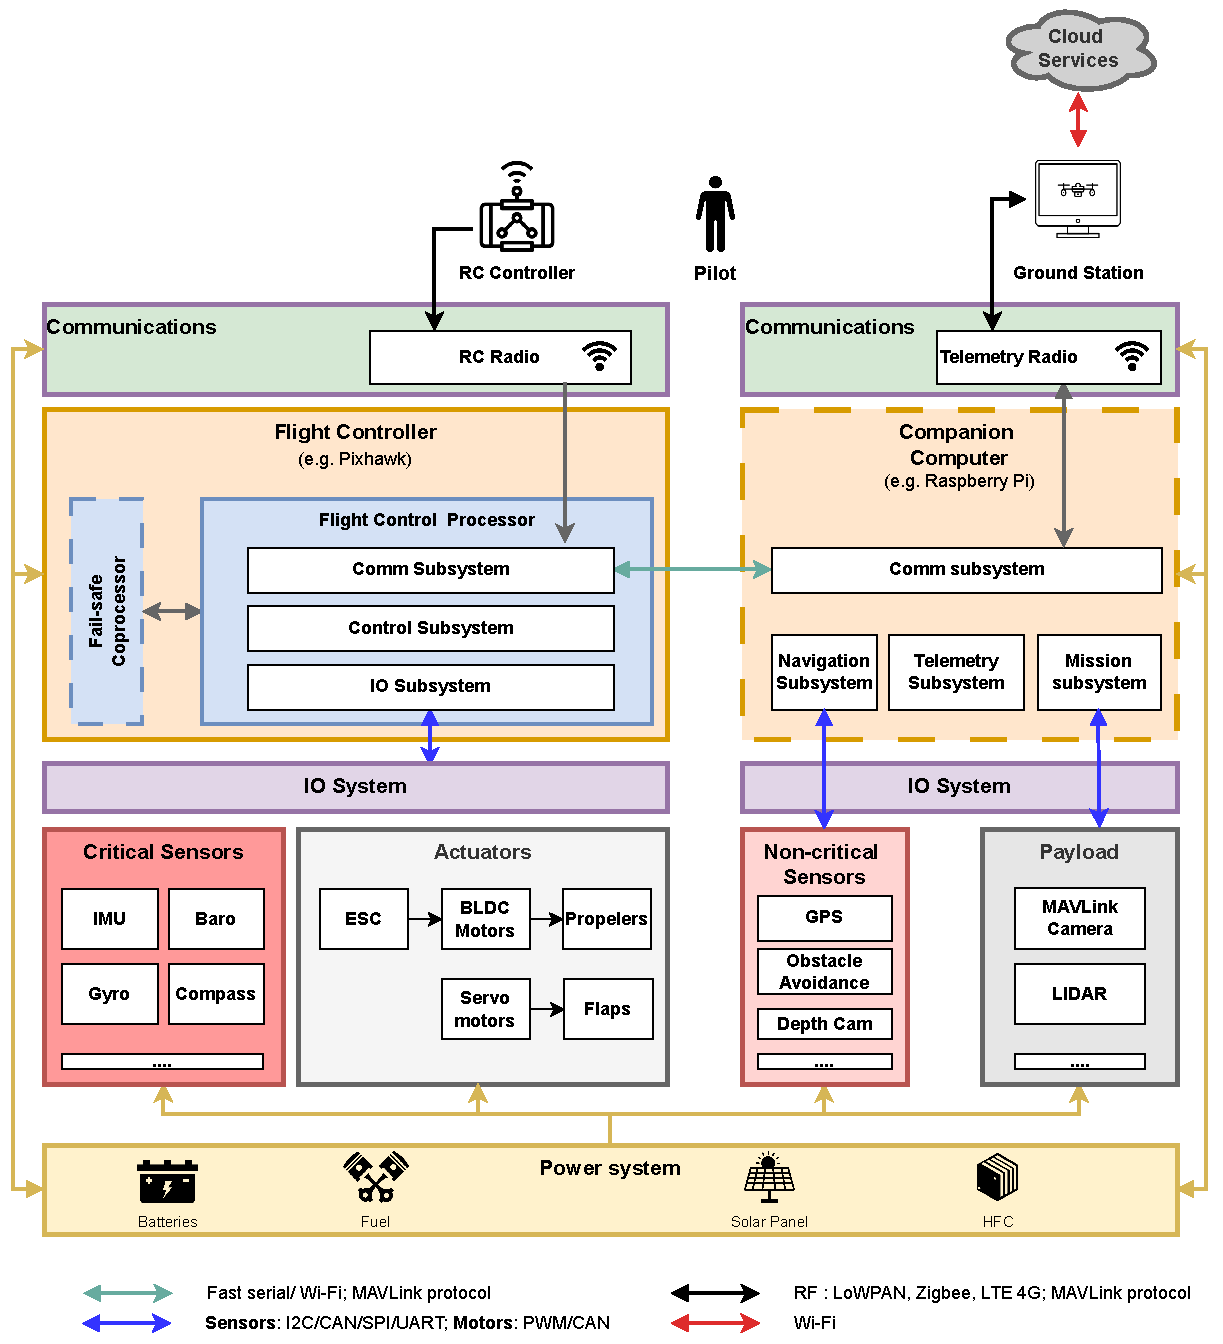
\includegraphics[width=1.0\textwidth]{./img/pdf/uav-hw-arch.pdf} 
  %\caption[Virtualization mind map]{Virtualization mind map}%
  \caption{UAV HW architecture: high-level abstraction}%
  \label{fig:uav-hw-arch}
\end{figure}

The \gls{fcs} is typically composed of a main processor, for \gls{uav} control,
and a optionally fail-safe coprocessor, dedicated to respond to failure events,
e.g., returning to base when the battery reaches the low threshold.
The main processor handles: (1) communications: processing commands arriving
from the manual \gls{rc} controller or between the companion computer; (2)
aircraft's control: typically using \gls{pid} models and/or estimation methods
(e.g., Kalman filter): (3) \gls{io}: to
interface the critical sensors, such as \gls{imu}, barometer, gyroscope, and
compass, or the actuators, such as \gls{bldc} motors and servomotors.
The power system supplies the required energy for computing and \gls{io}.

As aforementioned, the flight controller does not explicitly require the
companion computer, since the commands sent manually by the pilot
through the \gls{rc} controller are sufficient to navigate the aircraft
in \gls{los}. However, for autonomous missions, the non-critical
sensors such as the \gls{gps} and obstacle avoidance sensors are mandatory. In
this mode, the companion computer sends telemetry data to the \gls{gcs}, which
are typically superimposed on a map for straightforward navigation and receives
the navigational and mission-related commands, processing them and dispatching
the lower level commands to the flight controller or \gls{io} system.

\subsubsection{Open-source solutions}%
\label{sec:open-source-solut-hw}
\glsxtrfull{osh} solutions have been developed to provide more transparency,
extensibility, flexibility, maintainability, while trying to be
cost-effective. \gls{osh} means that the hardware design (i.e., mechanical
drawings, schematics, \gls{bom},\gls{pcb} layout data, \gls{hdl} source code),
and the software that drives the hardware, are all released under free/libre
terms~\cite{freeGNU}.
The user can purchase or manufacture the hardware components
individually or in \gls{cots} kits.

The \gls{osh} solutions fall into three main categories: Atmel-based,
ARM-based, and Companion Computer-based
platforms~\cite{ebeidUAVPlatformsSurvey2017}. The first two target the
\gls{fmu}, while the last provides a \gls{fmu} + companion-computer solution in
one package. Until recently, the Atmel-based platforms, such as the ArduPilot
Mega (APM), were still being produced. This product featured the 8-bit ATmega 2560 \gls{mcu}, which includes an \gls{imu} and, optionally, a
compass and a \gls{gps}~\cite{ardupilotMega}. Its biggest advantage is that it could be programmed using the
Arduino \gls{ide}, enabling easy customization of the ArduPilot firmware's
features by hobbyists. The complexity level of modern autopilots require more
powerful \gls{mcu}, dictating the deprecation of the 8-bit
ones~\cite{fmu8BitDeprecation}.

Currently, the vast majority of \gls{osh} projects are based on 32-bit ARM platforms
(\lstinline{Pixhawk 4}, \lstinline{CC3D}, \lstinline{Paparazzi Chimera},
\lstinline{CUAV v5 Plus}, etc.) and supported by initiatives
like the Pixhawk hardware standardization. Pixhawk is a company that develops open
standards for drone hardware, providing readily available hardware
mechanical and electrical specifications and guidelines for drone development~\cite{pixhawk}.
%
The \lstinline{Pixhawk 4} (see Fig.~\ref{fig:osh-pixhawk4}) is a flight
controller developed in collaboration by the Holybro manufacturer and the PX4
software teams, and suitable for academic and commercial developers~\cite{pixhawk4}.
It was released under the \gls{bsd} license, comprising two 32-bit ARM
processors: an Cortex-M7 STM32F765 as the main \gls{fmu} processor and a
Cortex-M3 STM32F100 as an \gls{io} coprocessor. The Pixhawk 4 comes with
on-board sensors (accelerometers/gyroscopes, magnetometer, and barometer) and a
\gls{gps} module, and supports the \gls{pwm}, \gls{can} \gls{i2c}, \gls{uart},
\gls{spi}, for sensors and actuators operation. The \gls{uart} and telemetry
interfaces are also available for communication with an off-board
computer~\cite{pixhawk4} and remote controller. The Pixhawk 4 runs the PX4
autopilot on top of the NuttX \gls{rtos}.
%
The \lstinline{CUAV v5 Plus} is another flight controller that uses the dual Arm
Cortex-M7 architecture for \gls{fmu} and \gls{io}~\cite{arduPilot-cuavV5}. It
was released under the \gls{bsd} license and runs the ArduPilot
firmware. On the other hand, the \lstinline{Paparazzi Chimera} is an \gls{osh}
flight controller that integrates all \gls{io} in the same same board, based on
a ARM Cortex-M7 STM32F767 \gls{mcu}~\cite{paparazziChimera}. It was released
under the \gls{gpl} license and runs the Paparazzi
autopilot~\cite{paparazzi-github}. All the ARM-based platforms feature small
on-board memory, typically up to 2 MB of Flash memory and 512 KB of \gls{sram} memory.
  
% Pixhawk 4
\begin{figure}[!hbt]
  \centering
  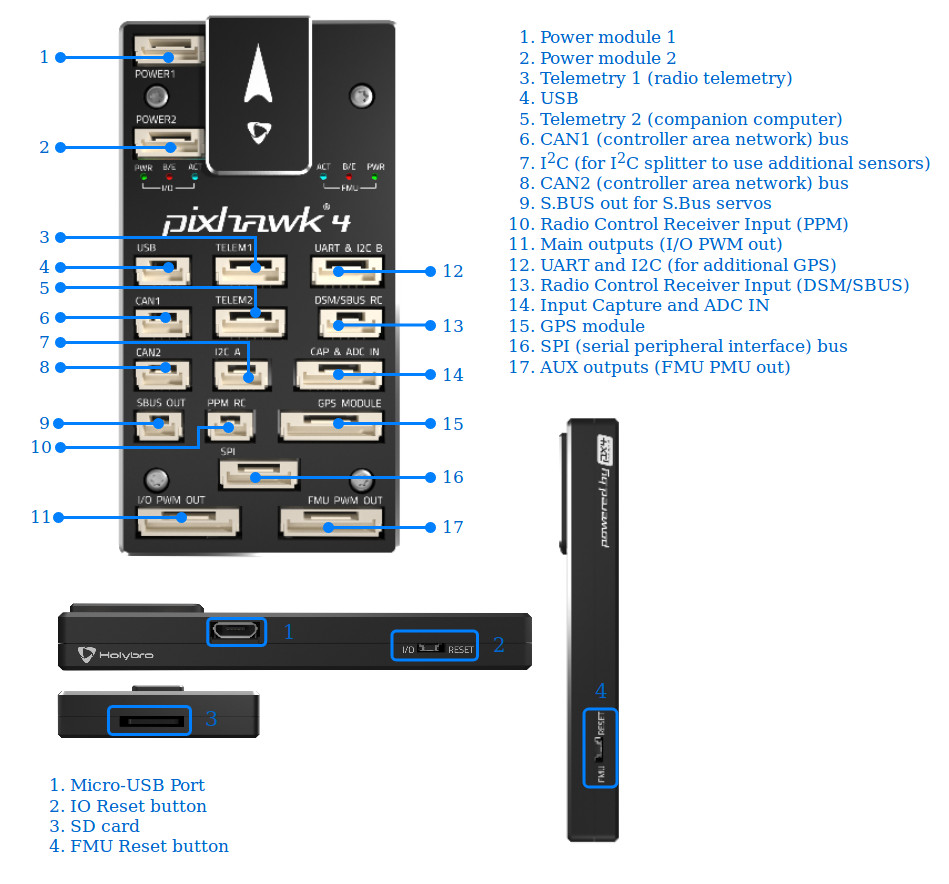
\includegraphics[width=0.7\textwidth]{./img/jpg/osh-pixhawk4.jpg} 
  \caption[Pixhawk4 flight controller]{Pixhawk 4 flight controller~\cite{pixhawk4}\footnotemark}%
  \label{fig:osh-pixhawk4}
\end{figure}
\fnlicCCFour{foot:cc-lic-pix}% CC licence

The companion computer-based platforms expands \gls{io} functionality through a daughter
board, like the Erle-Brain 3 or PXFmini~\cite{ebeidUAVPlatformsSurvey2017}, while using the Arm Cortex-A to run a
custom Linux \gls{gpos} with a preemptive kernel option that hosts the flight
control stack~\cite{erle-brain}. The PXFMini, for example, weighs only fifteen
grams and was assembled on top of a single-core Raspberry Pi Zero, providing
on-board barometer and \gls{imu} sensors, expansion ports, and a triple
redundant power supply~\cite{pxfmini}. Unfortunately, the Erle-Brain 3 and PXFmini were
deprecated after the Erle Robotics company was bought out~\cite{pxfmini-deprec}.

The PilotPi shield is a Raspberry~Pi–based platform targeted at hobbyists. It
offers a fully open-source solution for running the PX4 autopilot directly on
Raspberry~Pi, requiring no proprietary drivers and providing open-source
\gls{pcb} designs and schematics~\cite{px4-pilotpi}. Fig.~\ref{fig:pilotpi}
shows the shield stacked on a Raspberry~Pi~4. The intermediate board integrates
the typical \gls{uav} sensors (\gls{imu}, compass, barometer) and exposes
\gls{gps} and telemetry radio as \gls{uart} devices. The top board handles power
distribution and management, motor actuation, and additional peripherals
accessible via the \gls{gpio} header.

% Pixhawk 4
\begin{figure}[!hbt]
  \centering
  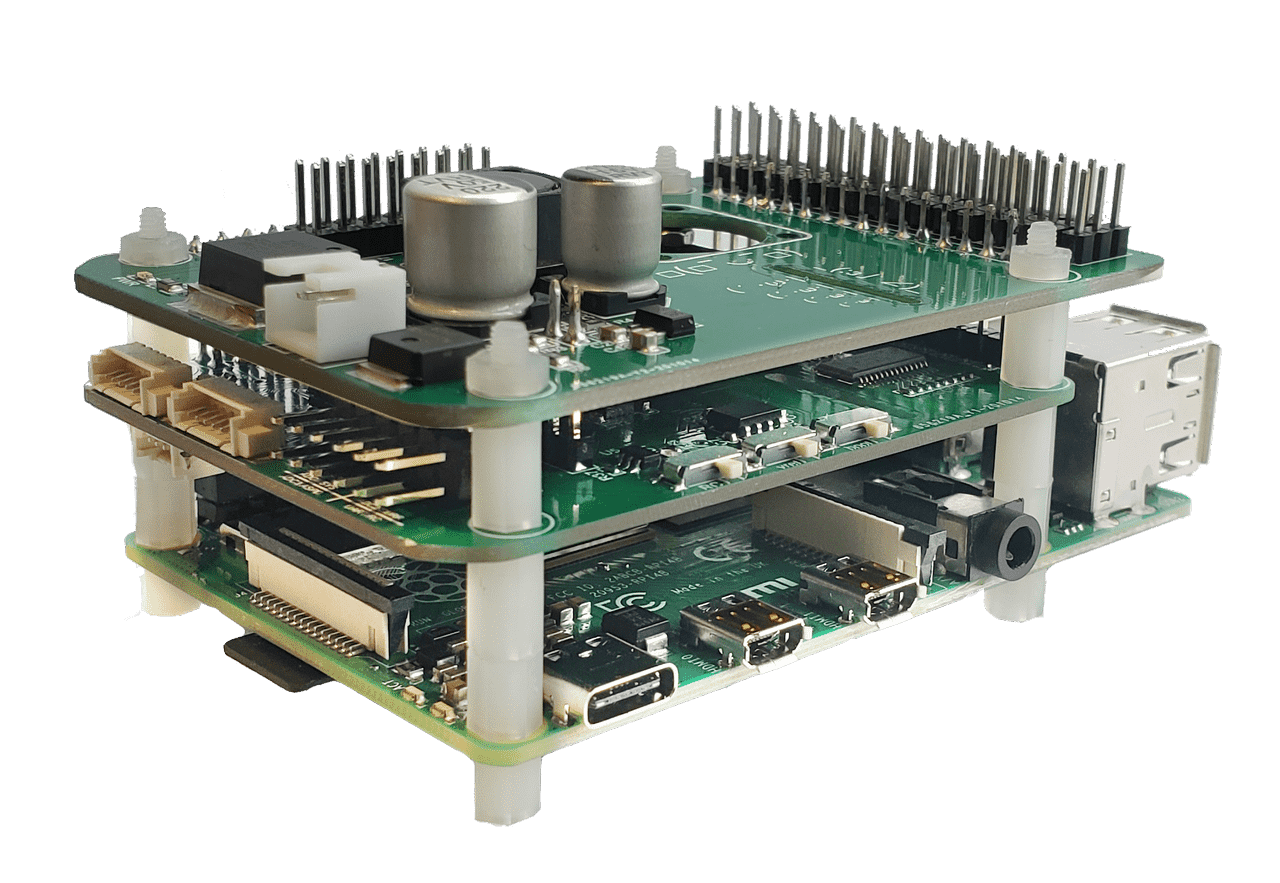
\includegraphics[width=0.7\textwidth]{./img/png/rpi-pilotpi} 
  \caption[PilotPi shield]{PilotPi shield~\cite{px4-pilotpi}\footnotemark}%
  \label{fig:pilotpi}
\end{figure}
\fnlicCCFour{foot:cc-lic-pilotpi}% CC licence

  % This flight controller integrates all \gls{io} in the same board, and it uses the  @ 216 MHz (2 MB Flash,
  % 512 Kb \gls{sram}) \gls{mcu}. It comes with on-board sensors
  % (\gls{imu}, barometer, and pressure sensure), an XBEE modem holder for
  % communications, and a dedicated serial link and power supply for the companion
  % computer (e.g., Beaglebone, RaspberryPi, etc.).

%   It has \gls{pwm}, \gls{can}
%   \gls{i2c}, \gls{uart}, \gls{spi}, and servomotors interfaces~\cite{pixhawk4}.
  
% % Paparazzi Chimera
% \begin{figure}[!hbt]
%   \centering
%   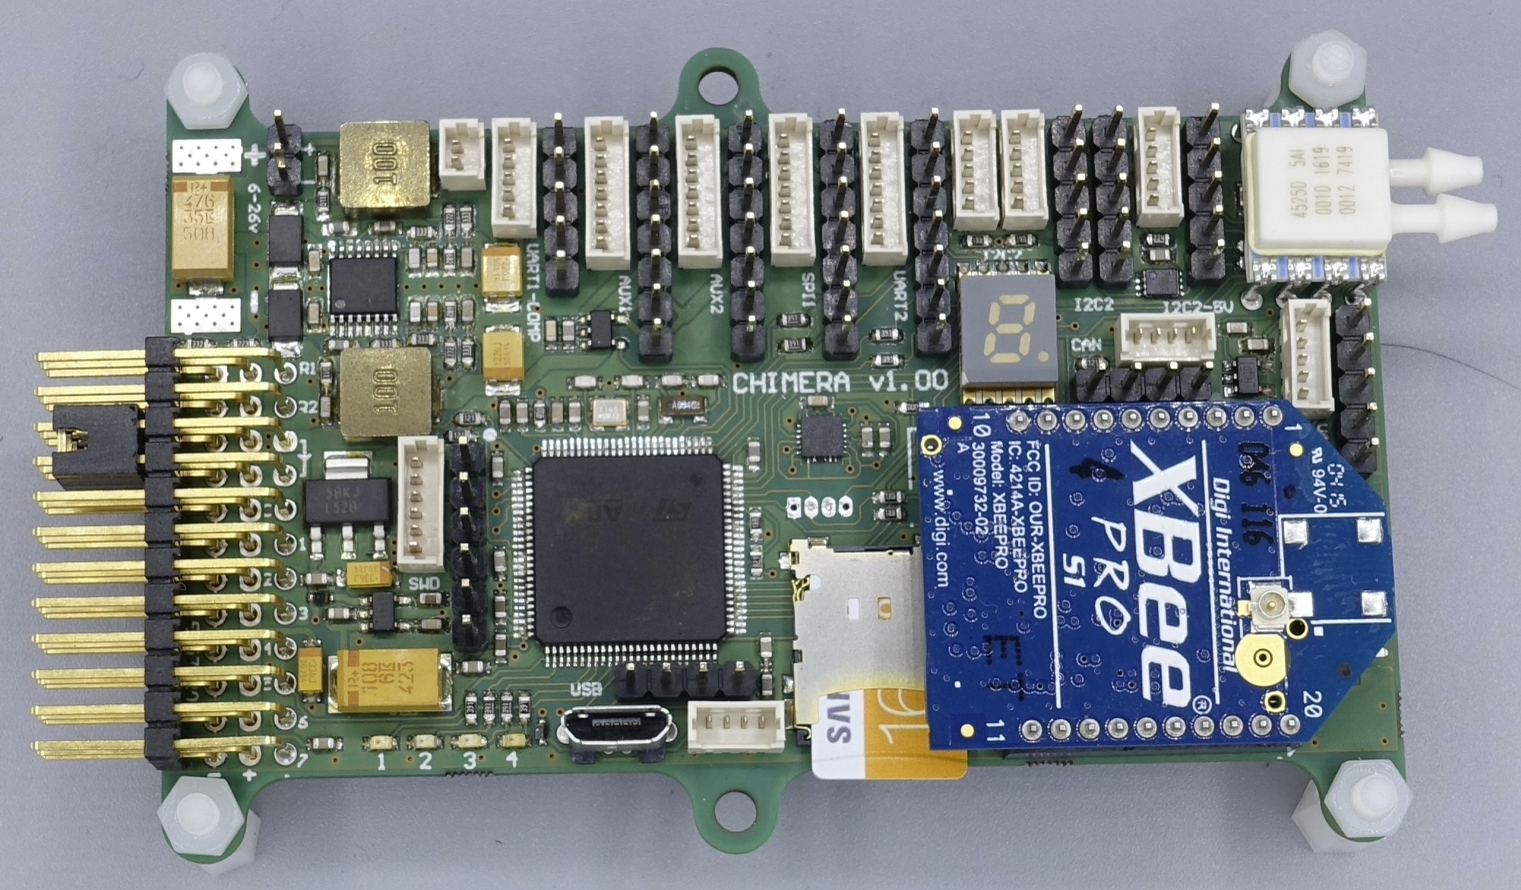
\includegraphics[width=0.6\textwidth]{./img/png/osh-paparazzi-chimera.png} 
%   \caption{Paparazzi Chimera flight controller~\cite{paparazziChimera}}%
%   \label{fig:osh-paparazzi-chimera}
% \end{figure}
  
%   The \lstinline{CC3D} is an \gls{osh} flight controller released
%   under the \gls{gpl} license~\cite{cc3d} (see
%   Fig.~\ref{fig:osh-cc3d}), running the \lstinline{OpenPilot} firmware. It uses a STM 32-bit \gls{mcu} @ 90
%   MHz (128 kB Flash and 20 kB \gls{sram}). It comes with on-board gyroscope and
%   accelerometers, support to serial and \gls{usb} telemetry, up to ten motors,
%   and provides camera stabilization.
  
% % CC3D
% \begin{figure}[htb!]
%   \centering
%   %
%   \begin{subfigure}[t]{0.8\textwidth}
%   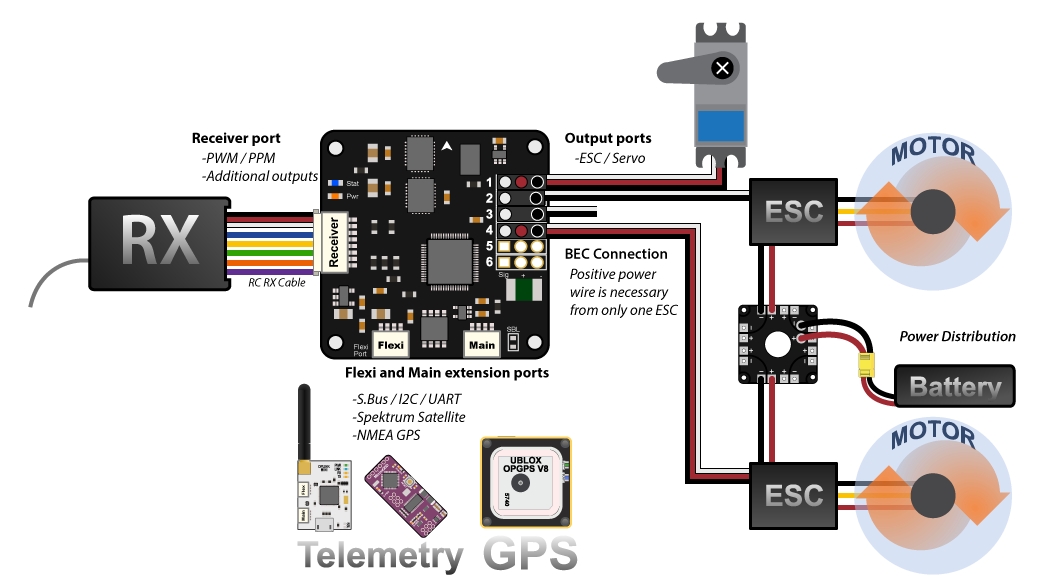
\includegraphics[width=1.0\textwidth]{./img/png/osh-cc3d-conn.png}
%   \caption{Connection diagram}%
%   \label{fig:osh-cc3d-conn}
%   \end{subfigure}
% %
%   \begin{subfigure}[t]{0.35\textwidth}
%   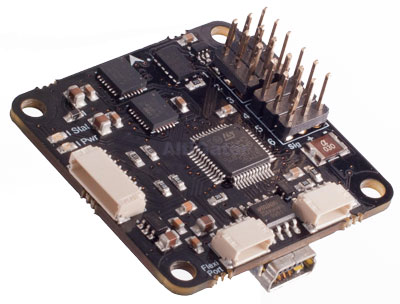
\includegraphics[width=1.0\textwidth]{./img/png/osh-cc3d-board.png}
%   \caption{flight controller board}%
%   \label{fig:osh-cc3d-board}
% \end{subfigure}
% %
%   \caption{CC3D flight controller~\cite{cc3d}}%
%   \label{fig:osh-cc3d}
% \end{figure}
% %
  
% CUAV V5 Plus
% \begin{figure}[!hbt]
%   \centering
%   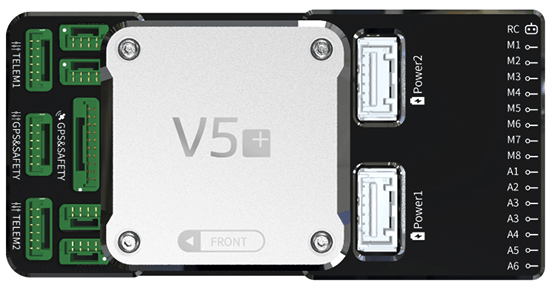
\includegraphics[width=0.6\textwidth]{./img/png/osh-cuav-v5.png} 
%   \caption{CUAV v5 Plus flight controller~\cite{arduPilot-cuavV5}}%
%   \label{fig:osh-cuav-v5}
% \end{figure}

\subsubsection{Commercial solutions}%
\label{sec:commercial-solutions-hw}
The commercial solutions are generally proprietary in nature, and thus closed-source. The
lack of transparency can be an issue, raising suspicions, like the on-going ban
of the U.S. Army to the Dji
drones~\cite{suasNewsDjiDronesBanned2017,djiBan2022}. Nonetheless, proprietary
solutions represent 70\% of the market share, with Dji being the biggest
manufacturer~\cite{droneAnalyst2021}.
%
The commercial solutions can be classified into three main categories: microcontroller-based, \gls{fpga}-based, and Companion Computer-based
platforms.
Historically, it is important to mention the deprecated 8-bit Atmel platforms,
such as the HobbyKing KK.2.1.5. This product featured an Atmel Mega644PA
8-bit AVR with 64 KB of memory, a MPU-6050 \gls{imu} sensor, and a \gls{lcd} and
push buttons for user interaction~\cite{hobbykingKK2}. It came pre-installed
with the KK2 firmware, but it could also run the ArduPilot software
stack.
%
The \lstinline{SPRacing H7 Extreme} is a low-end flight controller featuring the
Arm STM32H750 \gls{mcu}~\cite{spRacing}
with an external 128 MB flash
memory and all the common onboard sensors and interfaces. Targeted at the \gls{uav} racing market, it supports \gls{fpv} video
streaming through the available camera interfaces~\cite{spRacing}. It commonly
runs \lstinline{Betaflight} or \lstinline{Cleanflight}, though it is also
compatible with
\lstinline{ArduPilot}~\cite{arduPilot-SPRacing}.% \paragraph{Microcontroller-based
% platforms}
%  
% SPRacing H7 extreme
% \begin{figure}[htb!]
%   \centering
%   %
%   \begin{subfigure}[t]{0.25\textwidth}
%   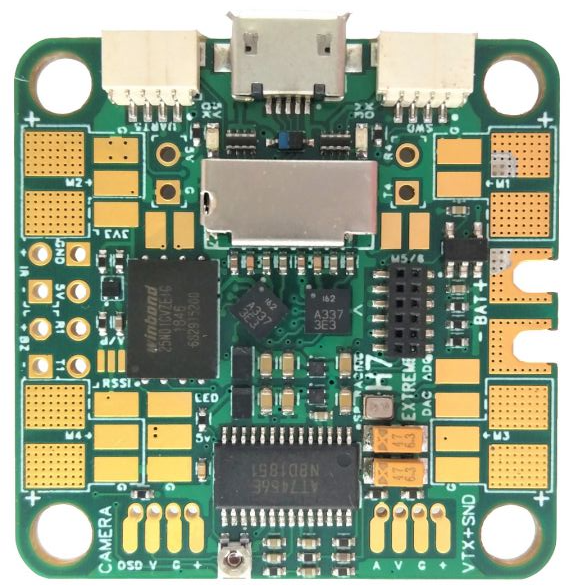
\includegraphics[width=1.0\textwidth]{./img/png/hw-SPracing-H7-extreme.png} 
% %  \caption{Connection diagram}%
% %  \label{fig:osh-cc3d-conn}
%   \end{subfigure}
% %
%   \begin{subfigure}[t]{0.25\textwidth}
%   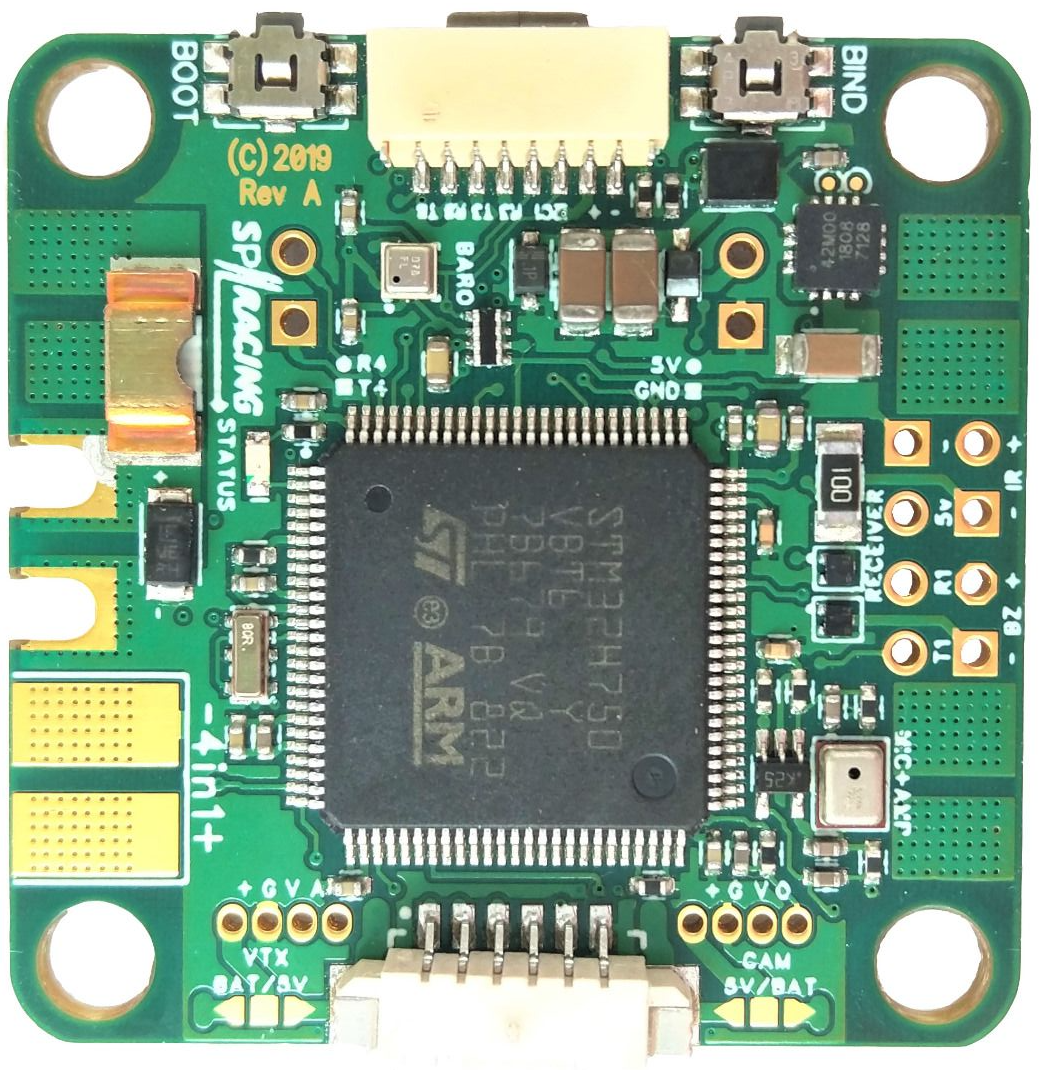
\includegraphics[width=1.0\textwidth]{./img/png/hw-SPracing-H7-extreme2.png} 
%  % \caption{flight controller board}%
%  % \label{fig:osh-cc3d-board}
% \end{subfigure}
% %
%   \caption{SPRacing H7 extreme flight controller~\cite{arduPilot-SPRacing}}%
%   \label{fig:hw-SPRacing}
% \end{figure}
%

% \paragraph{FPGA-based platforms}
The \lstinline{Aerotenna OcPoC-Zynq Mini} is a \gls{fpga} + ARM \gls{soc} based
  flight control platform,  which supports the ArduPilot and PX4 software
  stacks~\cite{ocpoc} (see Fig.~\ref{fig:hw-ocpoc}). Released back in 2017, it
  is currently discontinued~\cite{ocpoc-discontinued}.
  The Artix-7 \gls{fpga}, with 28 thousand logic cells, provided \gls{ai}
  capabilities and \gls{io}'s flexibility, crucial for rapid sensor integration
  and customization of the flight controller hardware. The ARM Cortex-A9
  dual-core runs Linux to support the autopilot and for data logging and
  processing, and includes 512 MB \gls{ram} and 128 MB of flash memory. The OcPoc-Zynq Mini supported
  triple-redundancy in the \gls{gps}, magnetometers, and \glspl{imu} on top of
  the conventional on-board sensors, programmable in the
  \gls{fpga}~\cite{ocpoc}.

% Ocpoc
\begin{figure}[!hbt]
  \centering
  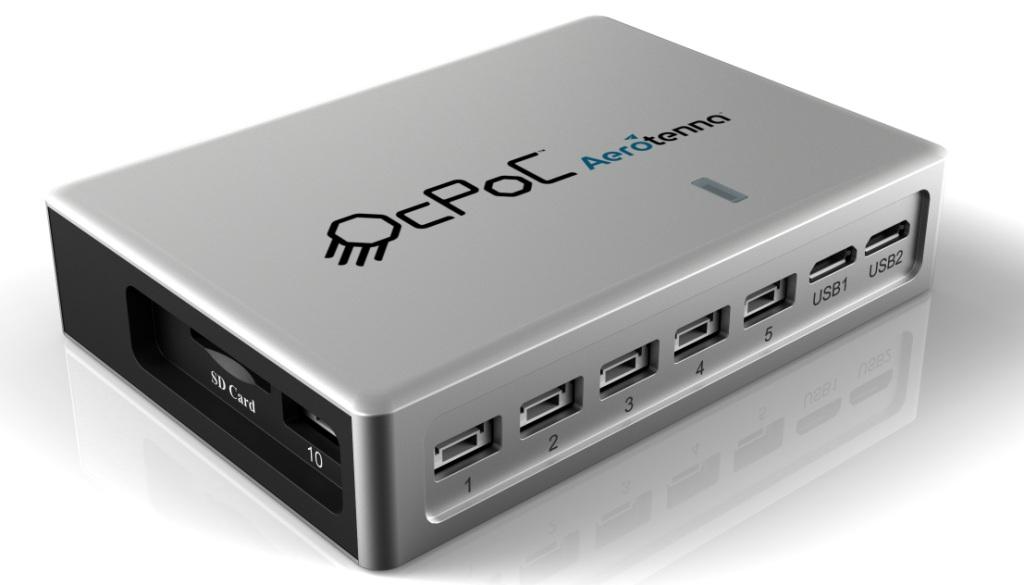
\includegraphics[width=0.5\textwidth]{./img/png/hw-ocpoc-zynq-mini.png} 
  \caption[Aerotenna OcPoc-Zynq Mini flight controller]{Aerotenna OcPoc-Zynq Mini flight controller~\cite{ocpoc}\footnotemark}%
  \label{fig:hw-ocpoc}
\end{figure}
%
\fnlicCCFour{foot:ocpoc}%

%\paragraph{Companion Computer-based platforms}
The most notable companion computer-based platforms are the Navio2,
the PixC4-Jetson, and the Auterion Skynode X/S.  
Similarly to PilotPi, the \lstinline{Navio2} flight controller consists of a
Raspberry Pi shield, but the hardware design is closed-source.
Navio2 runs a custom version of the Raspberry Pi OS (debian-based)~\cite{navio2-sw}, which supports ArduPilot and PX4 software
stacks~\cite{arduPilot-Navio2,navio2-px4}.
  The shield includes on-board
  sensors (dual \gls{imu}, barometer), a \gls{gnss} receiver, an \gls{rc}
  \gls{io} coprocessor, \gls{i2c}, and
  \gls{uart} interfaces for sensors and radios, 14 \gls{pwm} servomotors
  outputs, and a triple redundant power supply~\cite{arduPilot-Navio2}.

% NAVIO2
% \begin{figure}[!hbt]
%   \centering
%   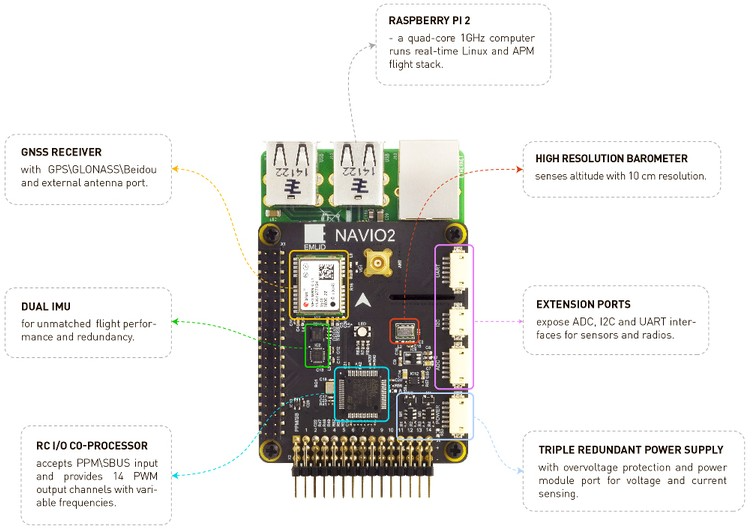
\includegraphics[width=1.0\textwidth]{./img/png/osh-NAVIO2} 
%   \caption{NAVIO2 flight controller~\cite{arduPilot-Navio2}}%
%   \label{fig:osh-NAVIO2}
% \end{figure}

  The \lstinline{PixC4-Jetson} (Fig.~\ref{fig:hw-horizonJetson}) is a
  professional high-end flight controller that integrates an dual-ARM
  \gls{fmu} and \gls{io} processors, and the Nvidia Jetson companion
  computer~\cite{arduPilot-horizonJetson}. This flight controller supports the
  ArduPilot and PX4 software stacks and can be remotely configured through a
  remote terminal~\cite{arduPilot-horizonJetson}. Thus, extra security measures are required, with the
  PixC4-Jetson providing a \gls{lte} connection management with a Layer-2 peer
  to peer \gls{vpn} and a secure cloud connection to Horizon31's
  U.S. servers~\cite{arduPilot-horizonJetson}. The live video streaming is
  assured by multiple-endpoint encoding pipelines and optional access to
  Horizon's cloud low-latency web\gls{rtc} video distribution system.
  %
  The Nvidia Jetson companion computer is well-suited fo computer vision,
  machine learning, and \gls{ai} tasks, further enhancing the capabilities of
  the \gls{uav}~\cite{jetson-docs}.

% Horizon Jetson
\begin{figure}[htb!]
  \centering
  %
  \begin{subfigure}[t]{0.9\textwidth}
  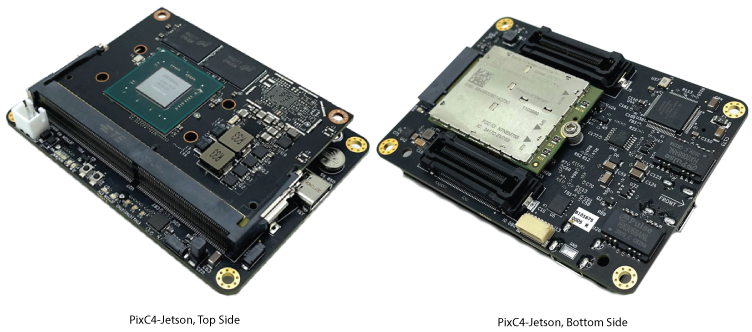
\includegraphics[width=1.0\textwidth]{./img/png/hw-horizon-pixc4-jetson.png} 
  \caption{Board}%
  \label{fig:hw-horizonJetson-board}
  \end{subfigure}
%
  \begin{subfigure}[t]{0.9\textwidth}
  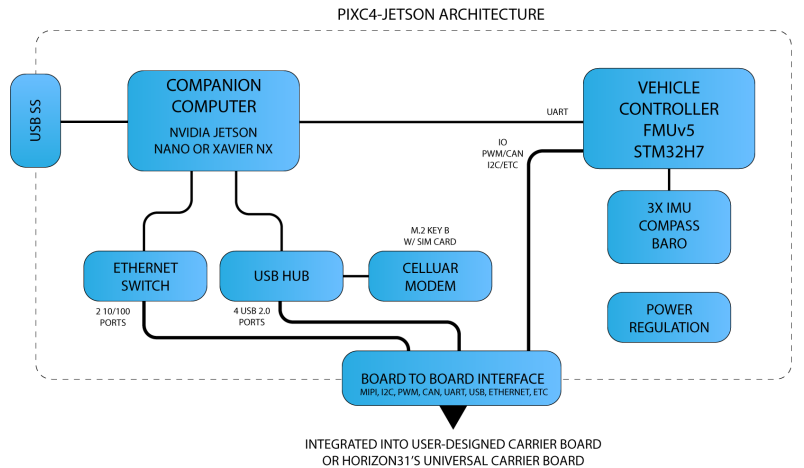
\includegraphics[width=1.0\textwidth]{./img/png/hw-horizon-pixc4-jetson-arch.png} 
  \caption{HW architecture}%
  \label{fig:hw-horizonJetson-arch}
\end{subfigure}
%
  \caption[Horizon31 PixC4-Jetson flight controller]{Horizon31 PixC4-Jetson flight controller~\cite{arduPilot-horizonJetson}\footnotemark}%
  \label{fig:hw-horizonJetson}
\end{figure}
%
\fnlicCCFour{foot:jetson-hw-sw}%

% Skynode X
Another relevant option in the commercial market is the \lstinline{Auterion Skynode X},
combining a flight controller, a mission computer and \gls{lte} connectivity all
in on product~\cite{skynodeXWebsite} in a compact form factor.
%
The \gls{fmu}, based on the Pixhawk FMUv6 architecture, comprises the 
a STM32H753 microcontroller and the STM32F103 \gls{io} coprocessor, and a
triple-redundant inertial sensor to minimize failure risk~\cite{skynodeXDatasheet}.
It supports up to 8 \gls{uart}, a dual redundant \gls{can},
100Base-TX Ethernet, 16 \gls{pwm} outputs, 2 \gls{i2c} and 1 \gls{spi}
connections. The \gls{fmu} runs an enterprise-hardened version of PX4, labelled
as Auterion PX4 (APX4)\cite{skynodeXDatasheet}.
%
% \begin{figure}[!hbt]
%   \centering
%   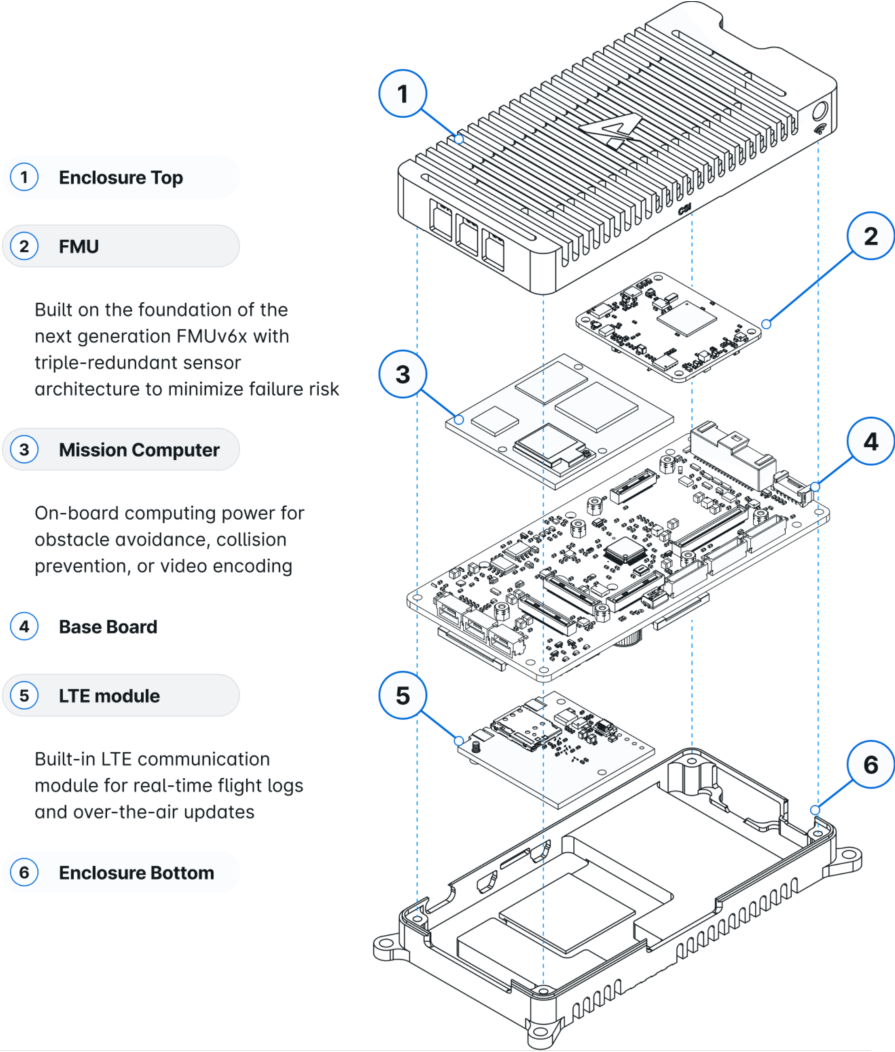
\includegraphics[width=0.8\textwidth]{./img/pdf/skynodeX-datasheet-hw.pdf} 
% %  \includesvg[width=1.0\textwidth]{./img/virtualization.svg} 
%   %\caption[Virtualization mind map]{Virtualization mind map}%
%   \caption{Auterion Skynode X}%
%   \label{fig:skynode-x-hw}
% \end{figure}
%
The mission computer comprises a ARM Cortex-A53 Quad core \gls{cpu} running at
1.8 GHz and two embedded \glspl{gpu} -- GCNanoUltra for 3D acceleration and GC320 for
2D acceleration -- with 4 GB \gls{ram} and 16 GB (\gls{emmc}) + 128 GB (internal
\gls{sd} card) of storage~\cite{skynodeXDatasheet}. Wi-Fi and Bluetooth 5 can be used for low range
wireless communications and a 4G \gls{lte} module for long range ones. It
contains Ethernet and \gls{usb} 2.0 high-speed interfaces only, as \gls{usb} 3.0 usage is discouraged
due to \gls{gps} interference~\cite{skynodeXDatasheet}.
The mission computer runs Auterion
\gls{os} (Linux-based), which communicates with the Autopilot via a proprietary
\gls{sdk} (Auterion \gls{sdk})~\cite{skynodeX-px4}.
%
It supports multicopter, \gls{vtol} airplane and airplane vehicles with a
takeoff weight of up to 500 kilograms. The price tag is circa 1900 USD
dollars\cite{skynodePrice}.

Auterion also announced in June 2024, a compact, low-cost version -- the
Auterion Skynode S -- integrating the \gls{fmu} and mission computer in a 49 x
37 millimeters footprint~\cite{skynodeS-pressRelease}. It features the FMUv6x
flight management unit from the current Skynode X family and a powerful mission
computer with a dedicated 2.3 \gls{tops} \gls{npu} for \gls{ai} and computer
vision applications~\cite{skynodeS-pressRelease}.
%
% \begin{figure}[!hbt]
%   \centering
%   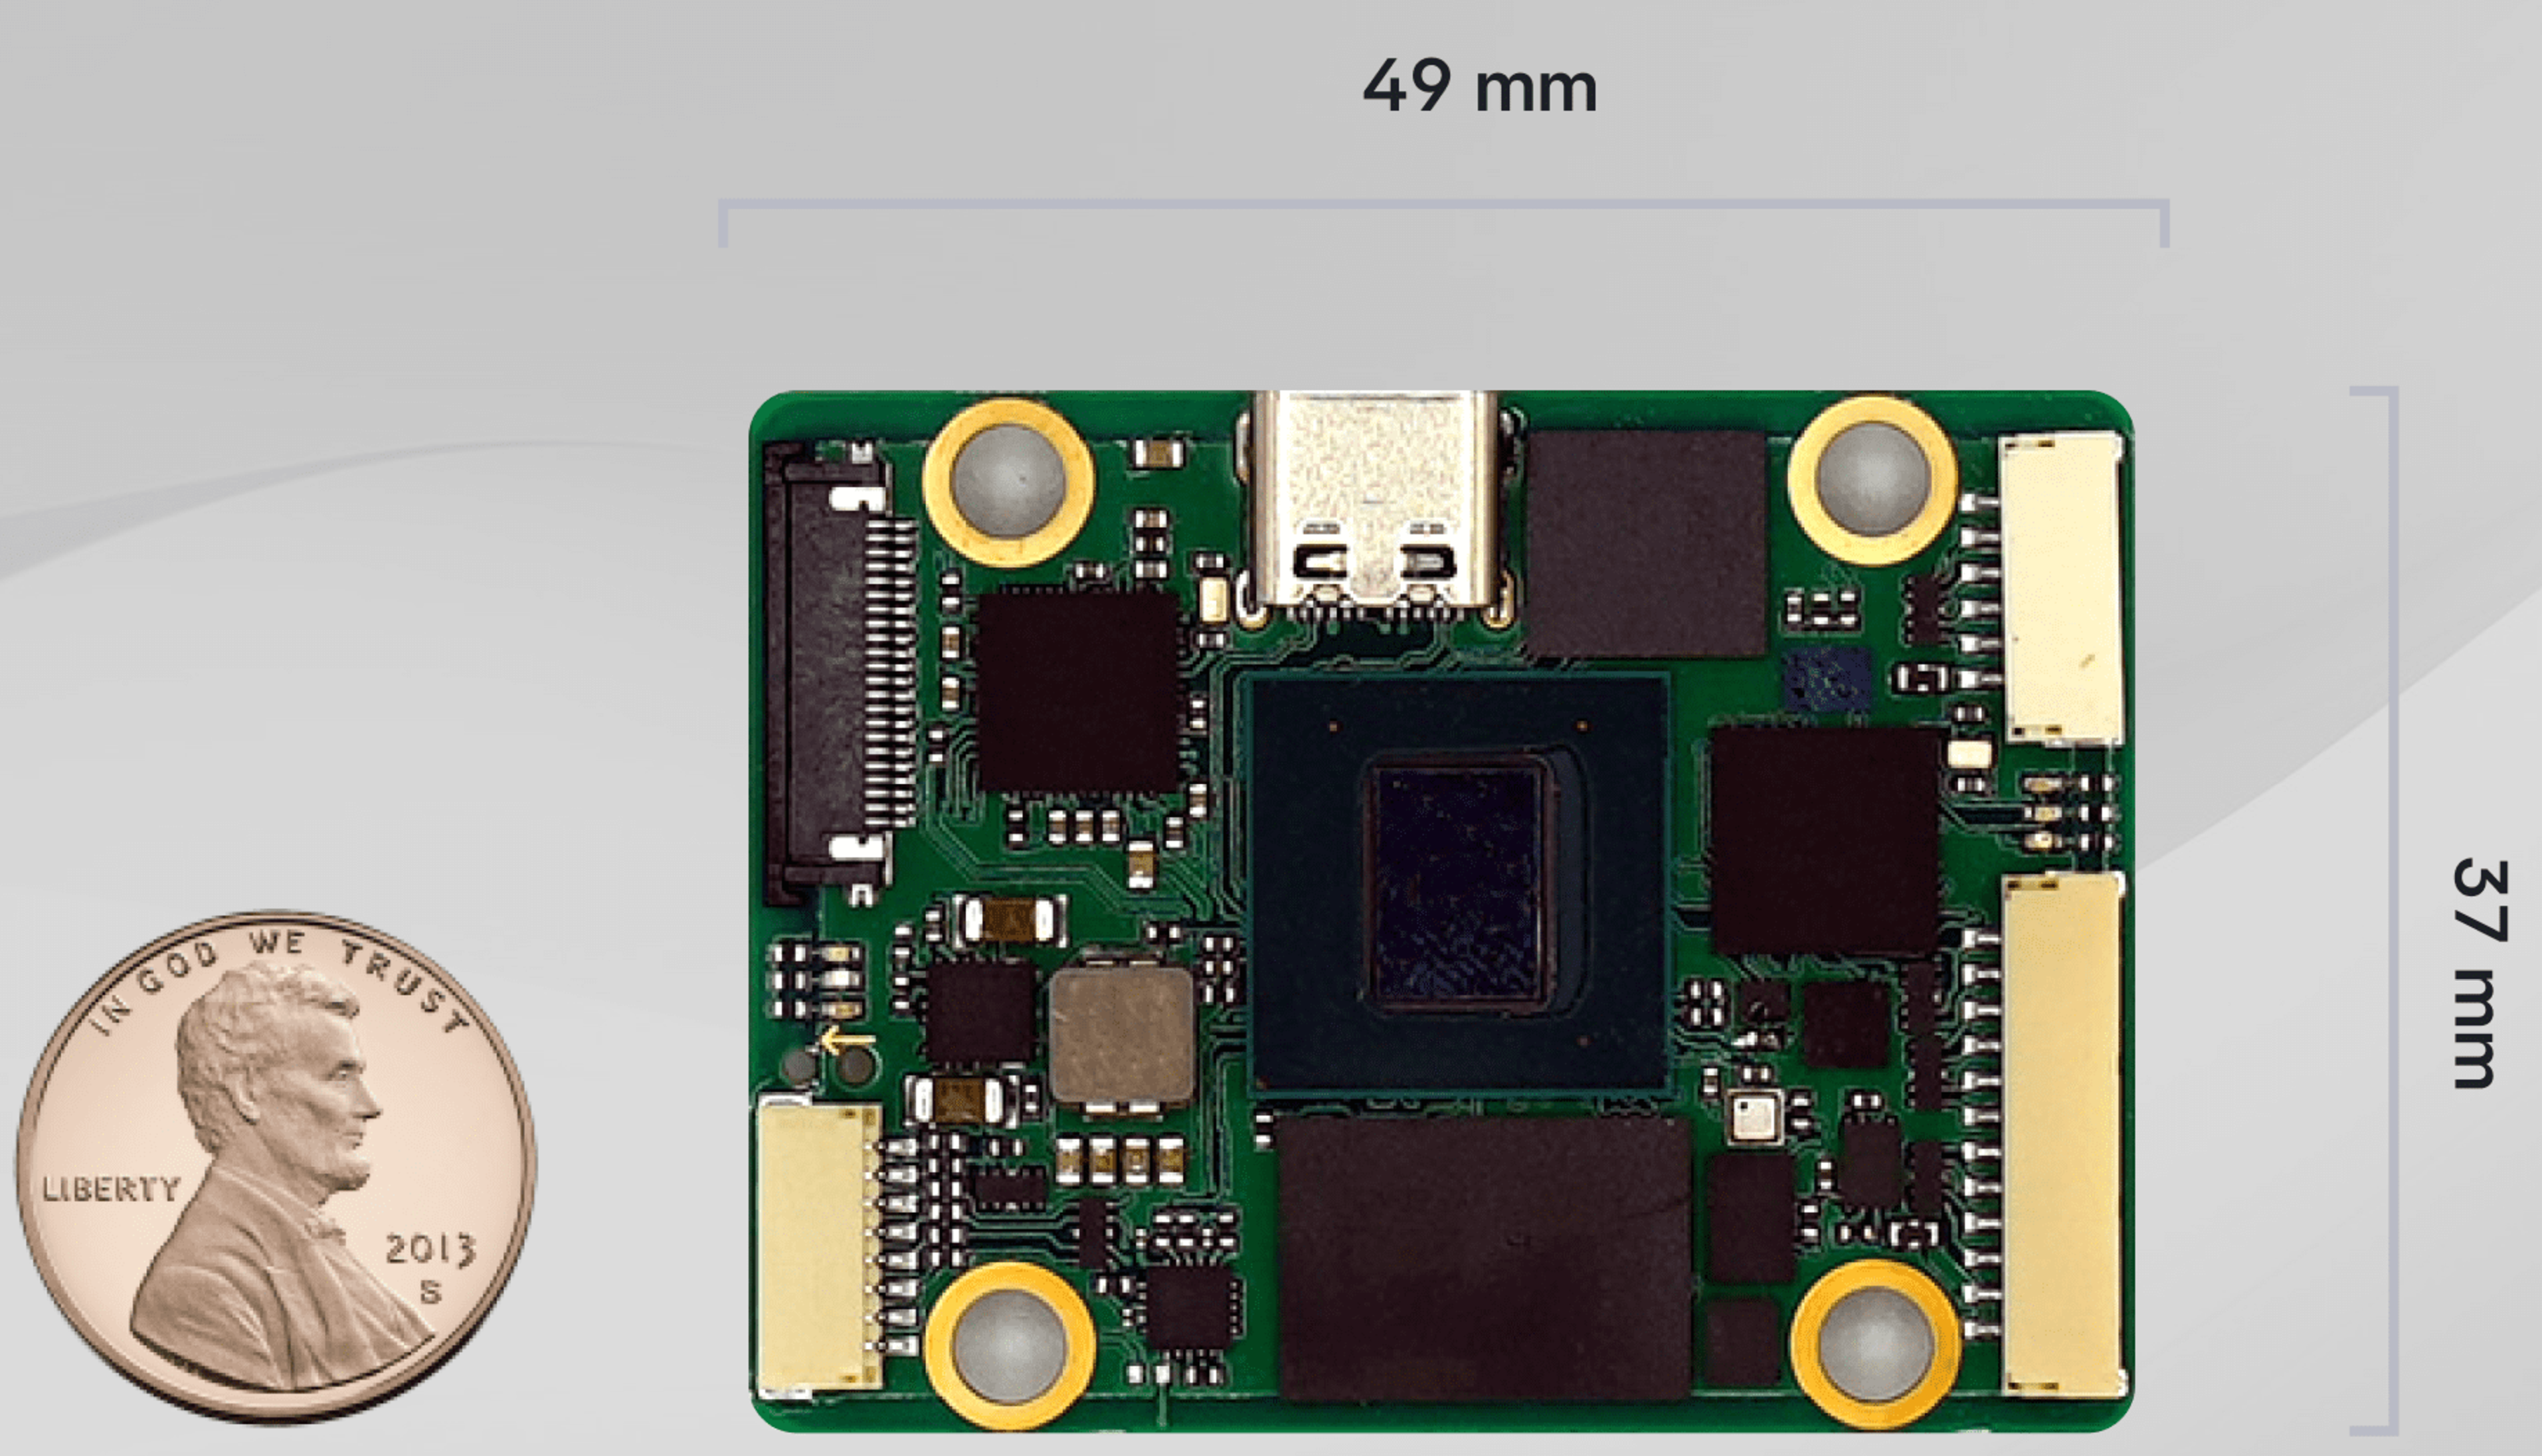
\includegraphics[width=0.8\textwidth]{./img/pdf/skynodeS-hw.pdf} 
% %  \includesvg[width=1.0\textwidth]{./img/virtualization.svg} 
%   %\caption[Virtualization mind map]{Virtualization mind map}%
%   \caption{Auterion Skynode S}%
%   \label{fig:skynode-s-hw}
% \end{figure}
%
The \gls{ai} capabilities of the Skynode S enabled the deployment of a
autonomous target tracking system, even for moving targets, which has proven its resilience against
\gls{gps} jamming or denial of service~\cite{skynodeS-noJamming}. This enabled
Ukraine to face the Russian electronic warfare, and increasing the probability
of mission's success from 20\% to 90\%~\cite{skynodeS-noJamming-2}.
%
Table~\ref{tab:hw-ref} summarizes the \gls{uav} reference hardware.
      % >{\raggedright\arraybackslash}p{1.5cm}  % Platform
      % >{\raggedright\arraybackslash}p{1.2cm}  % Type
      % >{\raggedright\arraybackslash}X         % Notes (flex)
      % >{\raggedright\arraybackslash}p{2.1cm}  % Software
      % >{\raggedright\arraybackslash}p{2.4cm}  % Sensors
      % >{\raggedright\arraybackslash}p{2.4cm}  % Interfaces
      % >{\raggedright\arraybackslash}p{1cm}  % Specs.
      % >{\raggedright\arraybackslash}p{1cm}  % Refs.
\begin{table}[!htbp]
  \centering
  \caption{UAV hardware reference summary}
  \label{tab:hw-ref}

  %---- Local settings (this table only) ----
  \begingroup
    \setlength{\tabcolsep}{3.5pt}   % tighter columns (default ~6pt)
    \renewcommand{\arraystretch}{1.05}
    \scriptsize                    % use \footnotesize if you prefer

    % 7 columns total: 6 fixed p{..} widths you can edit, 1 flexible X for Notes
    % Order: Platform, Type, Specs., Software, Sensors, Interfaces, Notes
    \begin{tabularx}{\textwidth}{@{}
      >{\raggedright\arraybackslash}p{2.2cm}  % Platform
      >{\raggedright\arraybackslash}p{1.2cm}  % Type
      >{\raggedright\arraybackslash}X  % Specs.
      >{\raggedright\arraybackslash}p{2.1cm}  % Software
      >{\raggedright\arraybackslash}p{2.4cm}  % Sensors
      >{\raggedright\arraybackslash}p{2.4cm}  % Interfaces
      >{\raggedright\arraybackslash}p{1cm}         % Notes (flex)
    @{}}
      \toprule
      \textbf{Platform} & \textbf{Type} & \textbf{Specifications} & \textbf{Software} &
      \textbf{Sensors} & \textbf{Interfaces} & \textbf{Notes} \\
      \midrule

      APM 2.8 & OSH & FMU: ATMega 2560 & ArduPilot & IMU; Magnetometer; Barometer & UART; I2C & D \\
      Pixhawk 4 & OSH & FMU: STM32F765; IO Processor: STM32F100 & PX4 & IMU; Magnetometer; Barometer; GPS & SPI; I2C; CAN; UART & \mbox{~} \\
      CC3D Revo & OSH & FMU: STM32F405RGT6 & LibrePilot; ArduPilot & IMU; Magnetometer; Barometer & SPI; I2C; UART; CAN; USB; RF Modem & D \\
      Paparazzi Chimera & OSH & FMU: STM32F767 & Paparazzi UAS & IMU; Barometer & SPI; I2C; CAN; UART; XBEE; USB & \mbox{~} \\
      CUAV v5 Plus & OSH & FMU: STM32F765 & PX4 & IMU; Magnetometer; Barometer & SPI; I2C; CAN; UART & \mbox{~} \\
      Erle-Brain 2 & OSH & FMU + CC: Raspberry Pi 3 & Linux + ArduPilot; PX4 & IMU; Magnetometer; Barometer; temperature & SPI; I2C; UART; USB; Ethernet; Bluetooth & D \\
      PXFMini & OSH & FMU + CC: Raspberry Pi Zero & Linux + PX4 & IMU; Magnetometer; Barometer & I2C; UART & D \\
      PilotPi & OSH & FMU + CC: Raspberry Pi 2/3/4 & Linux + PX4 & IMU; Magnetometer; Barometer & SPI; I2C; UART; USB; Ethernet; Bluetooth; Wi-Fi; CSI & E \\
      HobbyKing KK2 & C & FMU: ATMega 644PA & KK2 & IMU; Magnetometer; Barometer & \mbox{~} & D \\
      SPRacing H7 Extreme & C & FMU: STM32H750 & PX4; Betaflight; Cleanflight & IMU; Barometer & SPI; I2C; UART; IR; USB & \mbox{~} \\
      Aerotenna OcPoc-Zynq Mini & C & FMU + CC: Dual-Core Arm A9; IO: Artix-7 FPGA with 28K logic cells & Linux + PX4 & IMU; Barometer & SPI; I2C; UART; USB; CSI; CAN & D \\
      Navio2 & C & FMU + CC: Raspberry Pi 3; RC I/O coprocessor & Linux + PX4; ArduPilot & IMU; Barometer & SPI; I2C; UART; USB; GNSS & \mbox{~} \\
      PixC4-Jetson & C & FMU: STM32H743; IO Processor: STM32F103; CC: Nvidia Jetson & ArduPilot; PX4 & IMU; Magnetometer; Barometer & SPI; I2C; UART; CAN; USB; Ethernet & \mbox{~} \\
      Auterion Skynode X & C & FMU: STM32H753; IO Processor: STM32F103; CC: Quad-core Arm Cortex-A53 & APX4 & IMU; Magnetometer; Barometer & SPI; I2C; UART; CAN; Ethernet; Wi-Fi; Bluetooth; LTE module & \mbox{~} \\
      Auterion Skynode S & C & FMU: Arm Cortex-M7; CC: Quad-core Arm Cortex-A53; NPU: 2.3 TOPS & APX4 & IMU; Magnetometer; Barometer & SPI; I2C; UART; CAN; CSI; USB & A \\

      \midrule
      \multicolumn{7}{c}{\footnotesize OSH: Open-Source Hardware; C: Commercial; D: Discontinued; E: Experimental; A: AI-capable} \\
      \bottomrule
    \end{tabularx}
  \endgroup
\end{table}
% \FloatBarrier

% %\subsubsection{Gap analysis}%
% \label{sec:gap-analysis-hw}
% Comparison between the open-source and commercial solutions

% \begin{table}[h]
% \centering
% \small
% \caption{UAV Hardware Gap Analysis}
% \label{tab:hw-gap-analysis}
% \begin{tabularx}{\textwidth}{|l|X|X|X|}
% \hline
% \textbf{Dimension} & \textbf{Open-Source Solutions} & \textbf{Commercial Solutions} & \textbf{Gap} \\
% \hline
% Transparency & Full hardware design disclosure (schematics, BOM, PCB layouts) & Proprietary designs with limited disclosure & Open-source provides full auditability; commercial lacks transparency \\
% \hline
% Processor Architecture & ARM-based MCUs (Cortex-M7/M3 @ 216-400MHz) & Mixed: MCUs, FPGA+ARM SoCs, or integrated mission computers (Quad-core A53 + NPU) & Commercial offers higher compute diversity (FPGA/NPU) \\
% \hline
% Memory & Limited (2MB Flash/512KB RAM max) & Expanded resources (4GB RAM + 128GB storage in Skynode) & Commercial solutions offer >100× memory capacity \\
% \hline
% Sensors & Basic IMU/barometer/magnetometer & Advanced redundancy (triple IMU/GPS) and AI-capable sensors & Commercial enables fault tolerance and AI processing \\
% \hline
% Connectivity & UART/SPI/I²C/CAN & Enterprise features: LTE, VPN, Ethernet switches & Commercial provides industrial-grade networking \\
% \hline
% AI Capabilities & None & Dedicated NPUs (2.3 TOPS) for computer vision & Commercial enables edge AI for GPS-denied navigation \\
% \hline
% Power Management & Not specified & Triple-redundant power systems & Commercial prioritizes fail-safe power \\
% \hline
% Price & Low-cost (COTS components) & Premium pricing (\$1,900 for Skynode X) & 10-100× cost difference \\
% \hline
% License & Permissive (BSD) or restrictive (GPL) & Proprietary or OSS-based proprietary extensions & Commercial leverages permissive licenses for closed ecosystems \\
% \hline
% Target Market & Academic/hobbyist & Enterprise/military & Commercial focuses on mission-critical applications \\
% \hline
% \end{tabularx}
% \end{table}

\subsection{UAV Reference Software}%
\label{sec:uav-ref-sw}
In this section we discuss the reference software for \glspl{uav}.
Firstly, we present an overview over the software architecture. Then, we analyze
in more depth the open-source and commercial software solutions for \glspl{uav}.

\subsubsection{Overview and Architecture}%
\label{sec:overv-arch-sw}
Fig.~\ref{fig:uav-sw-arch} illustrates the high-level abstraction of the
most common structure of \gls{uav} software
architecture~\cite{leccadito2018survey,px4-sysArch}.
%
The main computing platforms are depicted in orange: (1) the flight controller
or \gls{fmu} (e.g., Pixhawk); (2) the \gls{gcs} (e.g., a desktop/laptop computer);
(3) and, optionally, the companion computer (e.g., a Raspberry Pi).
The companion computer provides additional features, but crucial for autonomous
flights, such as collision avoidance and prevention, odometry or payload control
(camera, \gls{lidar}, etc.). Furthermore, the companion computer can assist in
the \gls{uav}'s navigation in \gls{gps}-denied and/or communications-denied
environments, using \gls{ai}-based software components (e.g., Auterion
Skynode~\cite{skynodeS-noJamming}).
%
The physical hardware is depicted in purple (sensors, actuators, and payload),
while the layers of the software stack are shown in green. The arrows indicate the communication link and
associated protocols.

% UAV SW Arch
\begin{figure}[!hbt]
  \centering
  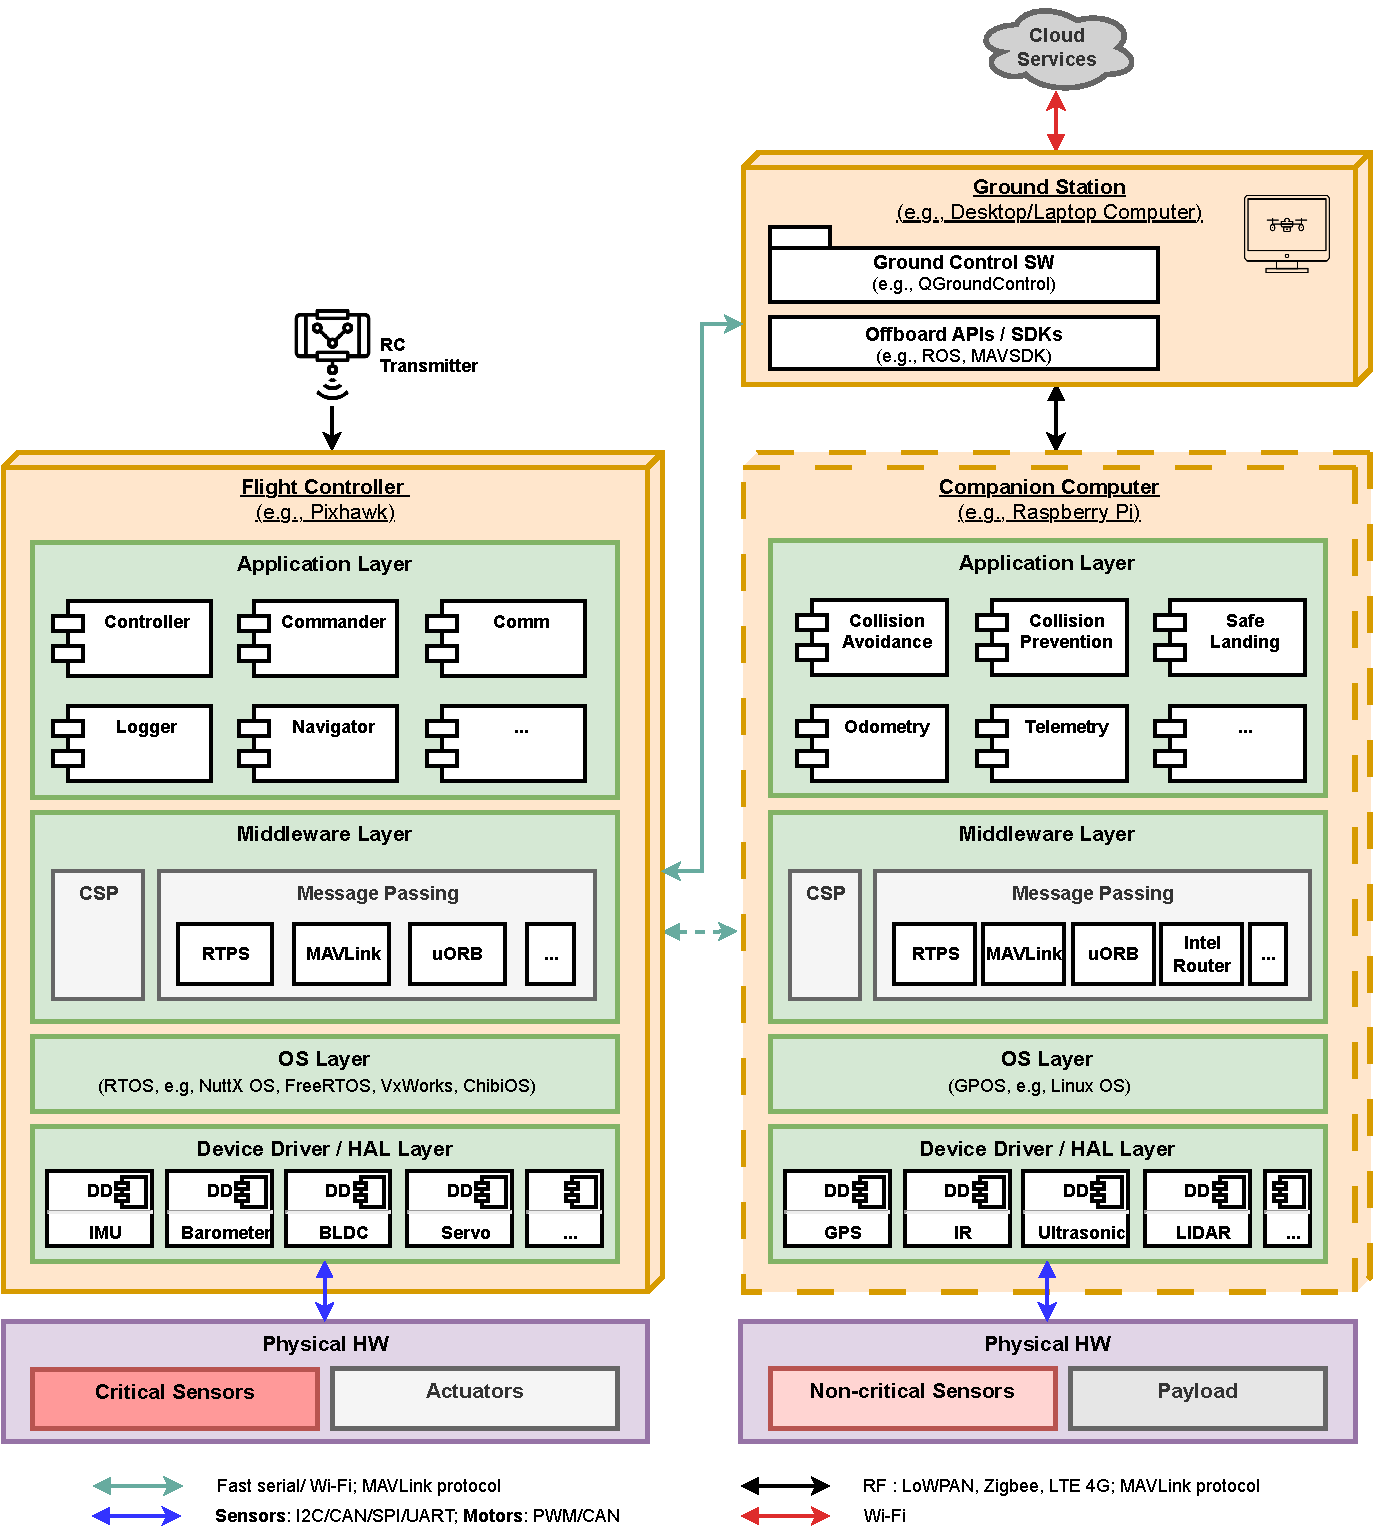
\includegraphics[width=1.0\textwidth]{./img/pdf/uav-sw-arch.pdf} 
%  \includesvg[width=1.0\textwidth]{./img/virtualization.svg} 
  %\caption[Virtualization mind map]{Virtualization mind map}%
  \caption{UAV SW architecture: most common structure}%
  \label{fig:uav-sw-arch}
\end{figure}

The flight controller and companion computer software stack structure is
similar, and is comprised of four layers:

\begin{enumerate}
\item \textbf{Application Layer}: this layer is where the applications/tasks
  reside, providing the high-level functionalities of the system. In the flight
  controller we have the critical tasks, namely,
  \emph{Controller}, \emph{Commander}, \emph{Navigator}, \emph{Logger},
  or \emph{Communications}, and in the companion computer the secondary tasks,
  providing mission and navigation extra features, such as, \emph{Collision
    Avoidance}, \emph{Collision Prevention}, \emph{Safe Landing},
  \emph{Odometry}, and \emph{Telemetry}.
%
\item \textbf{Middleware Layer}: the middleware is an intermediate layer,
  responsible for abstracting the interface with the \gls{os} and the
  communications through message passing --- using real-time and or asynchronous
  protocols, such as \gls{rtps}, MAVLink, or \gls{uorb} --- and for providing
  an extra layer of security enforcing \gls{csp} mechanisms. The flight
  controller communicates with the \gls{gcs} through a Wi-Fi connection and
  optionally with the Companion Computer through a fast serial/Ethernet
  connection.
%
\item \textbf{\gls{os} Layer}: the \gls{os} provides the basic services for
  system's operation and a straightforward environment for application's
  development. The flight controller hosts a \gls{rtos} to meet the stringent
  requirements and deadlines of the \gls{uav}'s control, such as,
  \lstinline{NuttX}, \lstinline{FreeRTOS}, \lstinline{VxWorks}, and \lstinline{ChibiOS}. On
  the other hand, the companion computer hosts a \gls{gpos}, as the applications
  on top have soft real-time requirements. Furthermore, it provides a much
  better bootstrapping environment for ``general'' software development than a
  \gls{rtos}, e.g., \gls{ros}-based avoidance libraries are available for Linux~\cite{px4-sysArch}.
%
\item \textbf{Device Driver Layer (\gls{hal})}: this layer abstracts the
  underlying hardware, providing a tractable interface for the \gls{os} for data
  acquisition and motors' actuation.
\end{enumerate}

The \gls{gcs} software (e.g., \emph{QGroundControl}) typically runs on a desktop/laptop computer or mobile
device providing real-time monitoring of the flight superimposed on a map and
\gls{uav}'s control functionalities, communicating directly with the flight
controller or indirectly via companion computer. The
software interface between both systems is achieved through the use of off-board
\glspl{api} or \glspl{sdk}, like \gls{ros} or MAVSDK~\cite{px4-sysArch}. 

\subsubsection{Open-source solutions}%
\label{sec:open-source-solut-sw}
\glsxtrfull{oss} solutions, like their hardware counterparts, have been
developed to provide more transparency, flexibility, and
maintainability, while trying to be cost-effective. \gls{oss} means that the
software's source code is released under free/libre
terms~\cite{freeGNU}. The most prominent \gls{oss} autopilots at the moment are
\lstinline{PX4}~\cite{px4-github},
\lstinline{ArduPilot}~\cite{arduPilot-github},
\lstinline{Paparazzi UAS}~\cite{paparazzi-github}, and \lstinline{INAV}.
Other flight-control software, such as
\lstinline{Betaflight}~\cite{betaflight-github},
\lstinline{Cleanflight}~\cite{cleanflight-github},
\lstinline{Crazyflie}~\cite{crazyflie-home}, and \lstinline{LibrePilot}~\cite{librePilot-arch} targets the \gls{fpv} racing
market and assumes expert manual piloting skills. In this context, manual
control is the priority, so autopilot features are generally unnecessary and not
supported.
\lstinline{LibrePilot} runs on the FreeRTOS \gls{rtos} but is not actively
maintained~\cite{librePilot-github}, whereas \lstinline{Betaflight},
\lstinline{Cleanflight}, and \lstinline{Crazyflie} run directly on the board.

% \paragraph{PX4}
%
\lstinline{PX4} is an autopilot flight stack for \glspl{uv}, with a strong focus on the
\glspl{uav}. Started in 2012 and released under
a permissive \gls{bsd}-2 license~\cite{px4-github}, it is widely used in
industrial and commercial domains
\lstinline{PX4}~\cite{skynodeX-px4,spRacing-px4}. Like ArduPilot, it supports a
broad range of \gls{uav} airframes and other \glspl{uv}.
%
PX4 is loaded onto
the flight controller hardware using the \emph{QGroundControl}
application and runs atop of the NuttX OS, although ROS support is also
available~\cite{jargalsaikhan2022architectural}. \emph{QGroundControl} is also
used to configure PX4 and interface the flight controller, and an \gls{rc} unit
can be used to manually control the drone.
%
PX4 uses the MAVLink protocol to communicate with the flight controller and the
\gls{uorb} message \gls{api} for data transfer between its internal
modules~\cite{px4-sysArch,jargalsaikhan2022architectural}. It requires an
\gls{imu}, magnetometer and barometer for manual modes, but for autonomous
missions a \gls{gps} must be used. Flight logs are generated upon takeoff and
can be analyzed to assess the flight behavior using \emph{Flight Review}, or
\emph{Px4Tools}~\cite{glossner2021overview}. 

%\paragraph{ArduPilot}
%
\lstinline{ArduPilot} is another autopilot flight stack for \glspl{uv}, also with a strong focus
on \glspl{uav}. Started in 2009, it was released under the more restrictable
\gls{gpl}v3 license~\cite{arduPilotHistory}. It supports the \emph{Linux} and
\emph{ChibiOS} operating
systems~\cite{arduPilot-github,jargalsaikhan2022architectural} and runs on a large number of
\gls{osh} platforms such as \emph{Pixhawk}.
%
ArduPilot features, like PX4~\cite{px4-features}, include:
multiple flight modes (manual, semi- and full-autonomous) with multiple
stabilization options; programmable missions with 3D waypoints and optional
geofencing; support for multiple sensors and buses; fail-safe actions and
support for navigation in \gls{gps} denied environments~\cite{arduPilot-home}.
%
ArduPilot supports the MAVLink protocol for communication with
\glspl{gcs} and companion computers~\cite{arduPilot-home}. Mission commands are
stored in \gls{eeprom} and executed one-by-one when the vehicle is switched into
\emph{Auto} mode~\cite{ardupilot-mavlink}.

% \paragraph{Paparazzi UAS}
%
\lstinline{Paparazzi UAS} is the oldest autopilot flight stack for drones
currently active. Started in 2003, it was released under the \gls{gpl}v2
license, supporting different \gls{uav}'s airframes~\cite{paparazzi-home}.
It runs atop of the \emph{ChibiOS} operating
system~\cite{paparazzi-sysOverv} and uses its own \emph{PPRZLINK} protocol for communication
with \glspl{gcs} and companion computers~\cite{paparazzi-sysOverv}, transferring
data between the modules via the proprietary middleware \emph{AirBorne Ivy}
\gls{abi}~\cite{jargalsaikhan2022architectural}.

Derived from \lstinline{Cleanflight}, \lstinline{iNAV} is an open-source
autopilot firmware for multirotors, fixed-wing aircraft, and rovers that require
\gls{gps}-assisted flight rather than acro/racing~\cite{inav-github}. It sits
between racing-oriented \lstinline{Betaflight} and full-autonomy stacks such as
\lstinline{ArduPilot}, providing navigation features like position/altitude
hold, return-to-home, and waypoint missions configured via the \lstinline{iNAV}
Configurator~\cite{inav-github}. The hardware support is restricted to a few
controllers, notably STM32 F4/F7/H7 and AT32 families~\cite{inav-github}.

% \paragraph{}
% Fig.~\ref{fig:uav-sw-arch-oss-compar} shows the software
% stack layers and modules for the aforementioned \gls{oss} solutions and for
% \emph{mpFCS}, the portable \gls{fcs} developed by Jargalsaikhan et
% al.~\cite{jargalsaikhan2022architectural}.

% % UAV SW Arch OSS Comparison
% \begin{figure}[!hbtp]
%   \centering
%   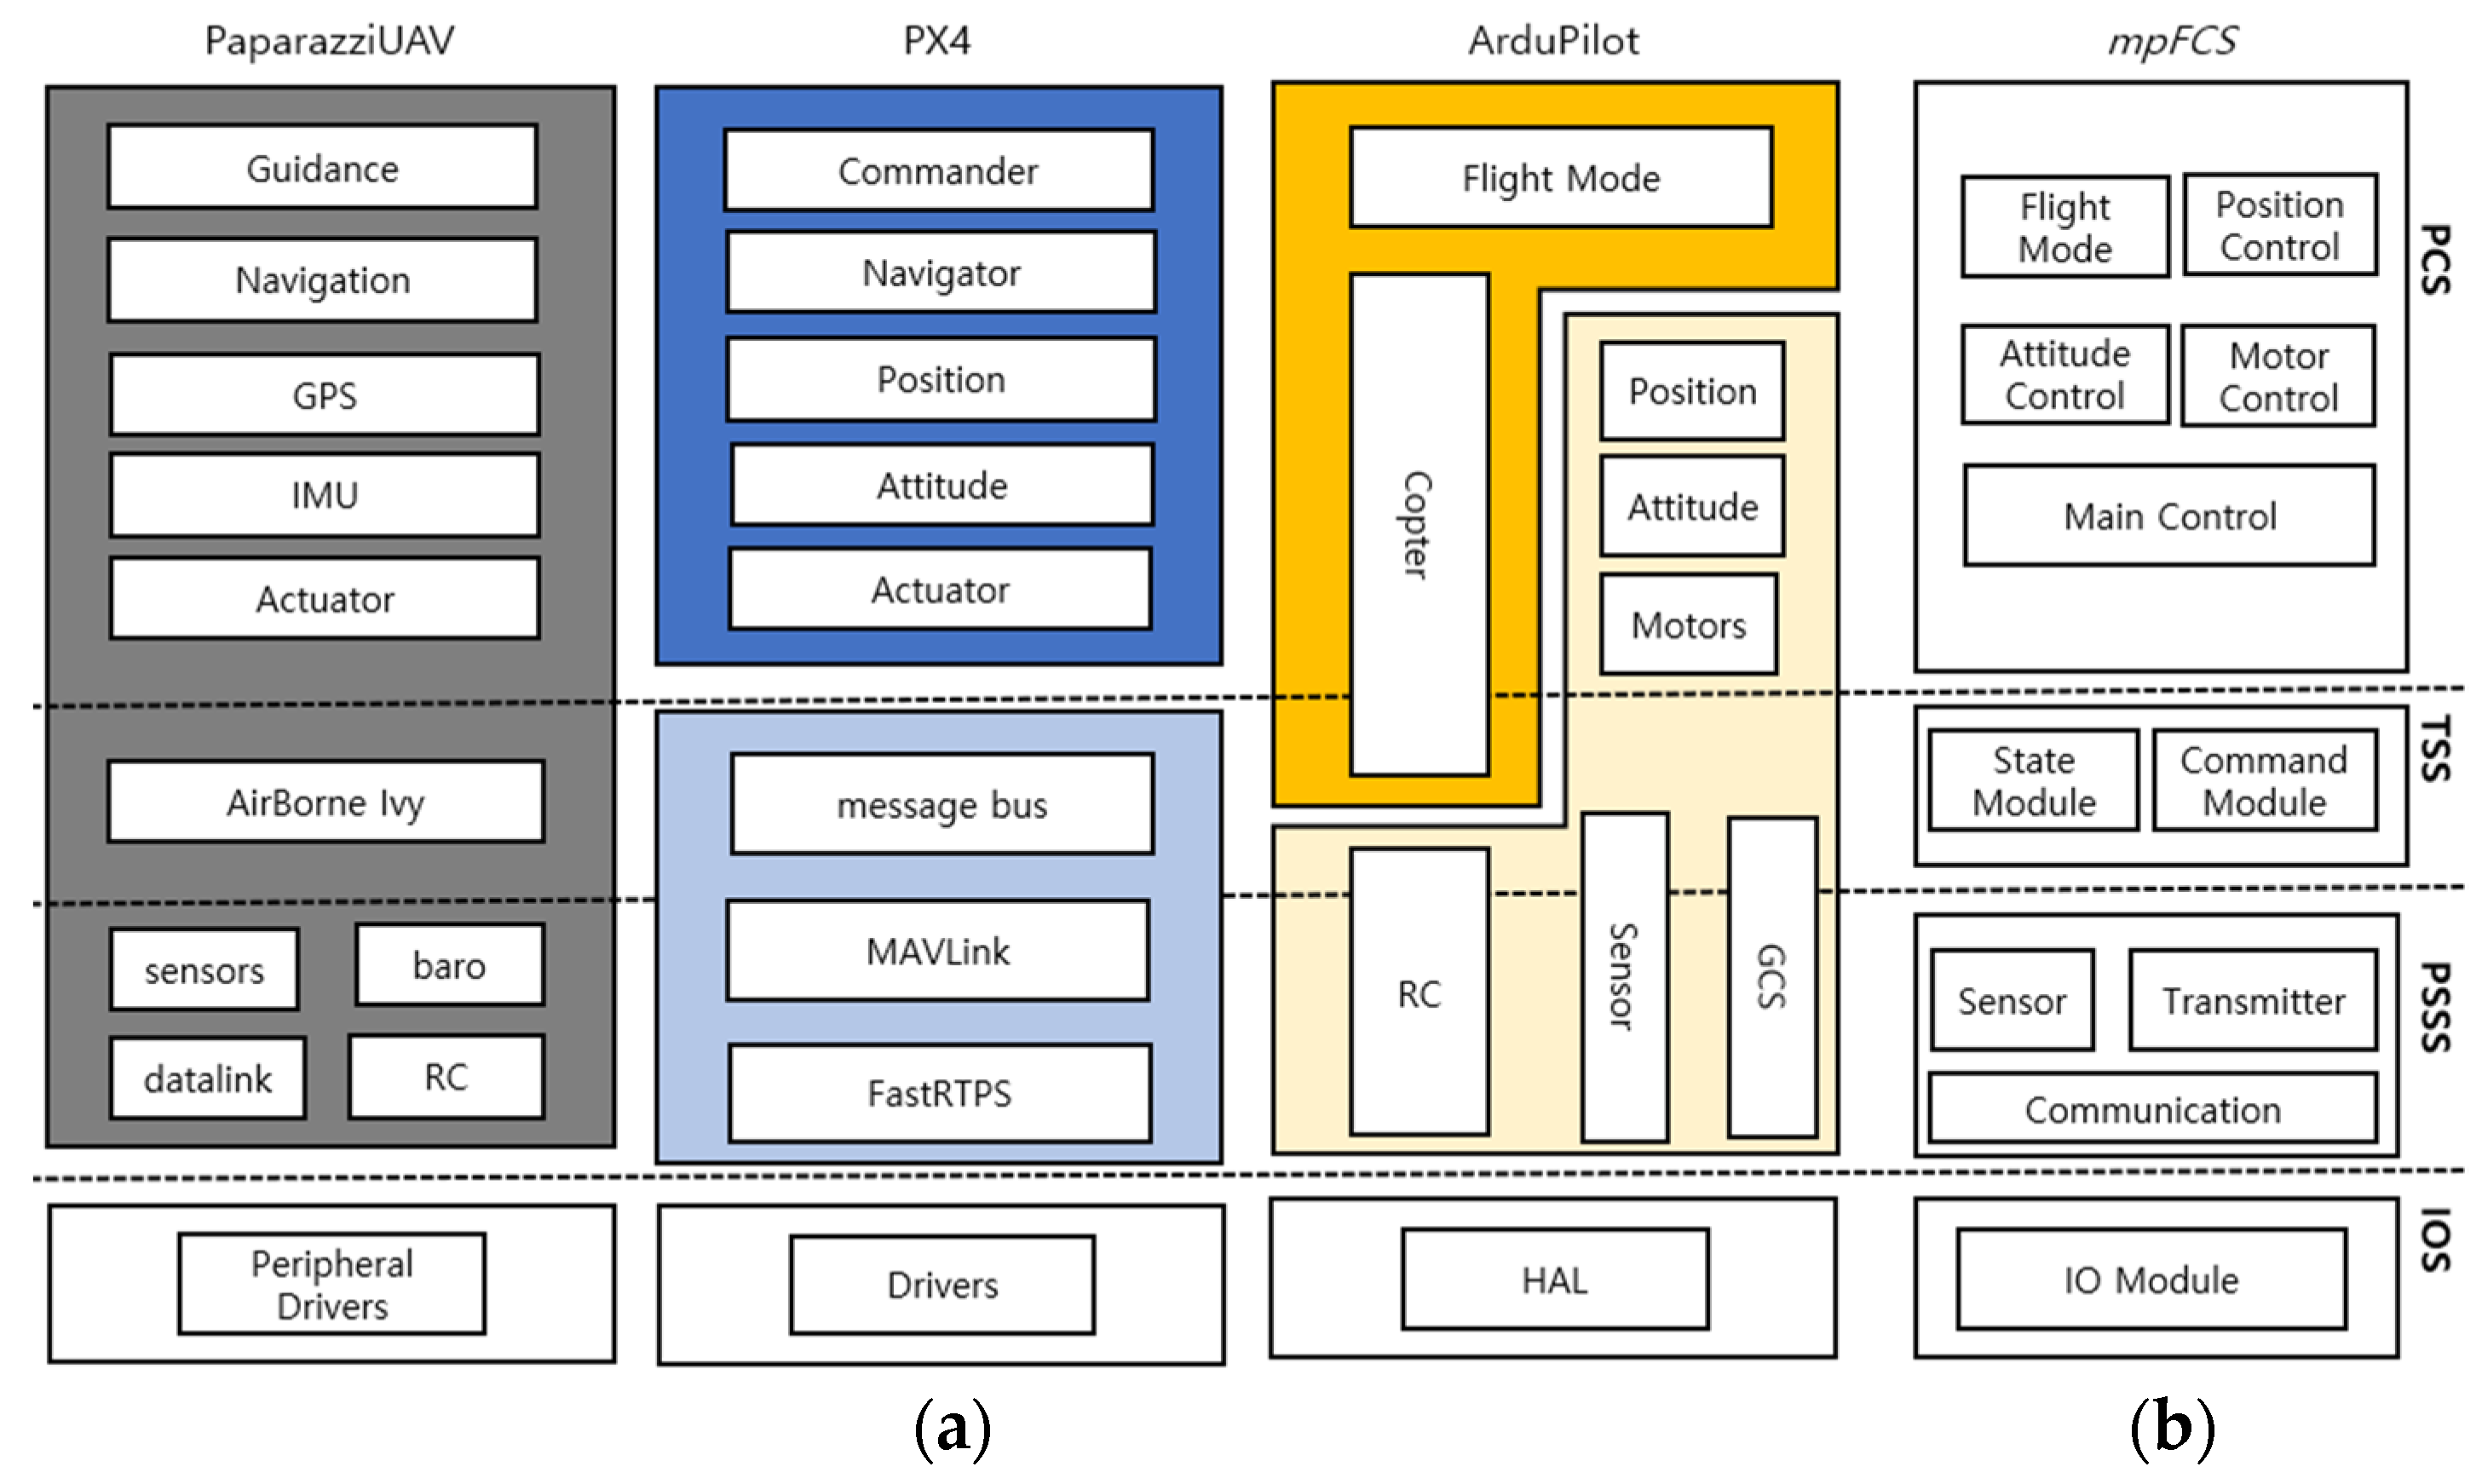
\includegraphics[width=0.8\textwidth]{./img/png/uav-sw-arch-oss.png} 
% %  \includesvg[width=1.0\textwidth]{./img/virtualization.svg} 
%   %\caption[Virtualization mind map]{Virtualization mind map}%
%   \caption[Analysis of the OSS modules and the mpFCS]{Analysis of the OSS
%     modules and the mpFCS:~(a) OSS (Paparazzi UAS, PX4, ArduPilot); (b) mpFCS~\cite{jargalsaikhan2022architectural}\footnotemark}%
%   \label{fig:uav-sw-arch-oss-compar}
% \end{figure}
%  % TODO: get license
% \fnlicReq{MDPI}{5457890117132}%

% \enlargethispage{\baselineskip}

% \clearpage % or \newpage

\subsubsection{Commercial solutions}%
\label{sec:commercial-solutions-sw}
Typically, the commercial proprietary solutions do not disclose information
about the product. They provide extensibility through the use of
\glspl{sdk}, like the Dji~\cite{djiSDK} or the Parrot drones\cite{parrot-sdk}, enabling the end-user to use
extra features, but requires specialized knowledge.
%
On the other hand, some commercial solutions can explore
more permissible \gls{oss} licenses, like the \gls{bsd} license provided by PX4,
to add extra functionalities and bundle it as a closed, commercial,
product. This is exactly the case for the Auterion PX4 (PX4) autopilot, a
enterprise-hardened autopilot that runs on the Auterion \glspl{fmu}.
Fig.~\ref{fig:uav-sw-arch-auterion} illustrates the Auterion software stack.

% UAV SW Arch
\begin{figure}[!hbt]
  \centering
  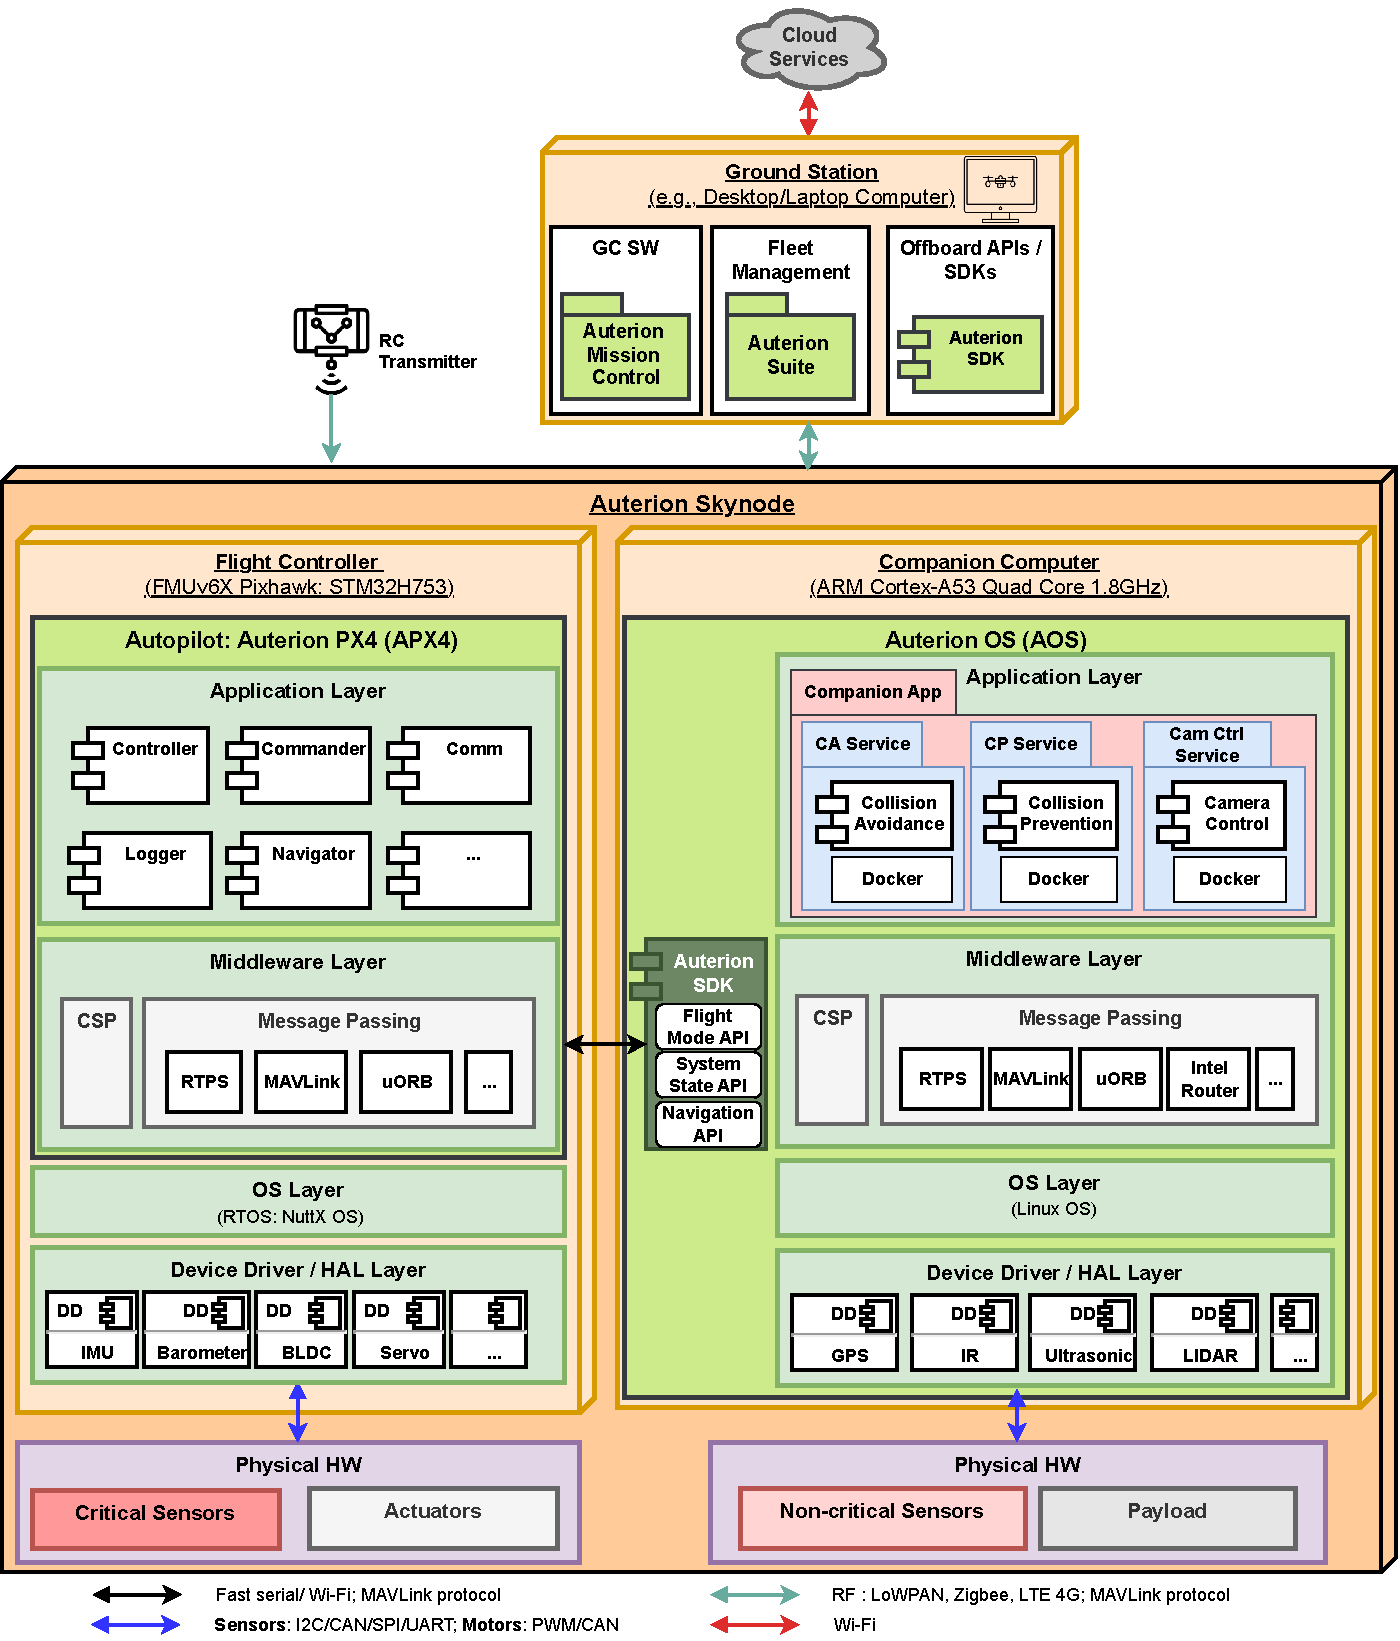
\includegraphics[width=0.9\textwidth]{./img/pdf/uav-main-sw-arch-auterion.pdf} 
%  \includesvg[width=1.0\textwidth]{./img/virtualization.svg} 
  %\caption[Virtualization mind map]{Virtualization mind map}%
  \caption{UAV SW architecture: Auterion software stack}%
  \label{fig:uav-sw-arch-auterion}
\end{figure}

The \lstinline{Auterion Skynode} combines the an FMUv6X-based Pixhawk
\gls{fmu} and the companion/mission computer into a single board~\cite{auterion-sw}. The flight
controller runs the autopilot stack (APX4) on top of the NuttX \gls{rtos}
licensed under the Apache 2.0 license which allows for proprietary reuse. The
mission computer runs the Auterion \gls{os} (AOS), a customized embedded Linux
\gls{os}, to support additional features, like collision avoidance and
prevention, odometry, or camera control~\cite{auterion-sw}. These additional features or services,
are containerized in a Docker image to increase isolation and enable easy and
fast system update, minimizing the dependencies. However, to optimize storage
requirements, developers are instructed to: (1) package these services into a
single application (e.g., \lstinline{Companion App}), ensuring the user only needs to handle a single
\lstinline{.auterionos} file; (2) write a common base \lstinline{Dockerfile} for
a shared environment for the deployed services~\cite{auterion-sw-services}. Thus, AOS software development
follows the microservices architecture based on the Docker technology.
The AOS' applications can query the autopilot or issue commands to it using the
provided \glspl{api} in the \lstinline{Auterion SDK}.
%
The \lstinline{Auterion Skynode} can be controlled using a \gls{rc} transmitter
or software running on the \gls{gcs}. The \lstinline{Auterion Mission Control}~\cite{auterion-missionControl}
is a ground control software specialized for Auterion vehicles, very similar to
\lstinline{QGroundControl}, enabling the UAV's remote control.
The \lstinline{Auterion Suite}~\cite{auterion-suite} is a fleet management software, providing
real-time information about the UAV, predictive maintenance actions, flight
analysis, and \gls{ota} updates.

If, however, we expand the search to include any proprietary
software component, such as the \lstinline{VxWorks} \gls{rtos} then the results'
list becomes significantly larger, namely, the Northrot Grumman X-47B
\gls{uav}~\cite{vxWorks-uav-northrop}, the Airbus
Helionix~\cite{vxWorks-uav-aribus-helionic}, and the Airbus
Atlante~\cite{vxWorks-uav-aribus-atlante}.
%
Table~\ref{tab:sw-ref} summarizes the \gls{uav} reference software.

% Preamble (needed once in your document)
% \usepackage{booktabs}
% \usepackage{tabularx}
% \usepackage{array}

% Preamble (once in your doc)
% \usepackage{booktabs}

\begin{table}[t]
  \centering
  \caption{UAV reference software summary}
  \label{tab:sw-ref}

  % ---- local-only sizing/spacing ----
  \begingroup
  \footnotesize
  \setlength{\tabcolsep}{4pt}      % tighter column padding
  \renewcommand{\arraystretch}{1.05}% slightly tighter rows

  \begin{tabular}{@{} l l l c l @{}}
    \toprule
    \textbf{FCS} & \textbf{License} & \textbf{OS} & \textbf{Autopilot} & \textbf{Notes} \\
    \midrule
    ArduPilot     & GPL~3        & ChibiOS; Linux & Yes & \\
    PX4           & BSD~3        & NuttX; Linux   & Yes & \\
    Paparazzi UAS & GPL~2        & ChibiOS        & Yes & \\
    Crazyflie     & GPL~3        & Baremetal      & No  & Racing \\
    Betaflight    & GPL~3        & Baremetal      & No  & Racing \\
    CleanFlight   & GPL~3        & Baremetal      & No  & Racing \\
    KK2           & GPL~3        & Baremetal      & No  & Not maintained \\
    LibrePilot    & GPL~3        & FreeRTOS       & No  & Not maintained \\
    iNAV          & GPL~3        & Baremetal      & Yes & \\
    Dji           & Proprietary  & ND             & Yes & Provides SDK \\
    Parrot        & Proprietary  & ND             & Yes & \\
    APX4          & Proprietary  & NuttX          & Yes & Provides SDK \\
    \bottomrule
  \end{tabular}

  \endgroup
  % ---- local-only sizing/spacing ends ----
\end{table}

% \subsubsection{Gap analysis}%
% \label{sec:gap-analysis-sw}
% Comparison between the open-source and commercial solutions

% \begin{table}[h]
% \centering
% \small
% \caption{UAV Software Gap Analysis}
% \label{tab:sw-gap-analysis}
% \begin{tabularx}{\textwidth}{|l|X|X|X|}
% \hline
% \textbf{Dimension} & \textbf{Open-Source Solutions} & \textbf{Commercial Solutions} & \textbf{Gap} \\
% \hline
% License & GPL/BSD licenses with source access & Proprietary SDKs or OSS-based closed products & Commercial restricts modification rights \\
% \hline
% Middleware & Custom protocols (uORB, PPRZLINK) & Standardized microservices with Docker containers & Commercial offers modern containerization \\
% % \hline
% % Portability & Limited HAL implementation & Enterprise-hardened portability & Commercial provides production-grade abstraction \\
% \hline
% API Extensibility & ROS/MAVSDK support & Proprietary SDKs with cloud integration & Commercial enables tighter ecosystem control \\
% \hline
% Real-Time Performance & RTOS-based (NuttX, ChibiOS) & Military-grade RTOS (VxWorks) & Commercial offers certified real-time guarantees \\
% \hline
% Update Mechanism & via USB or radio in offline mode & via USB, radio or Wi-Fi; updates with fleet management & Commercial enables remote maintenance \\
% \hline
% Security Features & Basic CSP mechanisms & Container isolation + hardware-enforced security & Commercial provides defense-grade protection \\
% \hline
% AI/ML Integration & Limited (ROS-based libraries) & Native AI stack for target tracking & Commercial enables advanced autonomous behaviors \\
% \hline
% Ecosystem Tools & QGroundControl + Flight Review & Integrated mission control + cloud suites & Commercial offers end-to-end mission lifecycle support \\
% \hline
% Documentation & Partially outdated & Professional technical support & Commercial ensures reliability for critical ops \\
% \hline
% \end{tabularx}
% \end{table}

% ============================================================================
\section{Related Work}
\label{sec:related-work}
% -- GOAL: Survey what exists for trustworthy UAV software stacks,
%    define how you judge “trustworthy,” summarize current flight stacks + platforms,
%    and review virtualization options used onboard. Finish with a tight gap analysis
%    that bridges to your Design/Implementation.

%============================================================
% Scope and criteria (kept inline as you prefer)
We review prior work on UAV flight stacks, onboard platforms, and virtualization
approaches to understand what is required to safely consolidate mixed-critical
workloads on a single platform.
We focus on deployments where flight-control (safety-critical) and
mission/auxiliary functions (non-critical) must coexist with bounded
interference and predictable timing.
We define \emph{trustworthiness} as the conjunction of: (i) temporal, spatial,
and fault-containment isolation with verifiable real-time behavior; (ii)
deterministic execution and analyzable latency budgets; (iii) a small, auditable
\gls{tcb} and a maintainable codebase; (iv) platform fit under SWaP-C
constraints; and (v) openness to enable scrutiny and broad adoption.
We use these criteria to assess prior work throughout this section.
% Where applicable, we
% interpret these dimensions against sector standards (e.g., DO-178C, ISO 26262)
% and UAV-specific device/timing constraints.


%============================================================
\subsection{Flight Control Software Used in Practice}
\label{subsec:rw-flight-stacks}
The most widely used open-source autopilots are PX4, ArduPilot, Paparazzi UAS,
and iNAV.
PX4, widely adopted in industrial and commercial settings, runs on NuttX (and
Linux), offers broad platform coverage, and has a modular architecture.
ArduPilot targets Linux and ChibiOS, with extensive support for \gls{osh}
platforms (e.g., Pixhawk) and rich vehicle types.
Paparazzi UAS, one of the earliest open stacks, runs atop ChibiOS with a strong
fixed-wing heritage.
iNAV sits between racing firmware (e.g., Betaflight) and full autopilots,
emphasizing GPS-assisted flight but supporting only a subset of boards (notably
STM32 F4/F7/H7 and AT32).

Jargalsaikhan et al.~\cite{jargalsaikhan2022architectural} analyzed module-level
portability across PX4, ArduPilot, Paparazzi, and a custom stack, evaluating
structure, messaging, and \gls{hal} design against portability requirements
(simplicity, modularity, centralized messaging, standard interfaces, \gls{hal}
quality, documentation). They found that only \emph{ArduPilot} and \emph{PX4}
provide \glspl{hal} and that \emph{ArduPilot} lacks message
centralization. Moreover, all surveyed systems rely on non-standard messaging,
which hinders portability despite being open source.

In 2021, Wang et al.~\cite{wang_exploratory_2021} conducted an exploratory study
of autopilot software bugs, analyzing 569 fixed issues from PX4 and ArduPilot
and identifying 168 UAV-specific bugs. Root causes spanned eight classes (e.g.,
missing initialization, limit/parameter mishandling, hardware/software-dependent
priority), highlighting recurring pain points. They reported that 39\% of those
bugs pertained to PX4 (with \(\approx\)609~kLOC) versus ArduPilot (\(>1505\)~kLOC), and
that PX4 had more resolved issues overall (\(\approx\)5k vs.\ \(\approx\)3.5k), suggesting
a highly engaged community. Such scrutiny is only possible with open-source
stacks, improving transparency and, by extension, trustworthiness.

Much academic work with PX4 and ArduPilot targets flight
control~\cite{li_embedding_2022,li_plug-and-play_2021,baldi_ardupilot-based_2022,dangelo_efficient_2024}
and simulation-based
verification~\cite{baldi_ardupilot-based_2022,dang_nguyen_vision-based_2019,dai_rflysim_2021},
often to develop adaptive control and to broaden functional test coverage via
\gls{sitl}/\gls{hitl}.
D'Angelo et al.~\cite{dangelo_efficient_2024} explicitly cite PX4's BSD-3
license as enabling code modifications without mandatory upstreaming, helping
companies protect intellectual property.
%

In the commercial domain, flight-control software is typically closed-source,
with extensibility exposed via \glspl{sdk}~\cite{parrot-sdk}. Auterion, by
contrast, maintains a proprietary PX4 fork for the flight controller and deploys mission applications via containers on the companion computer. % NOTE: brief here; full discussion appears later
%
Buquerin~\cite{buquerin2018security} evaluated the
VxWorks~7 \gls{rtos} (commercial, avionics) and reported that basic attacks (e.g., buffer overflows, string vulnerabilities) caused noticeable performance degradation, with no built-in protection against malware or command injection.
This underscores the need for supervising technology (e.g., a hypervisor) to contain faults across domains.

With open-source \glspl{rtos}, transparency increases but isolation is still limited.
Zhang et al.~\cite{zhang2021best} compared NuttX and ChibiOS: ChibiOS generally
outperformed NuttX on timing, avoided priority inversion with mutexes, and
exhibited lower context-switch overhead; NuttX lacks priority inheritance with
mutexes and has a larger codebase.
Thus, an \gls{rtos} alone does not provide the inter-domain isolation required for \glspl{mcs}.

From a mixed-criticality perspective, PX4 and ArduPilot emerge as the most
mature and widely supported open-source autopilots, but non-standard messaging and large codebases
complicate portability and assurance. Paparazzi remains influential historically
yet narrower in scope, while iNAV targets GPS-assisted use cases on a limited
set of boards. Openness consistently improves auditability and community
response, but real-time determinism and isolation depend on the underlying \gls{os}
(NuttX/ChibiOS/Linux) and on supervisory mechanisms (e.g., hypervisors).
Because none of these stacks alone provide strong inter-domain isolation, we
next examine the hardware platforms and hypervisor-based partitioning for mixed-critical deployments.

%============================================================
\subsection{Hardware Platforms for Onboard Integration}
\label{subsec:rw-hw-context}
Common architectures fall into three categories.
First, a dedicated \gls{fmu} (running the autopilot) paired with a companion
computer for mission functions~\cite{pixhawk4,arduPilot-cuavV5}. Some products
co-package both (e.g., PixC4–Jetson~\cite{jetson-docs}) yet still communicate
over external links (often \gls{uart}).
%
Second, single-board Linux systems with add-on shields merge flight control and
mission functions on one \gls{soc} (e.g., Navio2~\cite{navio2-px4},
PilotPi~\cite{px4-pilotpi} on Raspberry Pi), trading strong isolation for
availability and cost. To consolidate critical and non-critical stacks on a
shared \gls{hw} platform, a resource-efficient and secure mechanism is
needed -- typically a hypervisor with disciplined device assignment.

Third, heterogeneous FPGA+\gls{soc} platforms integrate high-performance
application processing with accelerated I/O or perception. The Aerotenna
OcPoC-Zynq Mini, currently discontinued, ~\cite{ocpoc,ocpoc-discontinued} combined dual-core Cortex-A9
Linux with an Artix-7 \gls{fpga} for extended sensors and I/O, running PX4 or
ArduPilot. In academia, Kovari and Ebeid~\cite{kovari_mpdrone_2021} used an
Avnet Ultra96-V2 (Zynq UltraScale+ MPSoC) with \gls{ros} on the \gls{cpu} (OpenCV) and
YOLOv3 offloaded to the \gls{fpga}, while PX4 remained on an external
Pixhawk, illustrating that the mixed-criticality stacks were not consolidated
onto the same platform. Cittadini et al.~\cite{cittadini_supporting_2023}
implemented a two-domain stack on a Zynq UltraScale+: Linux (three cores) runs a
YOLOv3 pipeline on an accelerator while a FreeRTOS domain handles low-level
control atop the static-partitioning hypervisor CLARE~\cite{clare-home}.
However, CLARE is closed-source and the flight stack was tailored, limiting
scalability.

A complementary approach is to use heterogeneous \glspl{soc} that host Linux on
high-performance cores and an \gls{rtos} on real-time cores, promising cleaner
separation with lower \gls{swap-c} if toolchains and hypervisors are
mature. Valente et al.~\cite{valente_heterogeneous_2024} exemplify this with
\emph{Shaheen}, a RISC-V heterogeneous SoC (RV64 host + RV32 cluster) enabling
\gls{rtos}+Linux co-existence under nano-\gls{uav} power budgets via the Bao hypervisor. % NOTE: “the Bao”
To our knowledge, this is the only open-standards heterogeneous platform explicitly
targeting \gls{uav} stack consolidation to date.
%
This context motivates the hypervisor-based partitioning survey below: a small,
analyzable \gls{tcb} that can deliver strong spatial, temporal, and fault
isolation while fitting SWaP-C budgets.

%============================================================
\subsection{Virtualization for Onboard Mixed-Criticality}
\label{subsec:rw-virt}
Wang et al.~\cite{wang_enabling_2018} analyzed container- and KVM-based
virtualization on Arm \glspl{soc} (e.g., Jetson TX2). KVM (with vGIC/QEMU) provides VM-level isolation via
trap-and-emulate and two-stage address translation, whereas containers rely on
Linux namespaces and cgroups (shared kernel).
Experiments show containers are closer to native for compute and
network throughput, while KVM provides stronger kernel isolation and remains
resilient under fork-bomb stress. % NOTE: moved Auterion elaboration out of stacks; keep it here:
Auterion deploys mission applications in containers on the companion computer~\cite{auterion-sw-services}.
However, because containers share a kernel, they cannot by themselves enforce strong separation for mixed-critical workloads.

Virtualization provides isolation properties that containerization cannot:
temporal isolation (bounded interference), spatial isolation (memory and device
protection), and fault containment across \glspl{vm}. Containers share a host
kernel and therefore cannot, by themselves, meet strong separation requirements
for mixed-criticality workloads.

Fautrel et al.~\cite{fautrel_hypervisor_2019} advocate a type-1 hypervisor with
two-level scheduling: \glspl{vm} are scheduled first with fixed period/slot
windows, and tasks in each \gls{vm} use fixed task priority. They provide
schedulability conditions, minimum and maximum \gls{vm}-period bounds accounting
for context-switch overhead, and an algorithm to compute feasible \gls{vm}
periods and slots to meet all tasks' deadlines.
To validate the algorithm, the authors use an inspection drone system comprising
three mixed-criticality \glspl{vm}: (1) high -- autopilot on bare metal; (2)
medium -- \gls{gcs}-\gls{uav} communications on OpenWRT; and (3) low -- video processing on
Debian Linux.
The authors advocated PikeOS Level~1 as a DO-178B/C-certifiable option for airborne systems,
but PikeOS~\cite{pikeOS} is closed source, limiting adoption in low-cost \glspl{uav}.
Cittadini et al.~\cite{cittadini_supporting_2023} similarly used the closed-source
CLARE hypervisor to implement a two-domain \gls{uav} stack. With static allocation and \gls{fpga} pass-through, they reported near-zero overhead
relative to a non-hypervisor (bare-metal) baseline and µs–ms shared-memory latencies.

Klein et al.~\cite{klein_formally_2018} used the open-source seL4 microkernel combined with
the CAmkES \gls{vmm} to deploy two \glspl{vm} on the mission computer: a
non-critical Linux guest for camera and Wi-Fi; and a critical bare-metal
application handling \gls{can}-over-Ethernet communications and cryptography.
However, the threat model excludes radio-frequency jamming/\gls{dos} on the \gls{gcs}
link and assumes a correct, uncompromised autopilot. These are strong
assumptions given known bug densities in open-source
autopilots~\cite{wang_exploratory_2021} and vulnerabilities in commercial \glspl{rtos}~\cite{buquerin2018security}.

Farrukh and West~\cite{farrukh_flyos_2023} presented FlyOS, an architecture
that consolidates critical and non-critical stacks on a heterogeneous multicore
platform: the non-critical stack runs in a Linux \gls{vm}, while the critical
stack runs in the Quest \gls{rtos}~\cite{danish_virtual-cpu_2011,questOS-home,questOS-repo}.
Both \glspl{vm} execute atop the Quest-V separation-kernel
hypervisor~\cite{li_quest-v_2013}. The authors tailored Cleanflight to the
application's needs and used shared memory to send mission commands from the
Linux \gls{vm} to the critical \gls{vm}. They added fault tolerance via
\gls{vm}-level redundancy (heartbeat monitoring and re-instantiation).
The prototype targets the Intel Aero Compute Board (now deprecated)~\cite{intel-aero}.
While compelling, the design has limitations: (1) customizing the flight-control
firmware reduces portability; (2) because Cleanflight is not a full autopilot, the Linux guest must continuously compute and emit
setpoints; (3) and Quest OS currently supports only x86~\cite{questOS-home}
and, despite being open-source, is unmaintained~\cite{questOS-repo}, which
weakens trustworthiness.

Valente et al.~\cite{valente_heterogeneous_2024} followed a complementary approach:
when designing a heterogeneous RISC-V \gls{soc} for secure nano-\glspl{uav}, they advocated the Bao hypervisor as the key element
to isolate mixed-critical stacks. By design, this attests to the centrality of
hypervisor-based isolation in \gls{uav} consolidation.

\subsection{Synthesis and Gap Analysis}
\label{subsec:rw-gap}
Table~\ref{tab:rw-compare} compares representative systems against
consolidation-relevant criteria for \glspl{uav}.

\begin{table}[!tbp]
  \centering
  \caption{Prior systems vs.\ consolidation-relevant criteria (UAV focus)}
  \label{tab:rw-compare}
  \begingroup
  \setlength{\tabcolsep}{3.2pt}
  \renewcommand{\arraystretch}{1.10}
  \setlength{\extrarowheight}{0.4ex}
  \scriptsize
  \begin{tabularx}{\textwidth}{@{}%
    >{\raggedright\arraybackslash}p{1.8cm}  % System/Work
    >{\centering\arraybackslash}p{0.9cm}    % Open?
    >{\raggedright\arraybackslash}p{3.0cm}  % Isolation model
    >{\raggedright\arraybackslash}p{3.0cm}  % RT evidence
    >{\raggedright\arraybackslash}p{2.1cm}  % TCB (qual.)
    >{\raggedright\arraybackslash}p{1.5cm}  % Platform
    >{\raggedright\arraybackslash}X         % UAV status / Refs.
    @{}}
    \toprule
    \textbf{System/Work} & \textbf{Open?} & \textbf{Isolation model} & \textbf{RT evidence} & \textbf{TCB} & \textbf{Platform} & \textbf{Notes} \\
    \midrule
    FMU + Companion (no HV) & — & \textit{Board separation} (no virtualization); autopilot on dedicated FCU; missions on companion & FCU RT via PX4/ArduPilot/RTOS; isolation by hardware boundary & Split across boards (small FCU RTOS; larger companion OS) & Pixhawk + Jetson/RPi (typical) & Widely deployed; e.g., Pixhawk~4, PixC4–Jetson \cite{pixhawk4,jetson-docs} \\
    \midrule
    Docker vs.\ KVM on TX2 \cite{wang_enabling_2018} & — & Containers (shared kernel) vs.\ KVM VMs & Throughput + stress; containers \(\approx\) native; KVM resilient to fork-bomb & KVM larger; containers share kernel & Jetson TX2 (Arm) & Mission-computer study \\
    Two-level sched.\ \cite{fautrel_hypervisor_2019} & — & Type-1 static; VM time slots + fixed-priority tasks & Schedulability bounds incl.\ context-switch cost & HV-dependent & Generic (Arm) & Algorithms validated on UAV inspection prototype \\
    PikeOS~\cite{pikeOS}  & No & ARINC-653 time/space partitions (table-based) & Certified RT services; partition slots & Mid/High & Arm (var.) & Industrial/avionics deployments \\
    seL4 + CAmkES VMM \cite{klein_formally_2018} & Yes & Microkernel + VMM; native components + Linux VM & Kernel proofs; containment demo on UAV & Very small (verified kernel) & Arm & Virtualization on mission computer only; unconsolidated HW \\
    FlyOS + Quest-V~\cite{farrukh_flyos_2023} & Partial & Separation-kernel VMs (Linux + Quest RT) & Fault tolerance (VM heartbeat/restore) & Mid (kernel+guests) & Intel Aero (x86) & Custom Cleanflight-based firmware; maintenance status unclear \\
    CLARE on ZCU104 \cite{cittadini_supporting_2023} & Partial (HV) & Type-1 static; Linux (AI) + FreeRTOS (control) & Near-zero HV overhead; \(\mu s\)–\(ms\) cross-domain; \(\sim\)10\,ms fail-safe & Mid (HV+OSes) & Zynq US+ MPSoC & UAV tracking demo \\
    Shaheen SoC~\cite{valente_heterogeneous_2024} & Yes & HW virt (RISC-V H-ext) + Bao-style static partitions & Power/throughput + timing-channel controls & Small HV + SoC IPs & RV64 host + RV32 cluster & Nano-UAV silicon platform \\
    Bao (static partitioner) & Yes & Type-1, static; 1:1 vCPU:pCPU; static memory; cache coloring & Embedded benchmarks; low HV overhead & Small (\(\sim\)8k C + \(\sim\)0.5k asm) & Armv7/8-A/-R; RISC-V & Basis for mixed-critical stacks \cite{martins_et_al:OASIcs:2020:11779,baoRepo,martins2023shedding} \\
    \bottomrule
  \end{tabularx}
  \endgroup
\end{table}

The conventional \emph{\gls{fmu} + companion} split provides strong fault isolation by hardware separation, but incurs \gls{swap-c} costs and introduces latency/bandwidth limits across board boundaries.
Containerization helps package mission software but shares a kernel and thus
cannot, by itself, enforce strong temporal/spatial isolation.
Hypervisor-based partitioning emerges as the practical path to consolidate
mixed-critical workloads on one platform; within this space, static-partitioning
hypervisors (e.g., Bao) are attractive due to small \glspl{tcb}, 1:1 vCPU:pCPU
mapping, pass-through \gls{io}, and reliance on two-stage translation for
memory/device isolation.


Two cross-cutting gaps remain: \emph{trustworthiness} and \emph{openness}.
Industrial-grade options like PikeOS and CLARE are not open-source, limiting transparency and community audit.
seL4 + CAmkES VMM demonstrations typically protect the mission computer while leaving the flight controller off-board, i.e., without full consolidation on a single \gls{soc}.
FlyOS/Quest-V shows an integrated design but depends on x86-only, unmaintained components and a customized flight stack, which constrains portability.
These gaps motivate a trustworthy, open solution with a small auditable \gls{tcb} and static partitioning on accessible hardware.
In this context, Bao provides a suitable foundation, following the
footsteps of the Shaheen heterogeneous
\gls{soc}\cite{valente_heterogeneous_2024} premises for nano-\gls{uav}
applications: static partitioning plus carefully selected device assignment can
meet \gls{swap-c} budgets while preserving isolation.
Given the SWaP-C, openness, and isolation requirements, we adopt Bao for
enabling the consolidation of mixed-criticality software stacks in \gls{uav} applications.


% %============================================================

% END Related Work
%%% Local Variables:
%%% mode: latex
%%% TeX-master: "../template"
%%% reftex-default-bibliography: ("../Bibliography/mieeic.bib")
%%% ispell-local-dictionary: "american"
%%% End:
